	%%%%%%%%%%%%%%%%%%%%%%%%%%%%%%%%%%%%%%%%%
%           Fichier maitre				%
%%%%%%%%%%%%%%%%%%%%%%%%%%%%%%%%%%%%%%%%%

\documentclass[a4paper, 12pt, twoside,openright]{report}

%%%%%%%%%%%%%%%%%%%%%%%%%%%%%%%%%%%%%%%%
%           Liste des packages         %
%%%%%%%%%%%%%%%%%%%%%%%%%%%%%%%%%%%%%%%%
%%%%%%%%%%%%%%%%%%%%%%%%%%%%%%%%%%%%%%%%%%%%%%%%%%%%%%%%%%%%%%%%%%%%%
\usepackage{tikz}
\usepackage{pgfplots}
%% Réglage des fontes et typo    
\usepackage[utf8]{inputenc}		% LaTeX, comprend les accents !
\usepackage[T1]{fontenc}
\usepackage{natbib}		% Doit être chargé avant babel
\setcitestyle{authoryear,open={[},close={]}}\usepackage{chapterbib}
%	\renewcommand{\bibsection}{\chapter*{Références Bibliographies}}		% Met les références biblio dan
%s un \section (au lieu de \section*)
 
\usepackage[english,frenchb]{babel}
\usepackage{lmodern}
\usepackage{ae,aecompl}	
\usepackage{multicol}									% Utilisation des fontes vectorielles modernes
\usepackage[upright]{fourier}
\usepackage{lipsum}
\usepackage{wrapfig}
%%%%%%%%%%%%%%%%%%%%%%%%%%%%%%%%%%%%%%%%%%%%%%%%%%%%%%%%%%%%%%%%%%%%%
% Allure générale du document
\usepackage{enumerate}
\usepackage{enumitem}
%\usepackage[section]{placeins}	% Place un FloatBarrier à chaque nouvelle section
\usepackage{epigraph}
\usepackage[font={small}]{caption}
\usepackage[francais,nohints]{minitoc}		% Mini table des matières, en français
	\setcounter{minitocdepth}{2}	% Mini-toc détaillées (sections/sous-sections)
\usepackage[notbib]{tocbibind}		% Ajoute les Tables	des Matières/Figures/Tableaux à la table des matières
%%%%%%%%%%%%%%%%%%%%%%%%%%%%%%%%%%%%%%%%%%%%%%%%%%%%%%%%%%%%%%%%%%%%%
%% Maths                         
\usepackage{amsmath}			% Permet de taper des formules mathématiques
\usepackage{amssymb}			% Permet d'utiliser des symboles mathématiques
\usepackage{mathrsfs}
\usepackage{amsfonts}			% Permet d'utiliser des polices mathématiques
\usepackage{nicefrac}			% Fractions 'inline'
\usepackage{nccmath}
%%%%%%%%%%%%%%%%%%%%%%%%%%%%%%%%%%%%%%%%%%%%%%%%%%%%%%%%%%%%%%%%%%%%%
%% Tableaux
\usepackage{multirow}
\usepackage{booktabs}
\usepackage{colortbl}
\usepackage{tabularx}
\usepackage{multirow}
\usepackage{threeparttable}
\usepackage{etoolbox}
	\appto\TPTnoteSettings{\footnotesize}
\addto\captionsfrench{\def\tablename{{\textsc{Tableau}}}}	% Renome 'table' en 'tableau'
%%%%%%%%%%%%%%%%%%%%%%%%%%%%%%%%%%%%%%%%%%%%%%%%%%%%%%%%%%%%%%%%%%%%%
%% Eléments graphiques                    
\usepackage{graphicx}			% Permet l'inclusion d'images
\usepackage{subcaption}
\usepackage{pdfpages}
\usepackage{rotating}
\usepackage{pgfplots}
	\usepgfplotslibrary{groupplots}
\usepackage{tikz}
	\usetikzlibrary{backgrounds,automata}
	\pgfplotsset{width=7cm,compat=1.3}
	\tikzset{every picture/.style={execute at begin picture={
   		\shorthandoff{:;!?};}
	}}
	\pgfplotsset{every linear axis/.append style={
		/pgf/number format/.cd,
		use comma,
		1000 sep={\,},
	}}
\usepackage{eso-pic}
\usepackage{import}
%%%%%%%%%%%%%%%%%%%%%%%%%%%%%%%%%%%%%%%%%%%%%%%%%%%%%%%%%%%%%%%%%%%%%
%% Mise en forme du texte        
\usepackage{xspace}
\usepackage[load-configurations = abbreviations]{siunitx}
	\DeclareSIUnit{\MPa}{\mega\pascal}
	\DeclareSIUnit{\micron}{\micro\meter}
	\DeclareSIUnit{\tr}{tr}
	\DeclareSIPostPower\totheM{m}
	\sisetup{
	locale = FR,
	  inter-unit-separator=$\cdot$,
	  range-phrase=~\`{a}~,     	% Utilise le tiret court pour dire "de... à"
	  range-units=single,  		% Cache l'unité sur la première borne
	  }
\usepackage[version=3]{mhchem}	% Equations chimiques
\usepackage{textcomp}
\usepackage{array}
\usepackage{hyphenat}
%%%%%%%%%%%%%%%%%%%%%%%%%%%%%%%%%%%%%%%%%%%%%%%%%%%%%%%%%%%%%%%%%%%%%
%% Navigation dans le document
\usepackage[pdftex,pdfborder={0 0 0},
			colorlinks=true,
			linkcolor=blue,
			citecolor=red,
			pagebackref=true,
			]{hyperref}	% Créera automatiquement les liens internes au PDF
					% Doit être chargé en dernier (Sauf exceptions ci-dessous)
%%%%%%%%%%%%%%%%%%%%%%%%%%%%%%%%%%%%%%%%%%%%%%%%%%%%%%%%%%%%%%%%%%%%%
%% Packages qui doivent être chargés APRES hyperref	             
\usepackage[top=0cm, bottom=-0.5cm, left=0cm, right=0cm]{geometry}
\usepackage{fancyhdr}
\addtolength{\headheight}{2.5pt}
\fancyhf{}
%\fancyhead[LE,RO]{\nouppercase{\thepage}}
%\fancyhead[L]{\nouppercase{\leftmark}}
\renewcommand{\headrulewidth}{2pt}
\renewcommand{\footrulewidth}{1pt}
\pagestyle{fancy}
\lhead{\nouppercase{\leftmark}}
\rfoot{page \centering \thepage}
\pagestyle{fancy}
\usepackage{tcolorbox}
\usepackage[acronym,xindy,toc,numberedsection,ucmark]{glossaries}
	\newglossary[nlg]{notation}{not}{ntn}{Notation} % Création d'un type de glossaire 'notation'
	\makeglossaries
	\loadglsentries{Glossaire}			% Utilisation d'un fichier externe pour la définition des entrées 
\usepackage{float}% http://ctan.org/pkg/float
\usepackage[linesnumbered,ruled,vlined]{algorithm2e}
\usepackage{algpseudocode}

\usepackage{etex}   

\pgfplotsset{every axis/.append style={
		axis x line=middle,    % put the x axis in the middle
		axis y line=middle,    % put the y axis in the middle
		axis line style={<->}, % arrows on the axis
		xlabel={$x$},          % default put x on x-axis
		ylabel={$y$},          % default put y on y-axis
	},
	cmhplot/.style={color=blue,mark=none,line width=1pt,<->},
	soldot/.style={color=red,only marks,mark=*},
	holdot/.style={color=green,fill=white,only marks,mark=*},
}

\tikzset{>=stealth}


		% Liste des packages et de leurs options
%%%%%%%%%%%%%%%%%%%%%%%%%%%%%%%%%%%%%%%%
%           Commandes perso            %
%%%%%%%%%%%%%%%%%%%%%%%%%%%%%%%%%%%%%%%%
\newcommand{\alp}{\texorpdfstring{\ensuremath{\upalpha}\xspace}{alpha }}
\newcommand{\bet}{\texorpdfstring{\ensuremath{\upbeta}\xspace}{b\'{e}ta }}
\newcommand{\alpbet}{\texorpdfstring{\ensuremath{\upalpha-\upbeta}\xspace}{alpha-b\'{e}ta}}
\newcommand{\alpt}{\ensuremath{\alpha_2}\xspace}
\newcommand{\strt}{\gls{strt}\xspace}
% Tenseur des déformation cylindrique
\newcommand{\epsrr}{\ensuremath{\varepsilon_{rr}}\xspace}
\newcommand{\epstt}{\ensuremath{\varepsilon_{\theta\theta}}\xspace}
\newcommand{\epszz}{\ensuremath{\varepsilon_{zz}}\xspace}
\newcommand{\epsrt}{\ensuremath{\varepsilon_{r\theta}}\xspace}
\newcommand{\epstz}{\ensuremath{\varepsilon_{\theta z}}\xspace}
\newcommand{\epszr}{\ensuremath{\varepsilon_{zr}}\xspace}
\newcommand{\matlab}{\textsc{Matlab}\texttrademark\xspace}
%% Figures centrées, et en position 'here, top, bottom or page'
\newenvironment{figureth}{%
		\begin{figure}[htbp]
			\centering
	}{
		\end{figure}
		}		
%% Tableaux centrés, et en position 'here, top, bottom or page'
\newenvironment{tableth}{%
		\begin{table}[h]
			\centering
			%\rowcolors{1}{coleurtableau}{coleurtableau}
	}{
		\end{table}
		}
%% Sous-figures centrées, en position 'top'		
\newenvironment{subfigureth}[1]{%
	\begin{subfigure}[t]{#1}
	\centering
}{
	\end{subfigure}
}
\newcommand{\citationChap}[2]{%
	\epigraph{\og \textit{#1} \fg{}}{#2}
}
%% On commence par une page impaire quand on change le style de numérotation de pages 
%\let\oldpagenumbering\pagenumbering
%\renewcommand{\pagenumbering}[1]{%
%	\cleardoublepage
%	\oldpagenumbering{#1}
%}
\newcommand{\mcd}{model checking distribué}
\newcommand{\mc}{model checking}
\newcommand{\border}{\emph{Border}}
\newcommand{\ssti}{Search\_ States\_ To\_ Impor}
\newcommand{\notifier}{\emph{Notifier}}
\newcommand{\bn}{\emph{\border{} et \notifier{}}}
\newcommand{\ei}{Etat Interne}
\newcommand{\CDS}{CDS}
\newcommand{\saidouni}{Pr. Djamel Eddine SAIDOUNI}
\newcommand{\bouneb}{Dr. Bouneb Zine El Abidine}
\newcommand{\CDSDef}{Comportemental Distribution States}
\newcommand{\ee}{Etat Externe}
\newcommand{\deplacer}{déplacer}
\newcommand{\dupliquer}{dupliquer}
\newcommand{\parametreone}{\alpha}

\newcommand{\parametretwo}{\beta}
\newcommand{\parametretree}{\gamma}
\newcommand{\parametrefive}{\delta}
\newcommand{\parametrefour}{\gamma m}
\newcommand{\ministere}{{\huge Informatique Comptabilité Communication}}
\newcommand{\sneuf}{\og S9 \fg{}}
\newcommand{\s}[1]{\og #1 \fg{}}
\newcommand{\mone}{\og machine 1 \fg{}}
\newcommand{\mi}{\og machine i \fg{}}
\newcommand{\mj}{\og machine j \fg{}}
\newcommand{\mtwo}{\og machine 2 \fg{}}
\newcommand{\mtree}{\og machine 3 \fg{}}
\newcommand{\curenti}{curent_{iteration}}
\usepackage{amsmath,amsthm}
\usepackage{thmtools}
\theoremstyle{remark}
\newtheorem{Exemple}{Exemple}[section]
\newtheorem{exercice}{Exercice}[section]
\newtheorem{theorem}{Theorem}
\theoremstyle{definition}
\newtheorem{definition}[theorem]{Définition}
\usepackage{lscape}
\newtheorem{etape}[theorem]{Étape}
\newcommand{\mysection}[2][]
   {\section[#1]
     {\centering #2}
       \setcounter{figure}{0}
       \renewcommand{\thefigure}{\thesection.\arabic{figure}} %Arabic figures
       \renewcommand{\thesection}{\Roman{section}}               %Roman numeral title
}
\newcommand{\mysectionNoNumerotation}[2][]
   {\section[#1]
     {#2}
       \renewcommand{\thesection}{{section}}               %Roman numeral title
}
\setcounter{secnumdepth}{3} 
%Subsections do not get centered
\allowdisplaybreaks
\newcommand{\mysubsection}[2][]
{\renewcommand*{\thesubsubsection}{\thesubsection.\alph{subsubsection}}
\subsubsection[#1]{#2} 
}
\newcommand{\sectionbreak}{\clearpage}
\algnewcommand\algorithmicforeach{\textbf{for each}}
\algdef{S}[FOR]{ForEach}[1]{\algorithmicforeach\ #1\ \algorithmicdo}

%\SetNlSty{}{}{}
\let\oldnl\nl% Store \nl in \oldnl
\newcommand\nonl{%
  \renewcommand{\nl}{\let\nl\oldnl}}% Remove line number for one line
\usepackage{float}
\floatstyle{ruled}
\newfloat{function}{thp}{lop}
\floatname{function}{Function}
\newfloat{procedure}{thp}{lop}
\floatname{procedure}{Procedure}
\newcommand{\frenchAbstract}[1]{\gdef\@frenchAbstract{#1}} 
\newcommand{\frenchAbstractKeywords}[1]{\gdef\@frenchAbstractKeywords{#1}} 
\newcommand{\englishAbstract}[1]{\gdef\@englishAbstract{#1}} 
\newcommand{\englishAbstractKeywords}[1]{\gdef\@englishAbstractKeywords{#1}} 
 %================= configuring minitoc ==================%
%% disabling chapter numbers
\newcommand{\filterminitoc}[1]{#1}
\renewcommand{\thesection}{\csname filterminitoc \endcsname{\arabic{chapter}.}\arabic{section}}
\newcommand{\minitocsection}{\begingroup\renewcommand{\filterminitoc}[1]{}\minitoc\endgroup}
%=============== Customizing Chapters Names ===============%
%@author: Stoufa
%Package pstcol Warning:
%************************************
%(pstcol) The package `pstcol' is obsolet!
%(pstcol) You should use `pstricks' directly:
%(pstcol) \usepackage{pstricks}
%(pstcol) ************************************
%\usepackage{pstcol}
\usepackage{pstricks}
\makeatletter
\def\thickhrulefill{\leavevmode \leaders \hrule height 1.2ex \hfill \kern \z@}
\def\@makechapterhead#1{
	\vspace*{30\p@}%
	{\parindent \z@ \centering \reset@font
		\thickhrulefill\quad 
		\scshape\bfseries\textit{\@chapapp{}  \thechapter}  
		\quad \thickhrulefill
		\par\nobreak
		\vspace*{10\p@}%
		\interlinepenalty\@M
		\hrule
		\vspace*{10\p@}%
		\Huge \bfseries #1 \par\nobreak
		\par
		\vspace*{10\p@}%
		\hrule
		\vskip 50\p@
	}
	\minitocsection
	\thispagestyle{empty}%
	\newpage
}
\def\@makeschapterhead#1{\hbox{%
		\huge\hbox{\textbf{#1}}%
	}\par\vskip 1cm}
\newenvironment{changemargin}[2]{%
	\begin{list}{}{%
			\setlength{\leftmargin}{#1}%
			\setlength{\rightmargin}{#2}%
		}%
		\item[]}
	{\end{list}}

 
	% Commandes et environnements perso

%%%%%%%%%%%%%%%%%%%%%%%%%%%%%%%%%%%%%%%%%%
%           Page de Garde		         %
%%%%%%%%%%%%%%%%%%%%%%%%%%%%%%%%%%%%%%%%%%
\makeatletter 
\def\@specialite{Spécialité}
\newcommand{\specialite}[1]{
  \def\@specialite{#1}
}
\def\@directeur{directeur}
\newcommand{\directeur}[1]{
  \def\@directeur{#1}
}
\def\@encadrant{encadrant}
\newcommand{\encadrant}[1]{
  \def\@encadrant{#1}
}
\def\@jurya{}{}{}
\newcommand{\jurya}[3]{
  \def\@jurya{#1,	& #2	& #3\\}
}
\def\@juryb{}{}{}
\newcommand{\juryb}[3]{
  \def\@juryb{#1,	& #2	& #3\\}
}
\def\@juryc{}{}{}
\newcommand{\juryc}[3]{
  \def\@juryc{#1,	& #2	& #3\\}
}
\def\@juryd{}{}{}
\newcommand{\juryd}[3]{
  \def\@juryd{#1,	& #2	& #3\\}
}
\def\@jurye{}{}{}
\newcommand{\jurye}[3]{
  \def\@jurye{#1,	& #2	& #3\\}
}
\def\@juryf{}{}{}
\newcommand{\juryf}[3]{
  \def\@juryf{#1,	& #2	& #3\\}
}
\def\@juryg{}{}{}
\newcommand{\juryg}[3]{
  \def\@juryg{#1,	& #2	& #3\\}
}
\def\@juryh{}{}{}
\newcommand{\juryh}[3]{
  \def\@juryh{#1,	& #2	& #3\\}
}
\def\@juryi{}{}{}
\newcommand{\juryi}[3]{
  \def\@juryi{#1,	& #2	& #3\\}
}
\makeatother 
\newcommand\EtiquetteThese{%
	\put(-10,10){%
		\parbox[t][\paperheight]{\paperwidth}{%
			\hfill
			\colorbox{black}{		
				\begin{minipage}[b]{3em}
					\centering\Huge\textcolor{white}{E\\X\\C\\E\\L\\}
					\vspace{0.3cm}
				\end{minipage}
			}
		}
	}
}

\makeatletter
\newcommand{\pagedegarde}{
\newgeometry{top=2.5cm, bottom=2cm, left=2cm, right=1cm}
 
\AddToShipoutPicture*{\EtiquetteThese}
  \begin{titlepage}
	\centering	
	\hspace{-47pt}
	\begin{minipage}[l]{0.2\columnwidth}
		\vspace{6mm}
		
\includegraphics[width=1.1\columnwidth]{img/logo}\\
	\end{minipage}
	\hfill
	\begin{minipage}[l]{0.6\columnwidth}
		\centering
		\footnotesize 
		\vspace{1.5mm}
		\textbf{\Huge\ministere{}}\\
		\vspace{1.5mm} 
	\end{minipage}
	\hfill
	\begin{minipage}[l]{0.2\columnwidth}
		\vspace{6mm}
		
\includegraphics[width=1.1\columnwidth]{img/logo}\\
	\end{minipage}
\begin{minipage}{1\textwidth}
	\begin{center}
		%\Huge\ministere{}
	\end{center}				
\end{minipage}

%
\includegraphics[width=0.4\linewidth]{img/logo.png}
    \vspace{1cm}
    	\begin{minipage}{1\textwidth}\raggedright
    		\begin{tabular}{>{\bfseries}llr}
			 \large Ann\'{e}e&:\enspace\textbf{\the\year} \\
			\end{tabular}
		\end{minipage}      
    	{\Large{\textbf{ }}}\\
    	\vspace{0.5cm}
    	\textit{ }\\
    	\vspace{0.5cm}
    	{\Large{\textbf{ }}}\\
    	\vspace{0.5cm}
    	 { }\\
    \vspace{1cm}
    \begin{tcolorbox}[colback=white,boxrule=0pt,toprule=3pt,bottomrule=3pt,arc=0pt,top=0mm,right=0mm,left=0mm,bottom=0mm,boxsep=0.7mm]{
    		\begin{tcolorbox}[colback=white, boxrule=0pt,toprule=1pt,bottomrule=1pt,arc=0pt,enlarge bottom by=-0.9mm, auto outer arc]
    			\centering
    			\begin{minipage}[l]{0.2\columnwidth} 
    				
\includegraphics[width=1\columnwidth]{img/Microsoft_Excel}\\
    			\end{minipage}
    			\hfill
    			\begin{minipage}[l]{0.7\columnwidth}
    				\centering
    				\footnotesize 
    				{\Huge{\@title}} 
    			\end{minipage}
    			
    		\end{tcolorbox}
    	}
    \end{tcolorbox}
    \vspace{0.5cm}
    	\textit{présentée par}\\
    \vspace{0.5cm}
    	{\Large {\bfseries \@author}} \\
    \vspace{0.5cm}
    	le 10 juillet 2019\\   
    %et soutenu publiquement
    \vspace{1cm}
 
  \end{titlepage}
\restoregeometry  
\nopagebreak  
}
\makeatother
 
%%%%%%%%%%%%%%%%%%%%%%%%%%%%%%%%%%%%%%%%%%%%%%%%%%%%%%%%%%%%%%%%%
%%   			Liste des fichiers à compiler					%
 %%%%%%%%%%%%%%%%%%%%%%%%%%%%%%%%%%%%%%%%%%%%%%%%%%%%%%%%%%%%%%%%%
%	\includeonly{Chapitre1,Chapitre2,Annexes}

% Infos de la page de garde
\author{Karimou Seyni Ibrahim}
\title{Formation Excel: \textbf{Initiation}}
\specialite{Réseaux et Système Distribué}
\directeur{Pr. Djamel Eddine SAIDOUNI}
\encadrant{Dr. Bouneb Zine El Abidine}
\date{\today}
\jurya{Pr. Djamel Eddine SAIDOUNI}{Directeur de mémoire}{}
\juryb{Dr. Bouneb Zine El Abidine}{Co-encadreur}{}
\juryc{Dr. L. MEZAI }{Présidente} {}
\juryd{Dr. Chaouche Ahmed-Chawki}{Examinateur}{}
\jurye{. . . . . . . . . . . . . . . . . . . . . . . . . . . . . . . . . . .}{Examinatrice}{}



% Méta-données du PDF
\hypersetup{
    pdfauthor={\@author},
    pdfsubject={Manuscrit de Master},
    pdftitle={\@title},
    %pdfkeywords={space d'états, distribution, modèle checker}
}

\frenchAbstractKeywords{Merci de ne pas dépasser les cinq mots}


\englishAbstractKeywords{Please don't use more than five keywords}

\renewcommand*\listfigurename{Liste des figures}
\begin{document}
	\let\cleardoublepage\clearpage
% Préambule	
\pagedegarde
		%\include{remerciement}	
		%\include{resumer}
	\clearpage
	\pagenumbering{roman}
	% Table des matières
		\begin{minipage}[r]{0.2\columnwidth}
			....
		\end{minipage}
		\begin{minipage}[r]{0.6\columnwidth}
			\vspace{6mm}
			\setcounter{tocdepth}{1}	% Pas besoin de trop détailler le sommaire ici (chapitres/sections)
			\dominitoc						% Génération des mini-toc	\pagenumbering{arabic}
			\tableofcontents
		\end{minipage} 
		
	% Liste des figures
		%\listoffigures
		%\listoftables
		\clearpage
%%%%%%%%%%%%%%%%%%%%%%%%%%%%%%%%%%%%%		
%        Contenu du document        %
%%%%%%%%%%%%%%%%%%%%%%%%%%%%%%%%%%%%% 
	\setcounter{mtc}{3}	% "Corrige" les minitocs décallés à cause des chapter* (ex : table des matières)
		
	\pagenumbering{arabic}
	\part{Prise en Main d'Excel} 
	\begin{landscape} 		
		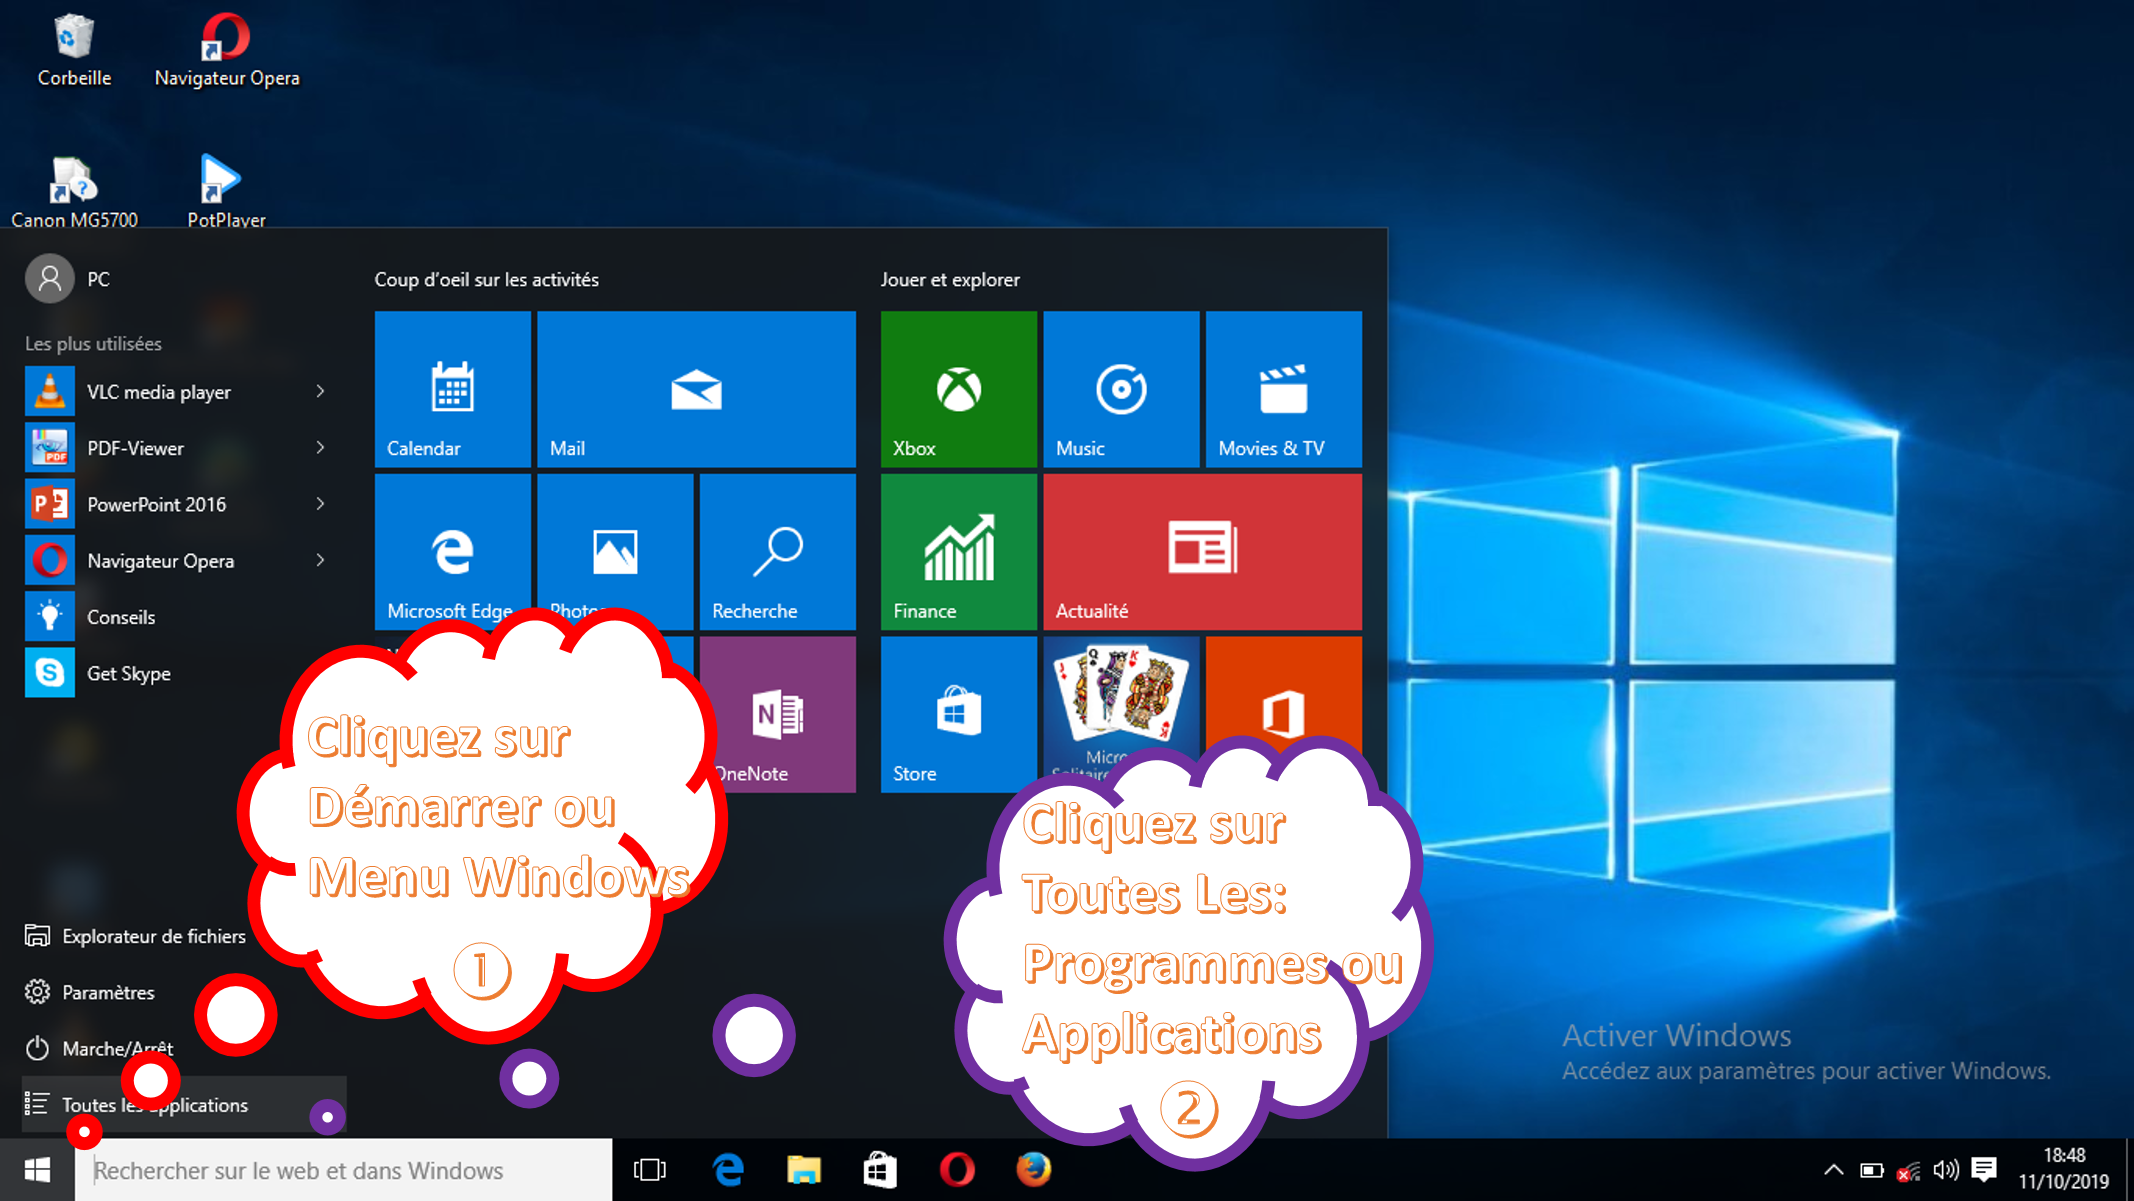
\includegraphics[ width=\linewidth,height=0.705\paperheight]{img/1}
	\end{landscape}
	\begin{landscape} 		
		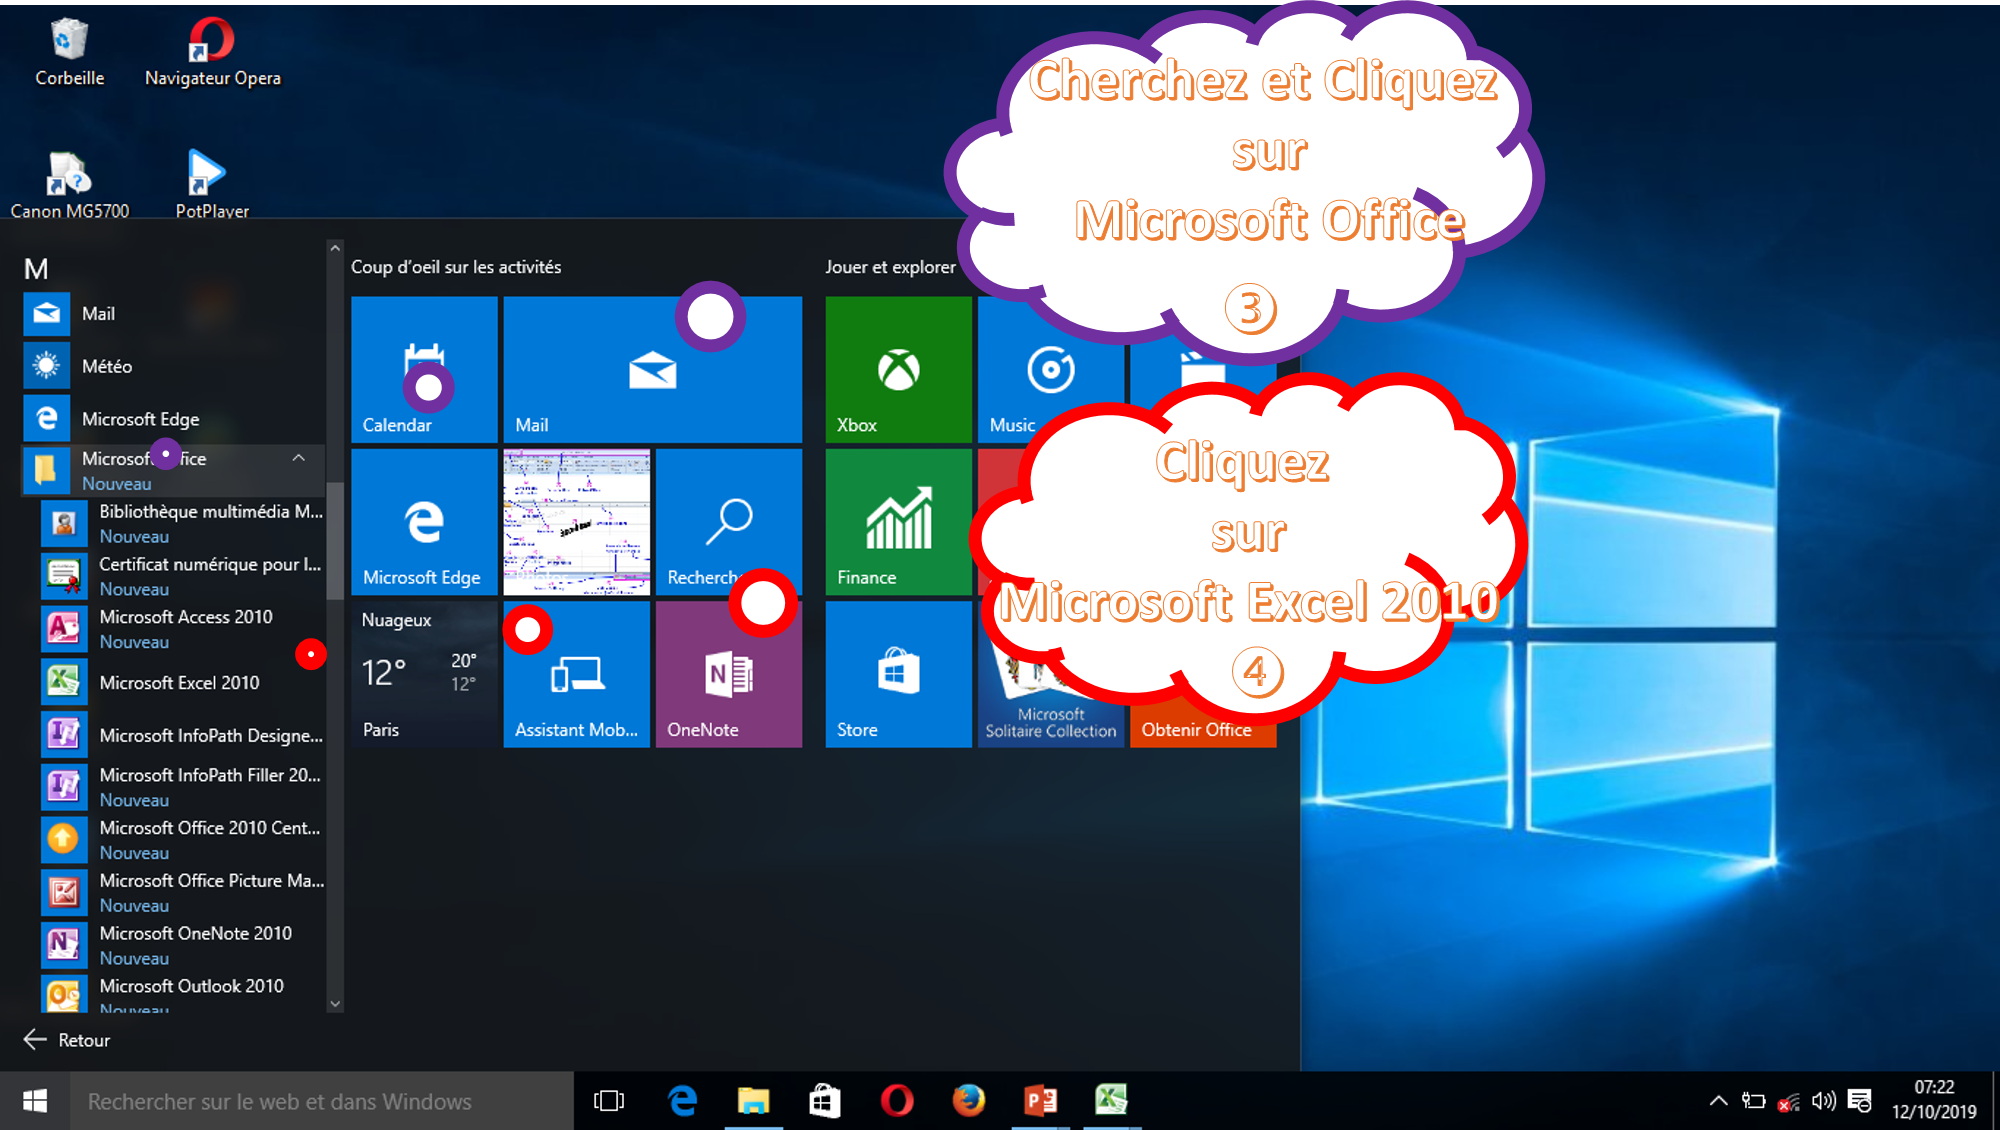
\includegraphics[ width=\linewidth,height=0.705\paperheight]{img/2}
	\end{landscape}
\begin{landscape} 		
	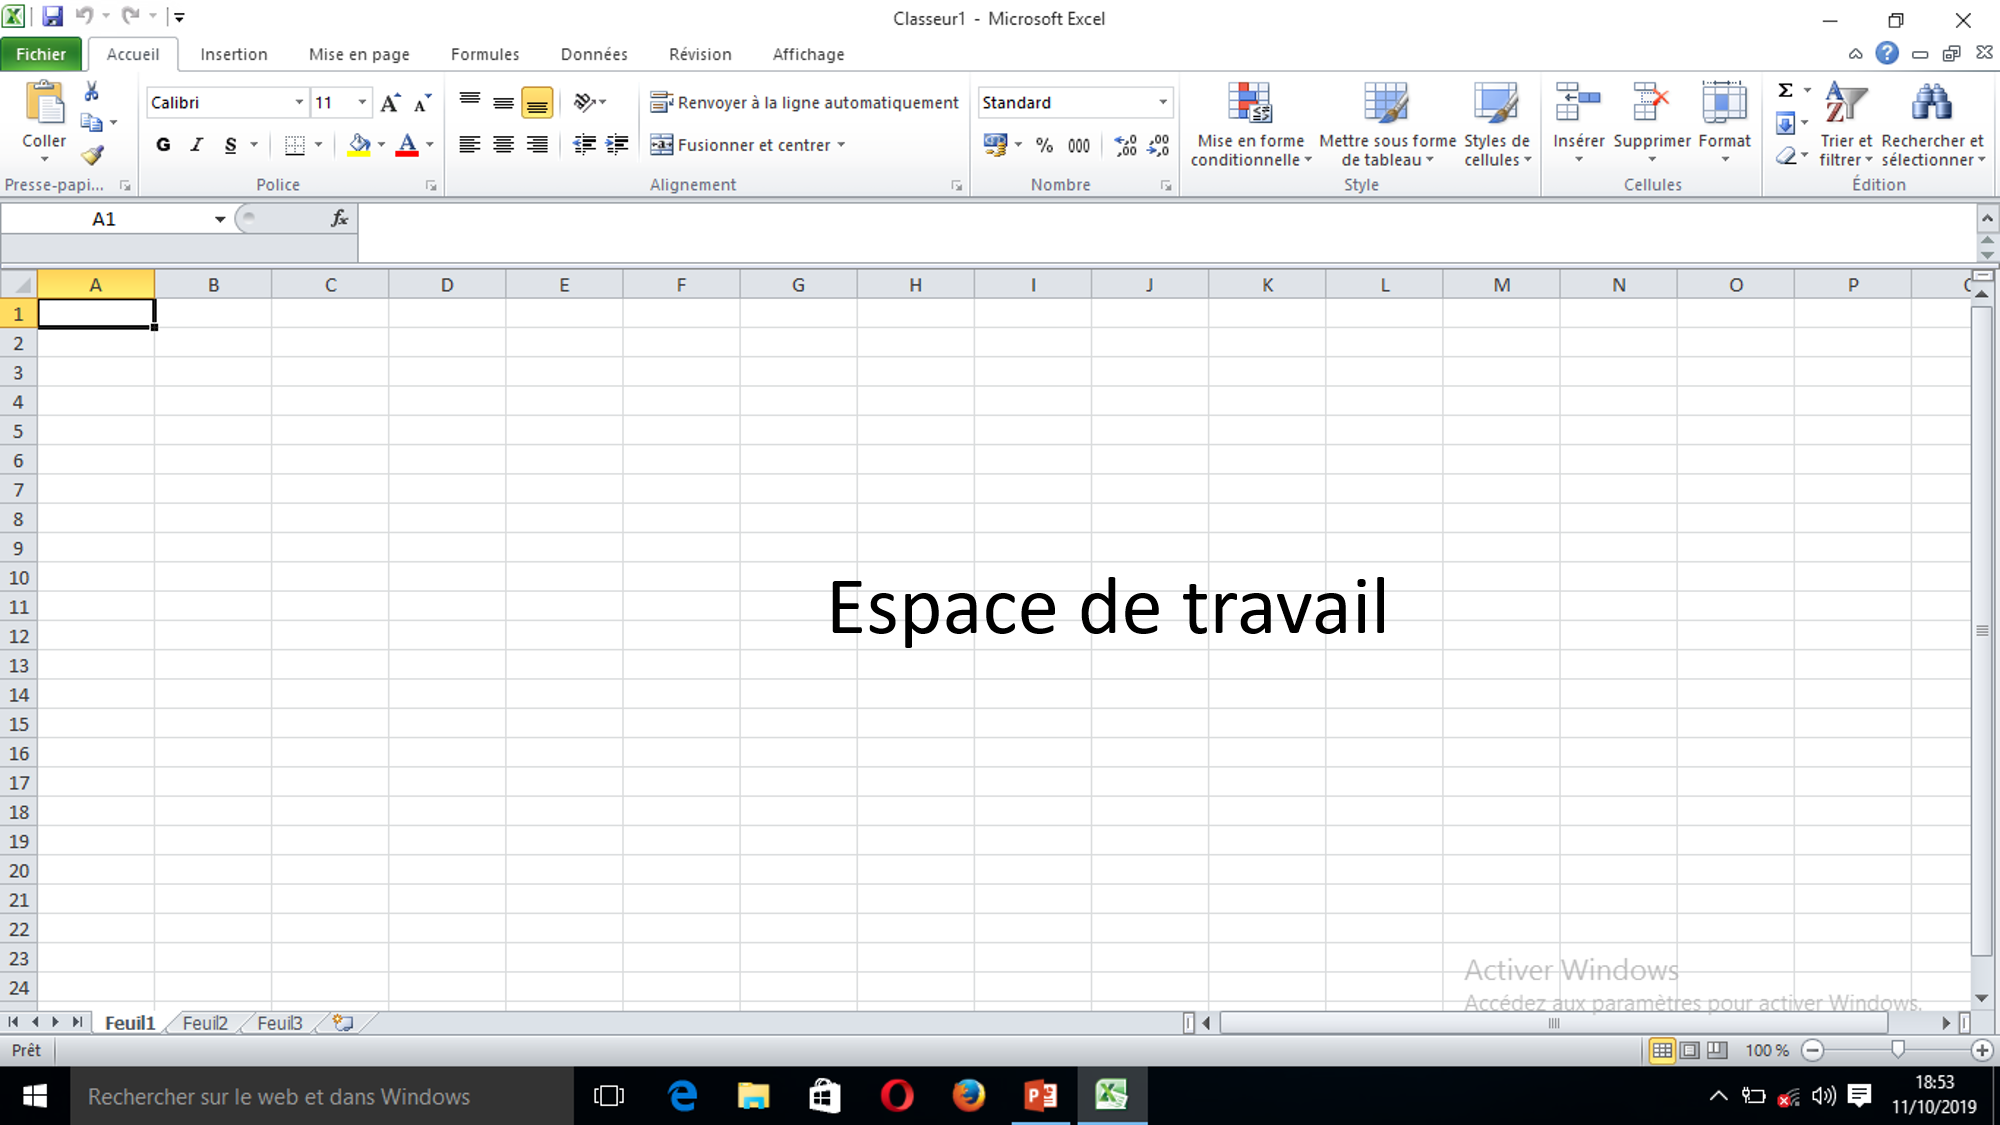
\includegraphics[ width=\linewidth,height=0.705\paperheight]{img/3}
\end{landscape}

\part{Presentation d'Excel}

\begin{landscape} 		
	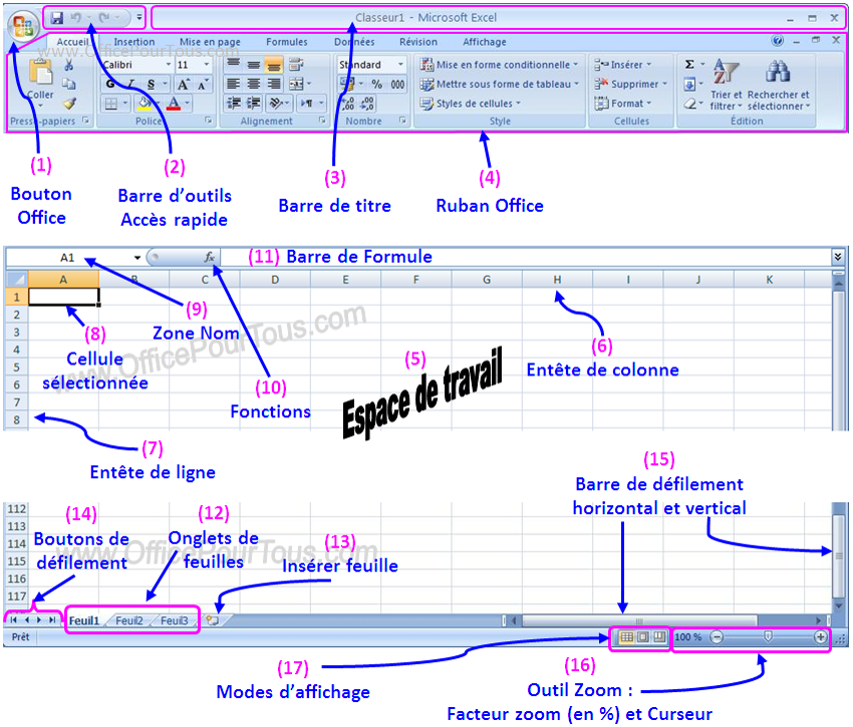
\includegraphics[ width=\linewidth,height=0.705\paperheight]{img/4}
\end{landscape}

\part{Creation d'un Nouveau Classeur}
\begin{landscape} 		
	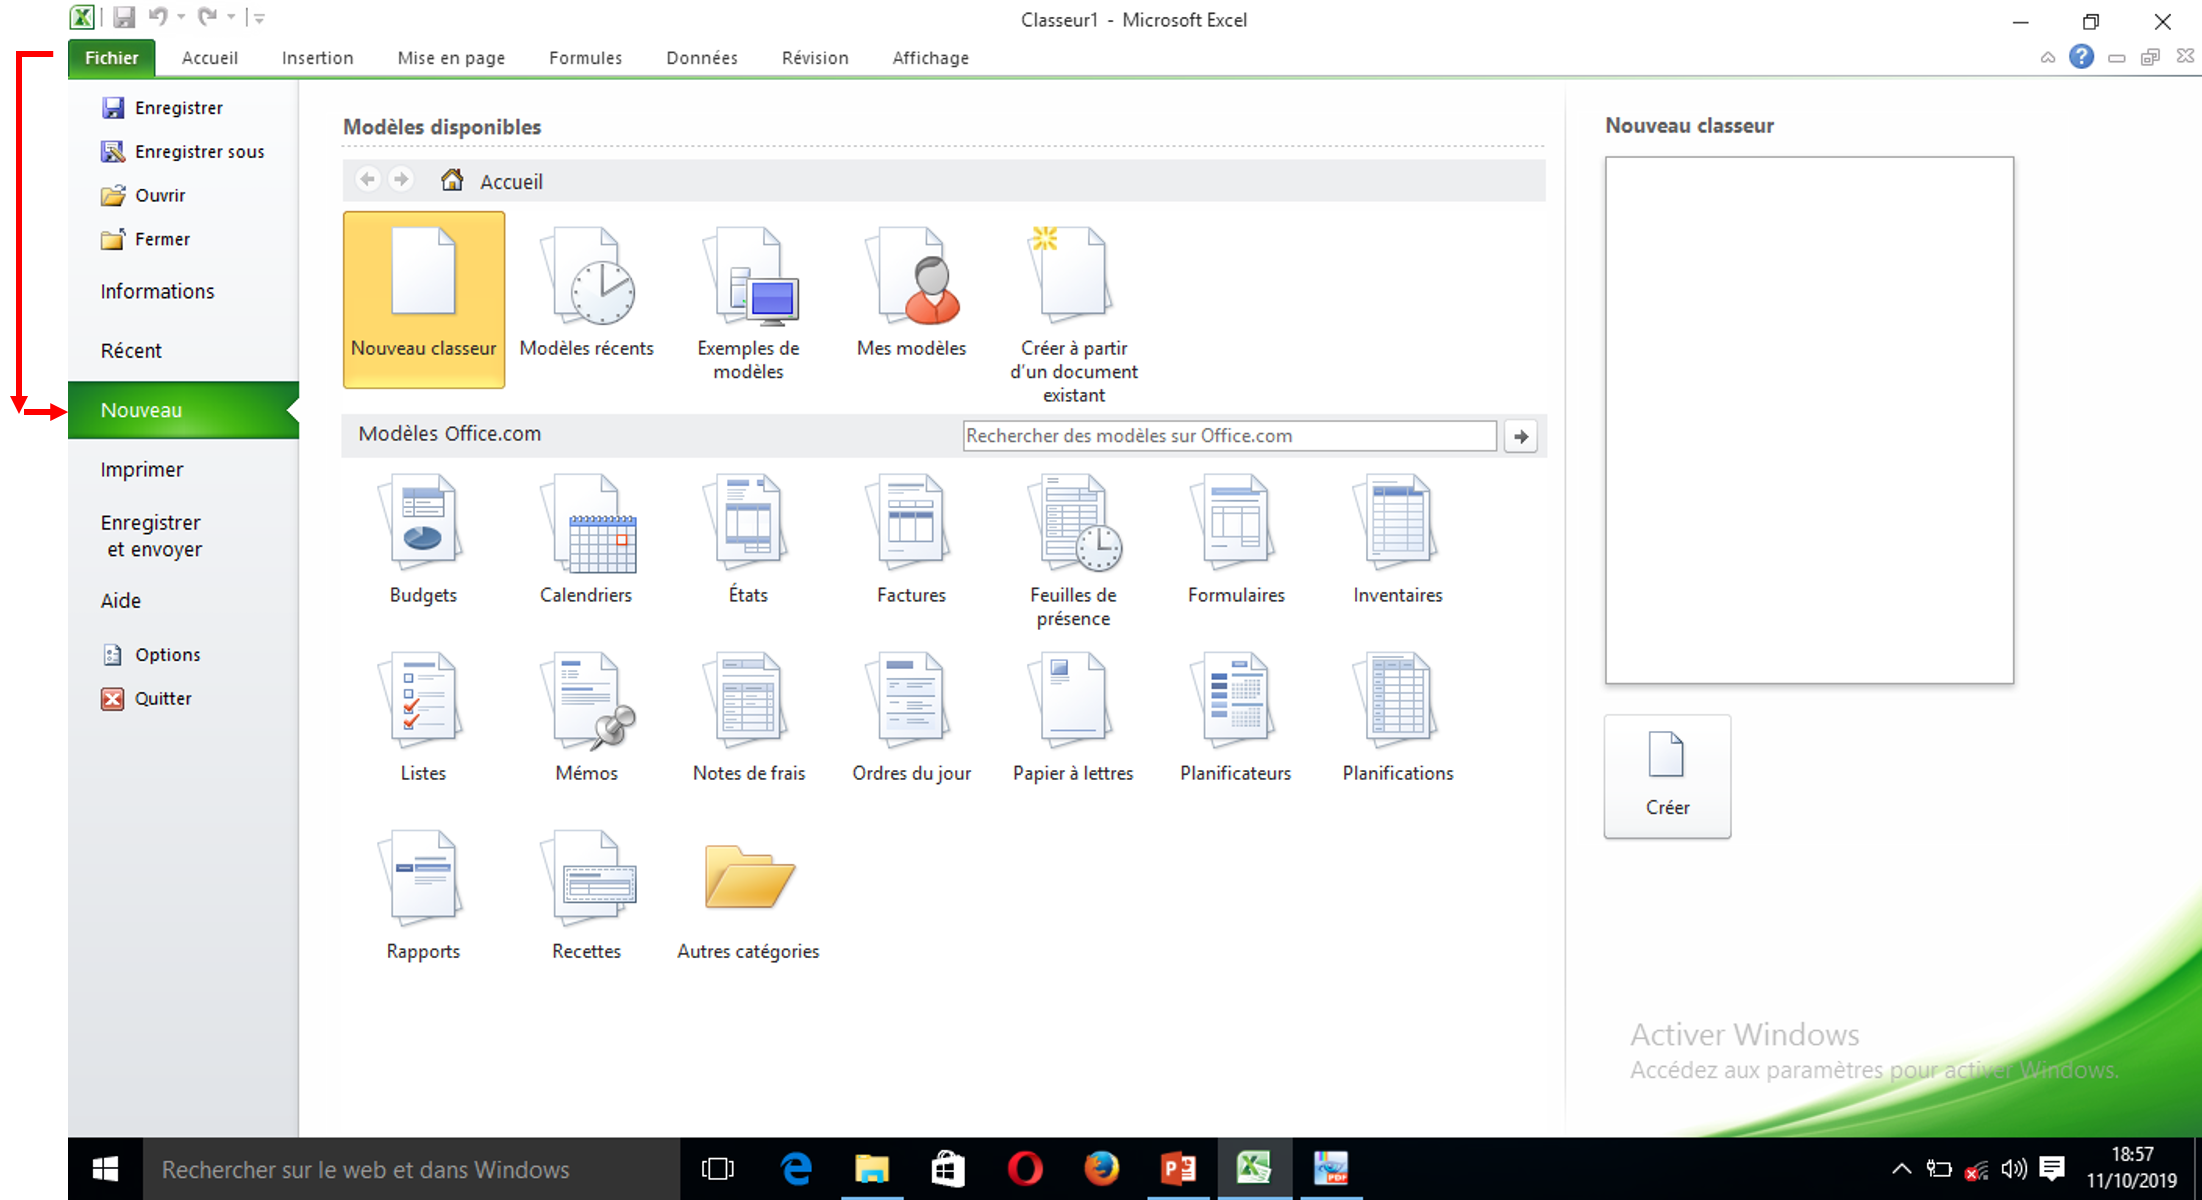
\includegraphics[ width=\linewidth,height=0.705\paperheight]{img/5}
\end{landscape}
\begin{landscape} 		
	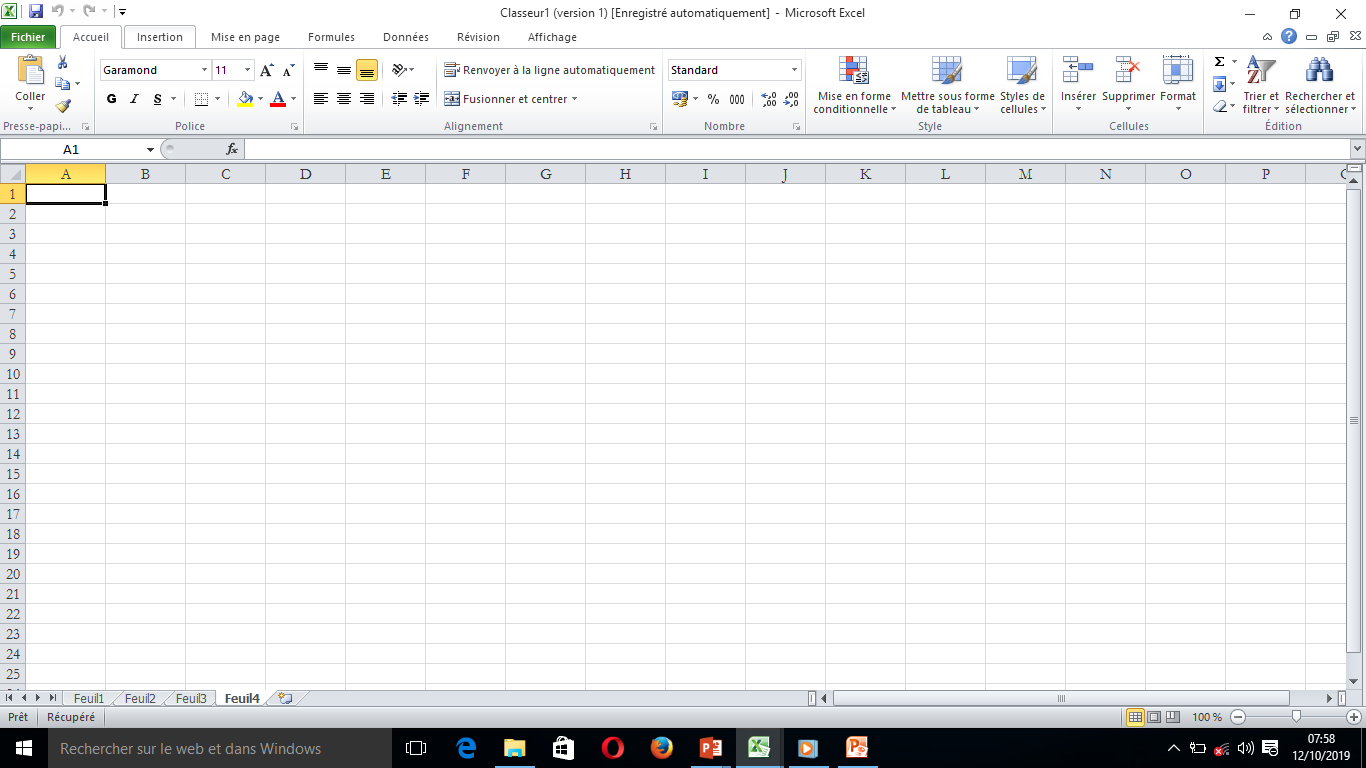
\includegraphics[ width=\linewidth,height=0.705\paperheight]{img/6}
\end{landscape}

\part{Enregistrer la premiere fois}
\begin{landscape} 		
	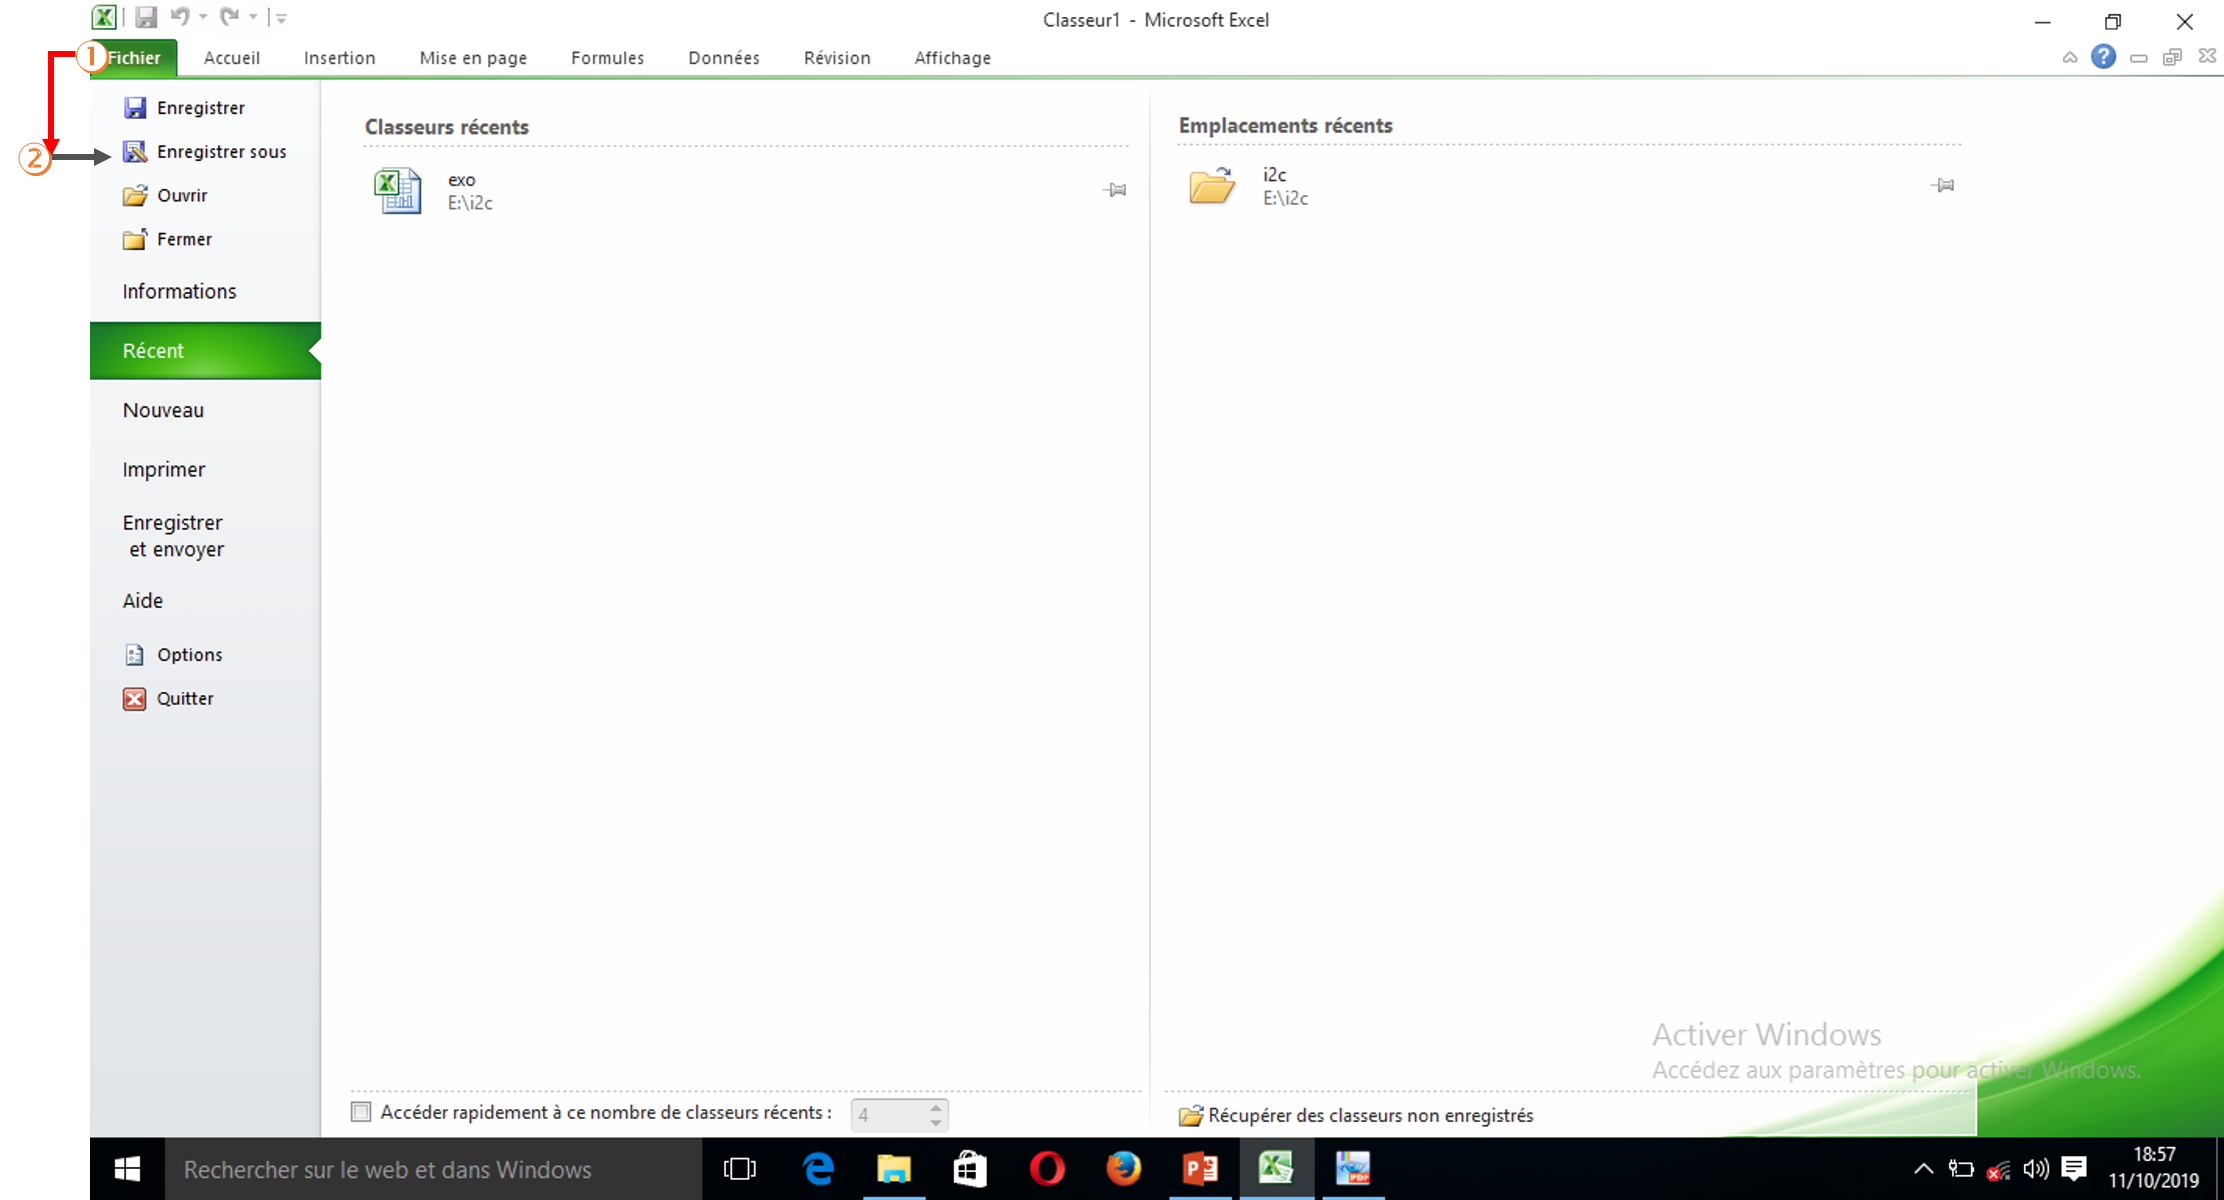
\includegraphics[ width=\linewidth,height=0.705\paperheight]{img/7}
\end{landscape}

\part{Enregistrer \& Fermer}


\begin{landscape} 		
	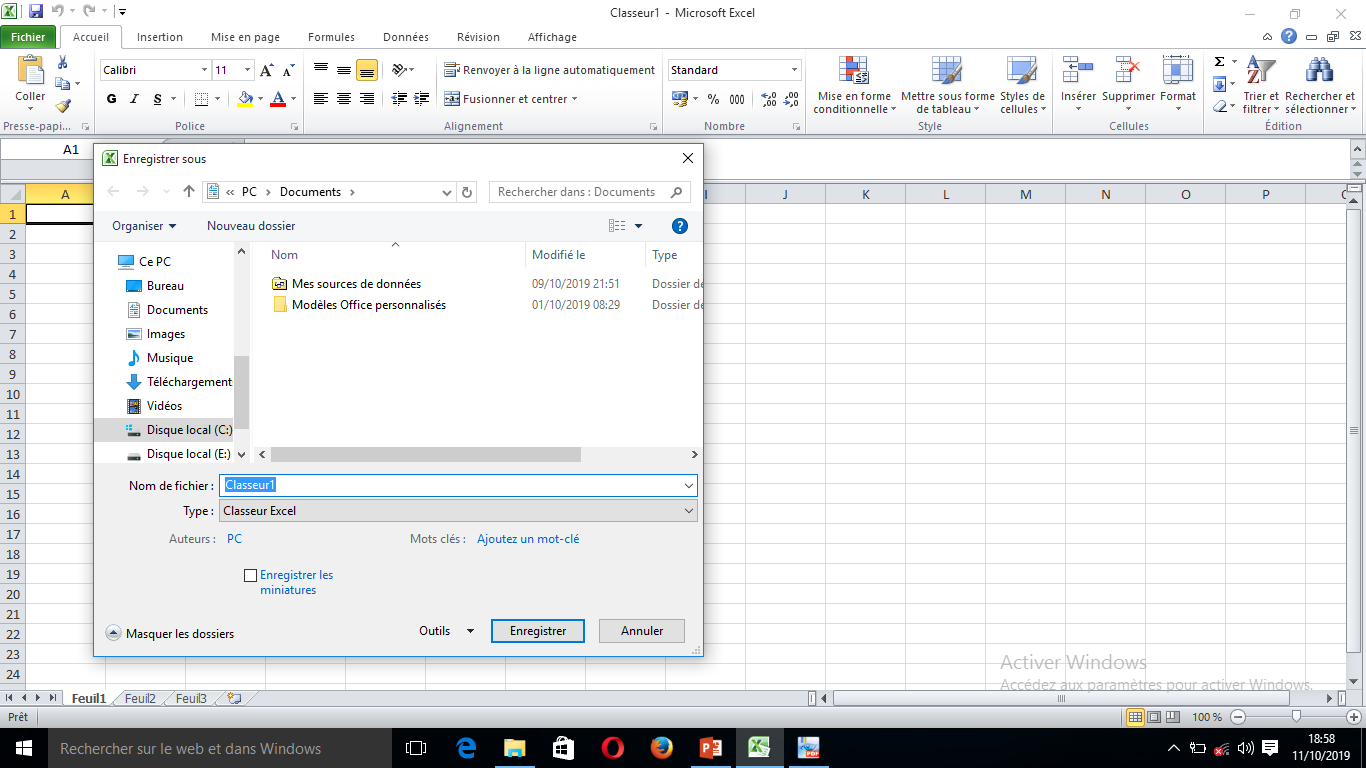
\includegraphics[ width=\linewidth,height=0.705\paperheight]{img/8}
\end{landscape}

\part{Insertion d'image}
\begin{landscape} 		
	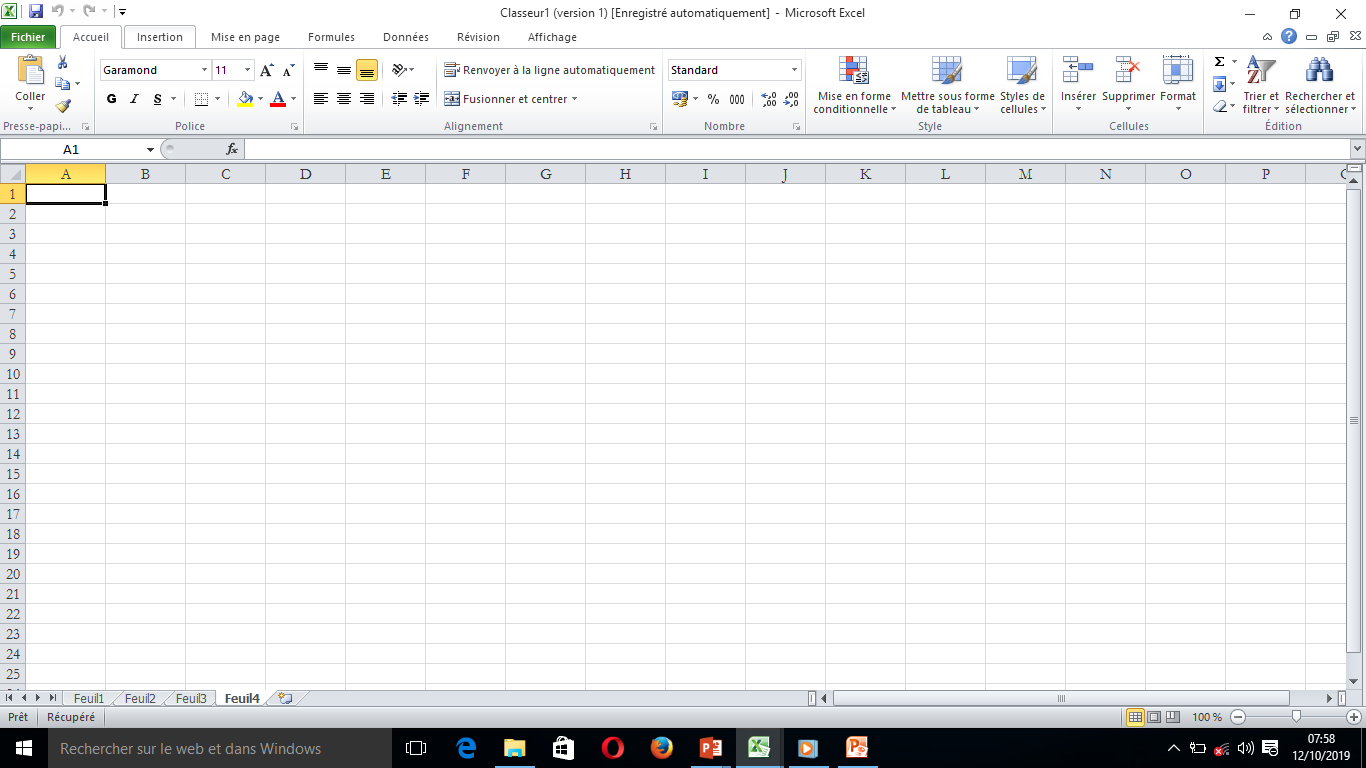
\includegraphics[ width=\linewidth,height=0.705\paperheight]{img/9}
\end{landscape}
\begin{landscape} 		
	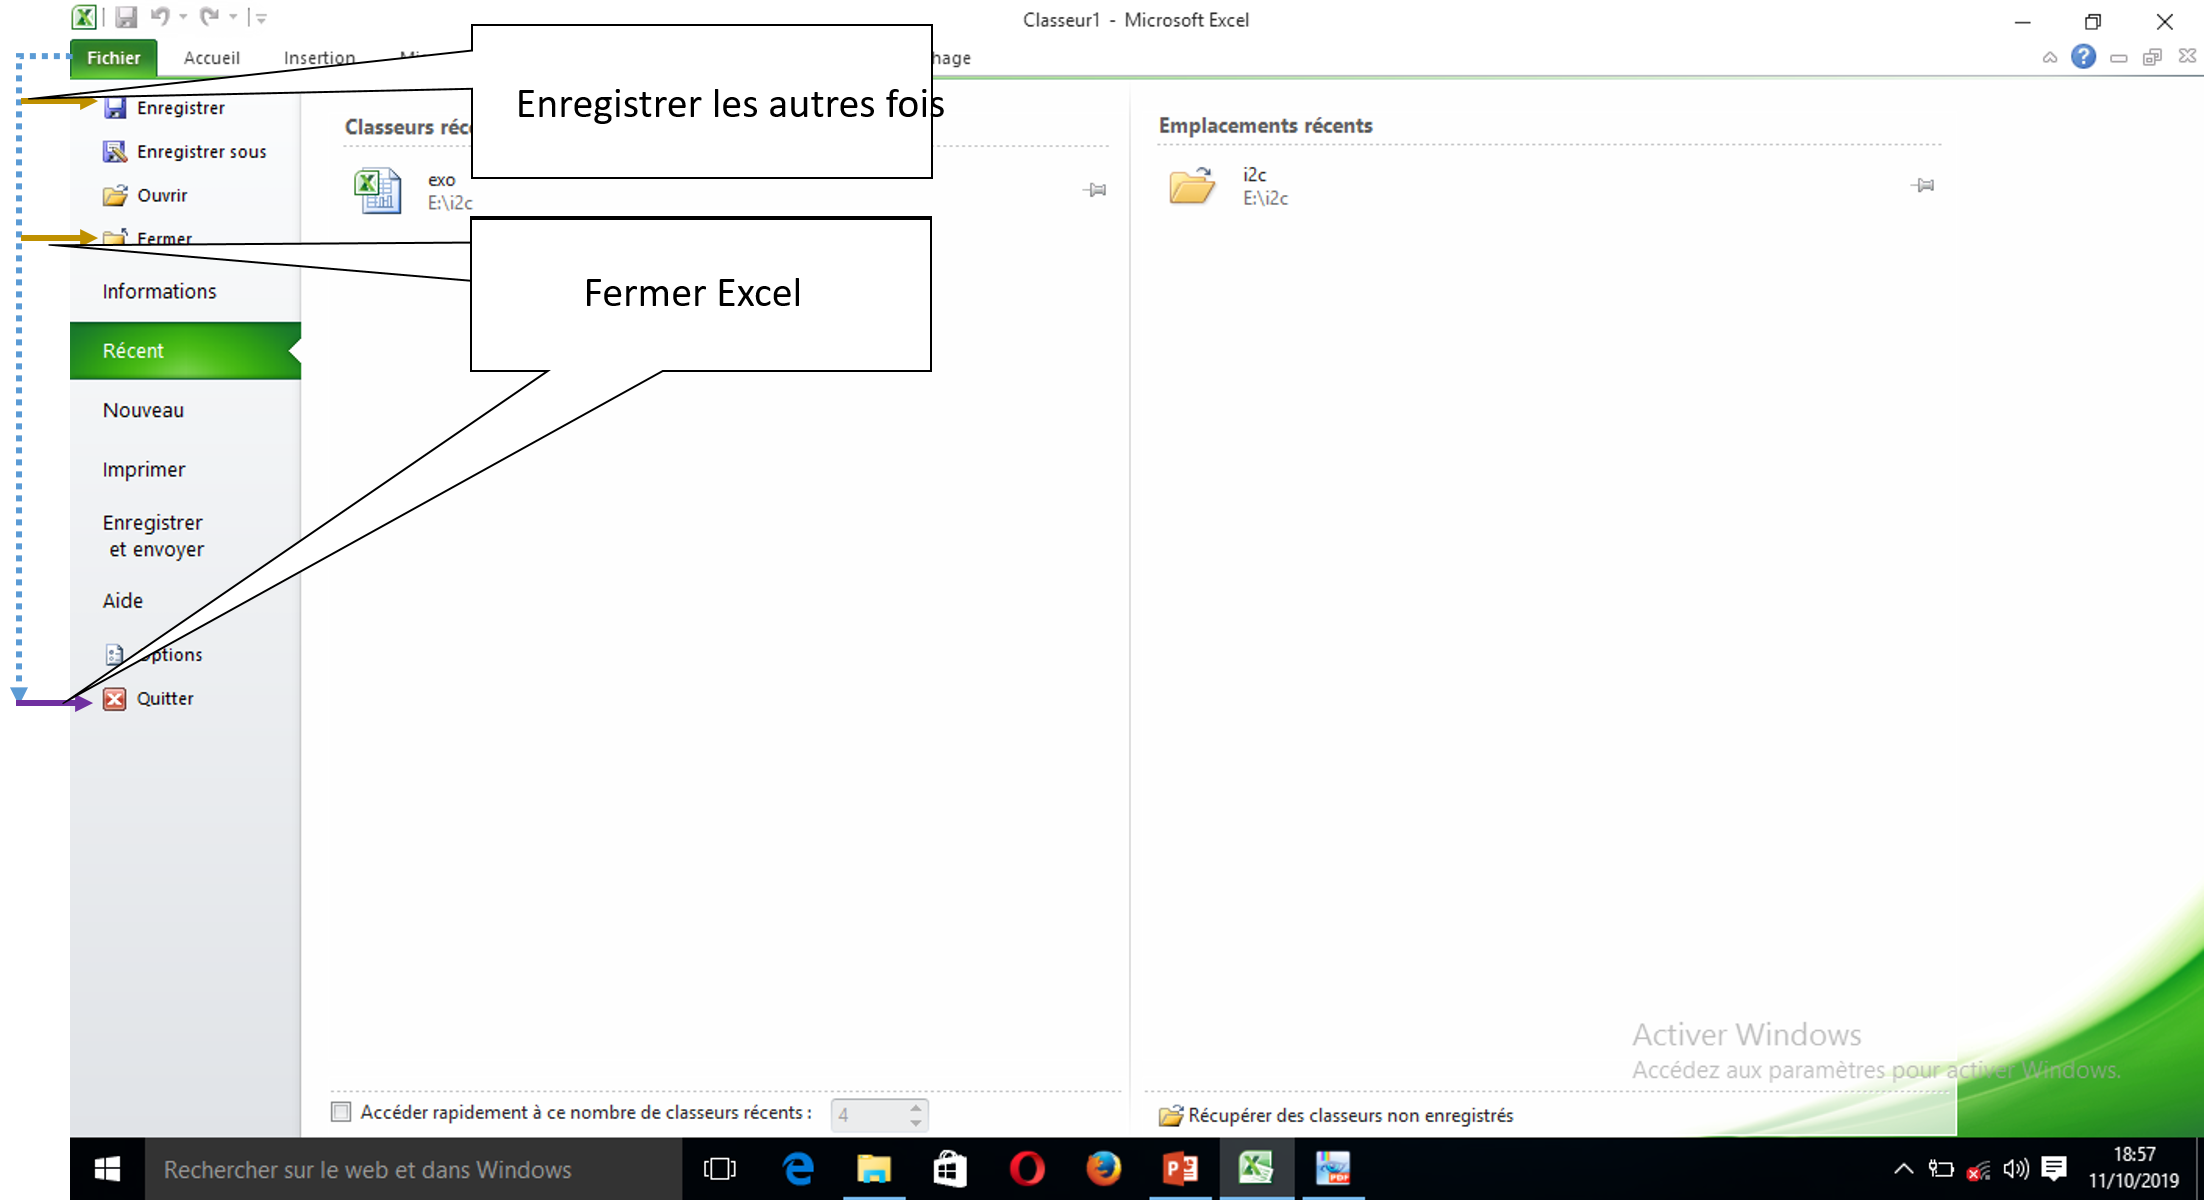
\includegraphics[ width=\linewidth,height=0.705\paperheight]{img/10}
\end{landscape}
\begin{landscape} 		
	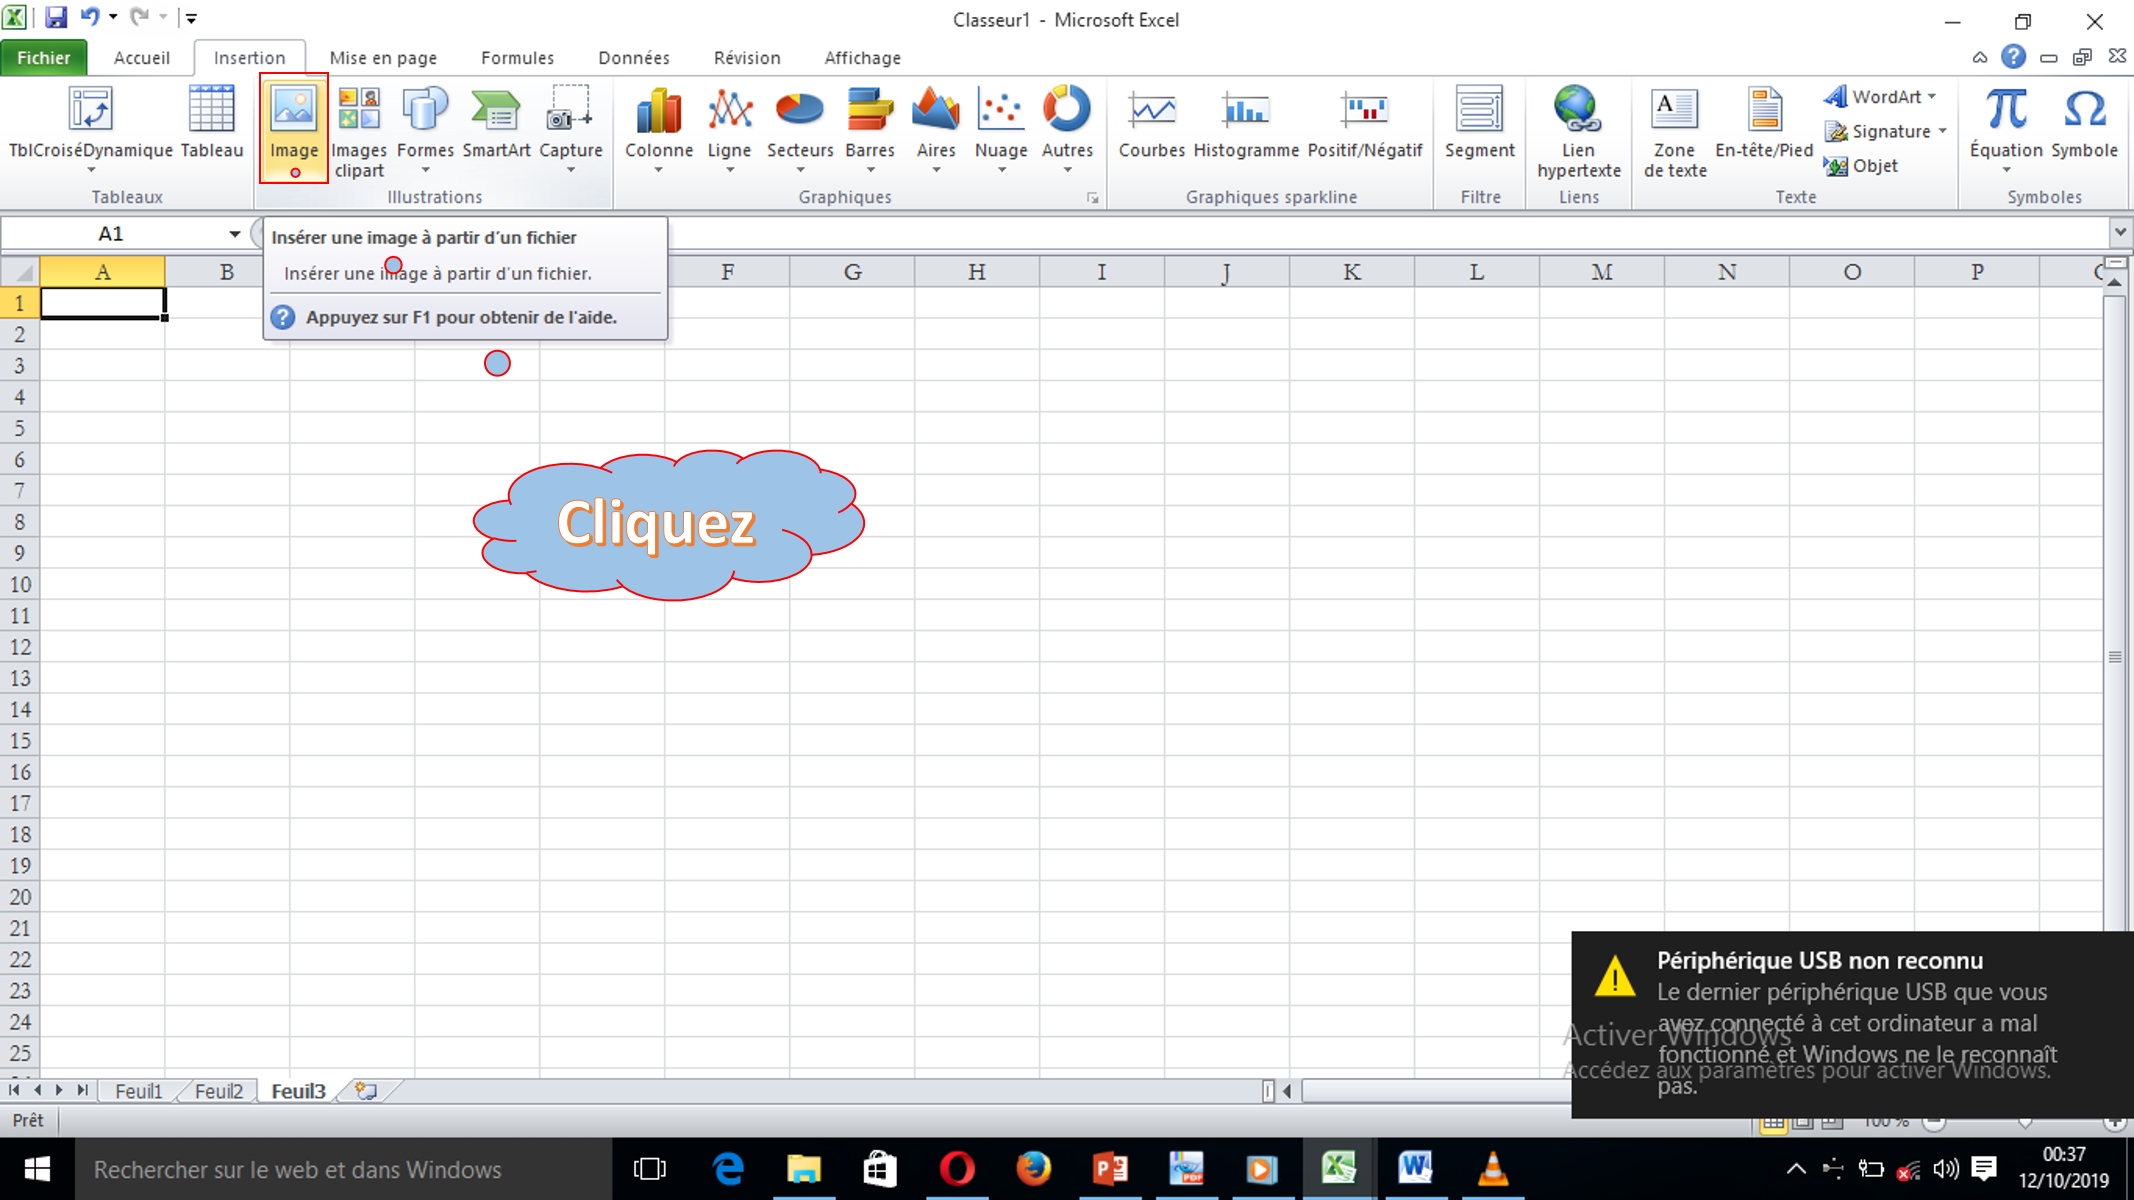
\includegraphics[ width=\linewidth,height=0.705\paperheight]{img/11}
\end{landscape}
\begin{landscape} 		
	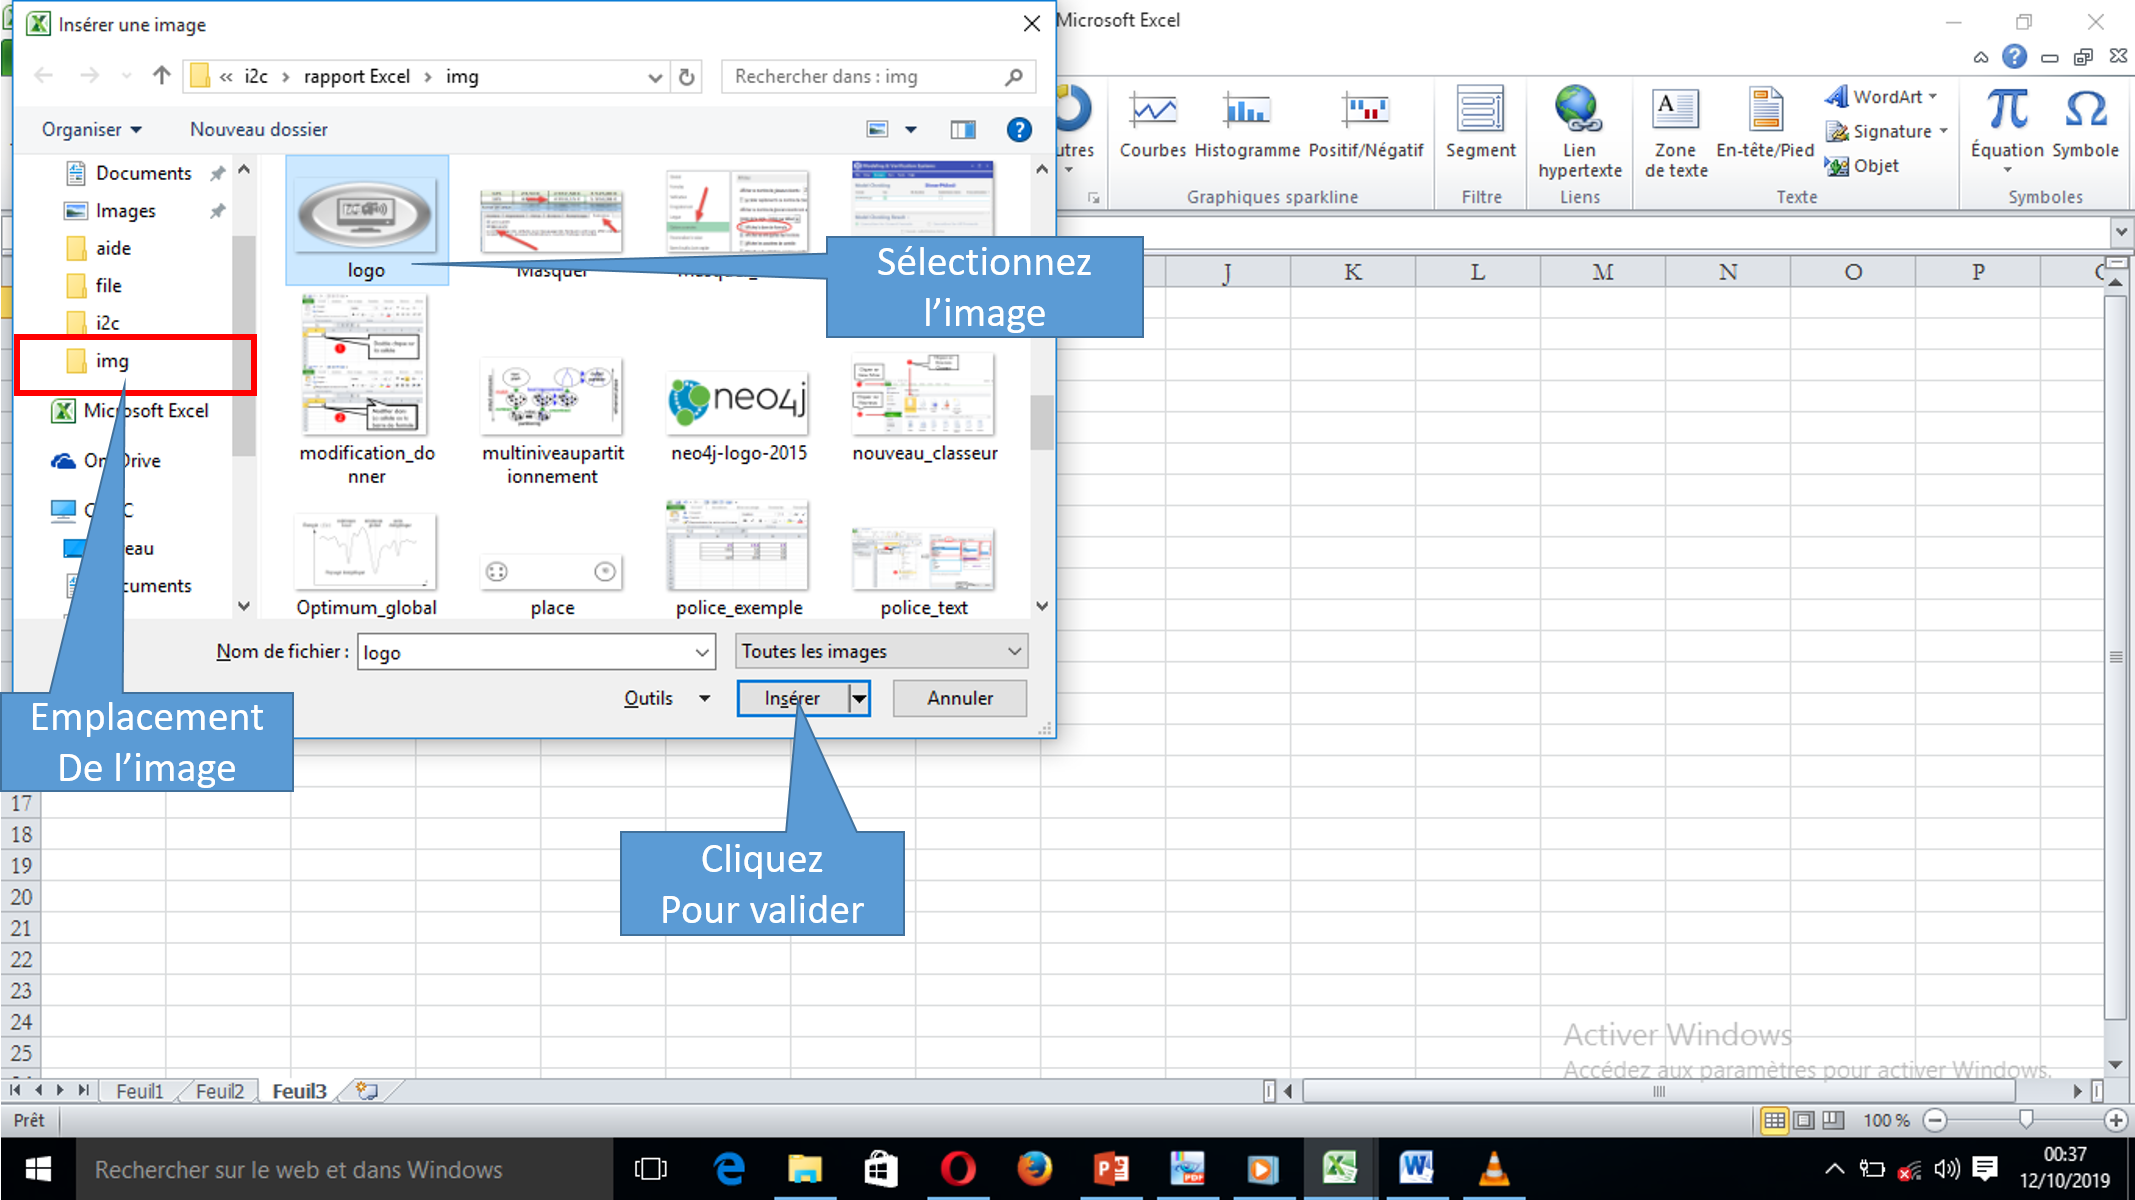
\includegraphics[ width=\linewidth,height=0.705\paperheight]{img/12}
\end{landscape}

\part{Saisie Brute}
\begin{landscape} 		
	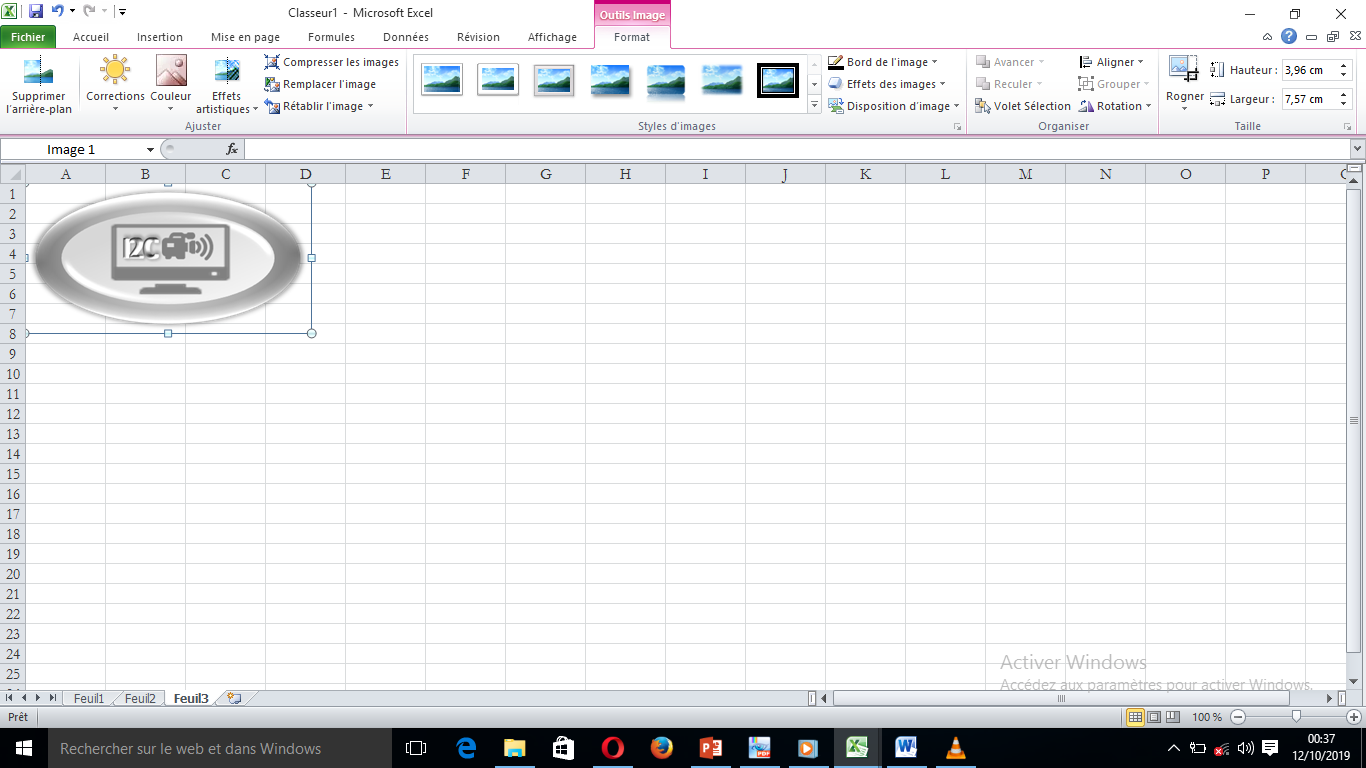
\includegraphics[ width=\linewidth,height=0.705\paperheight]{img/13}
\end{landscape}
\part{Mise en Forme}
\begin{landscape} 		
	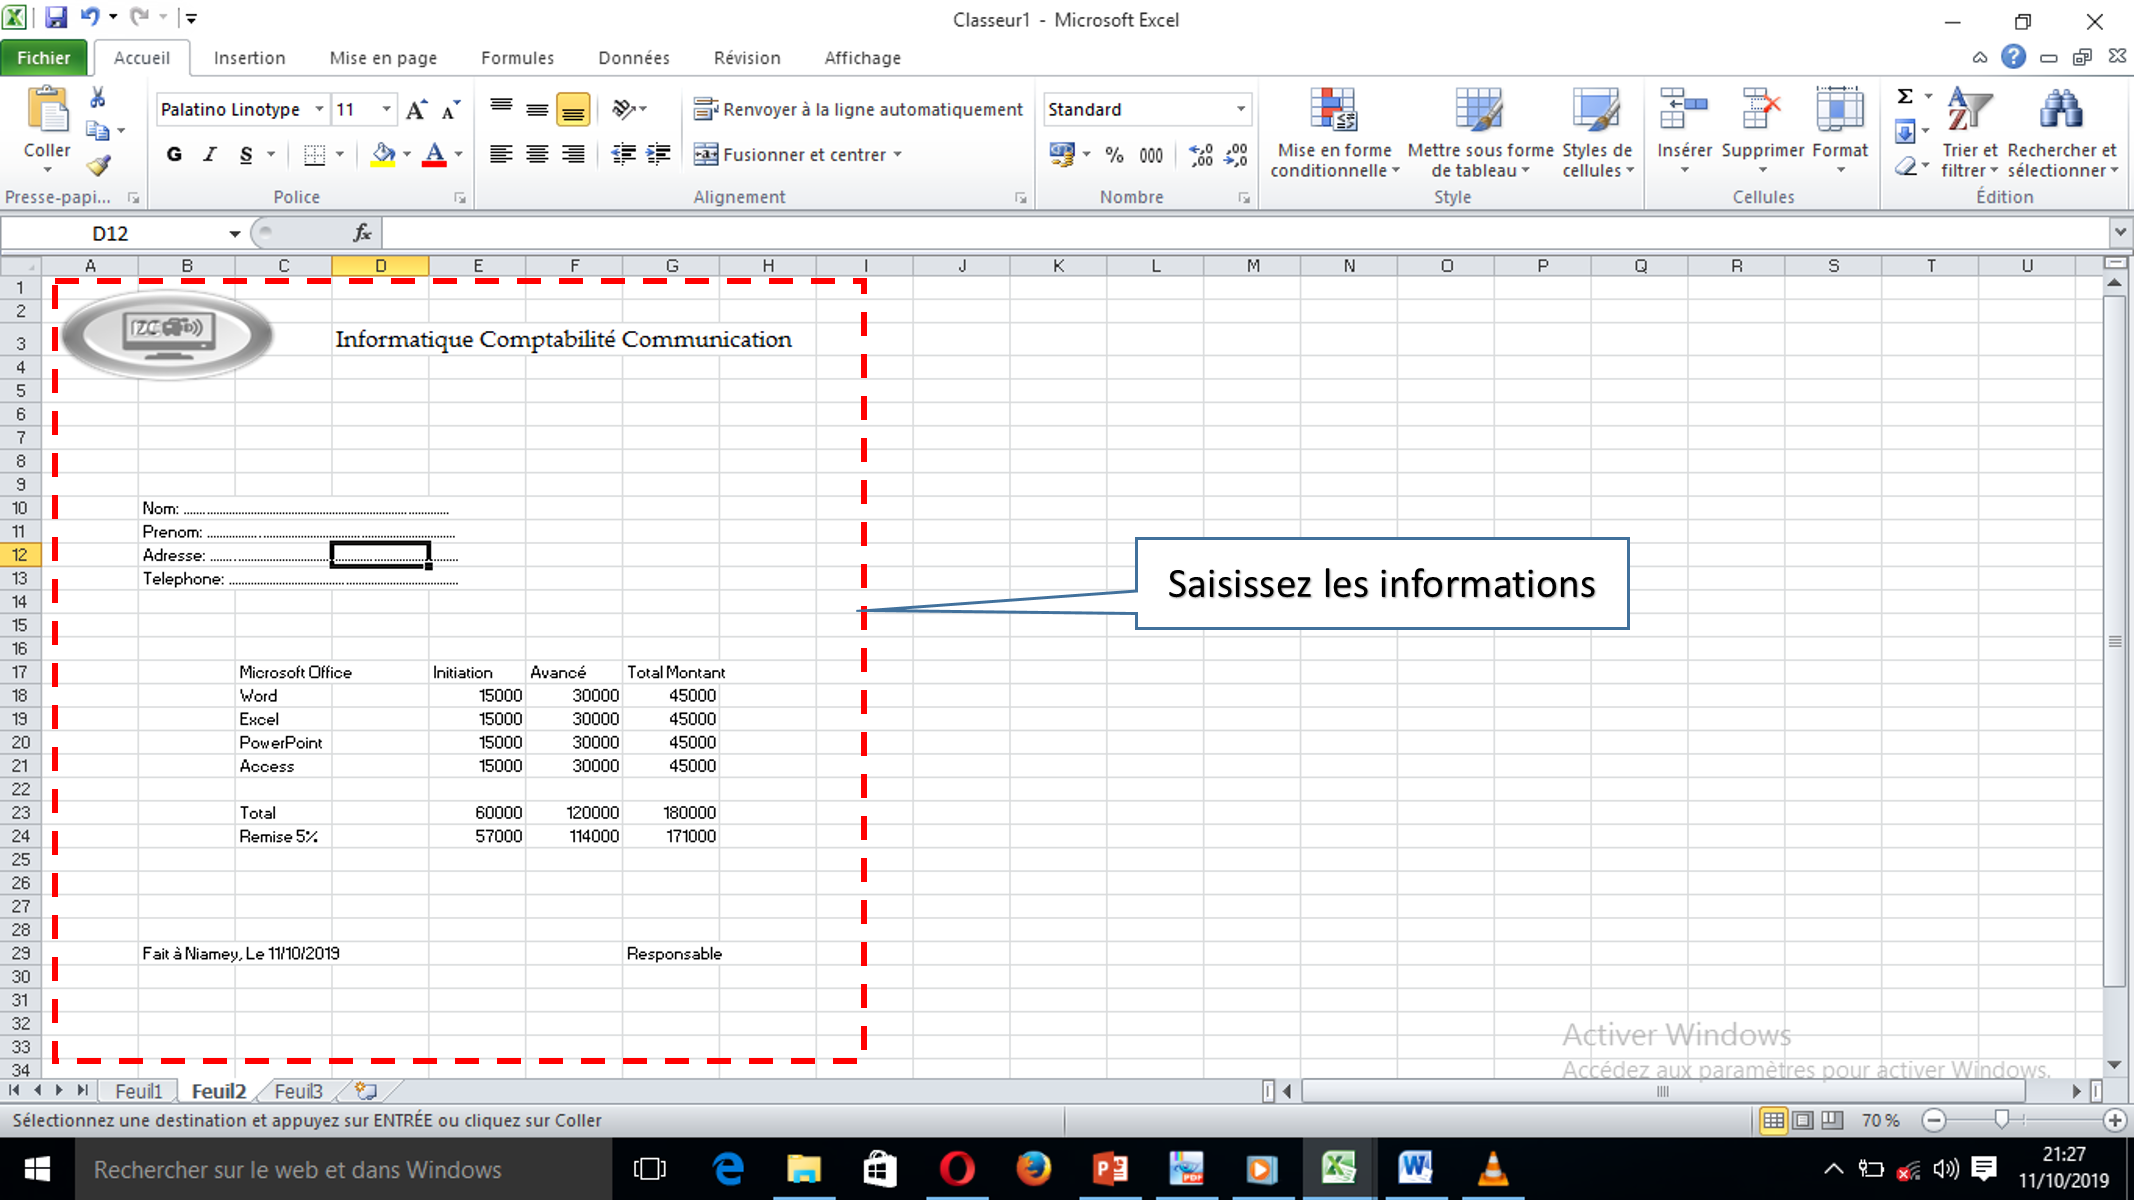
\includegraphics[ width=\linewidth,height=0.705\paperheight]{img/14}
\end{landscape}
\begin{landscape} 		
	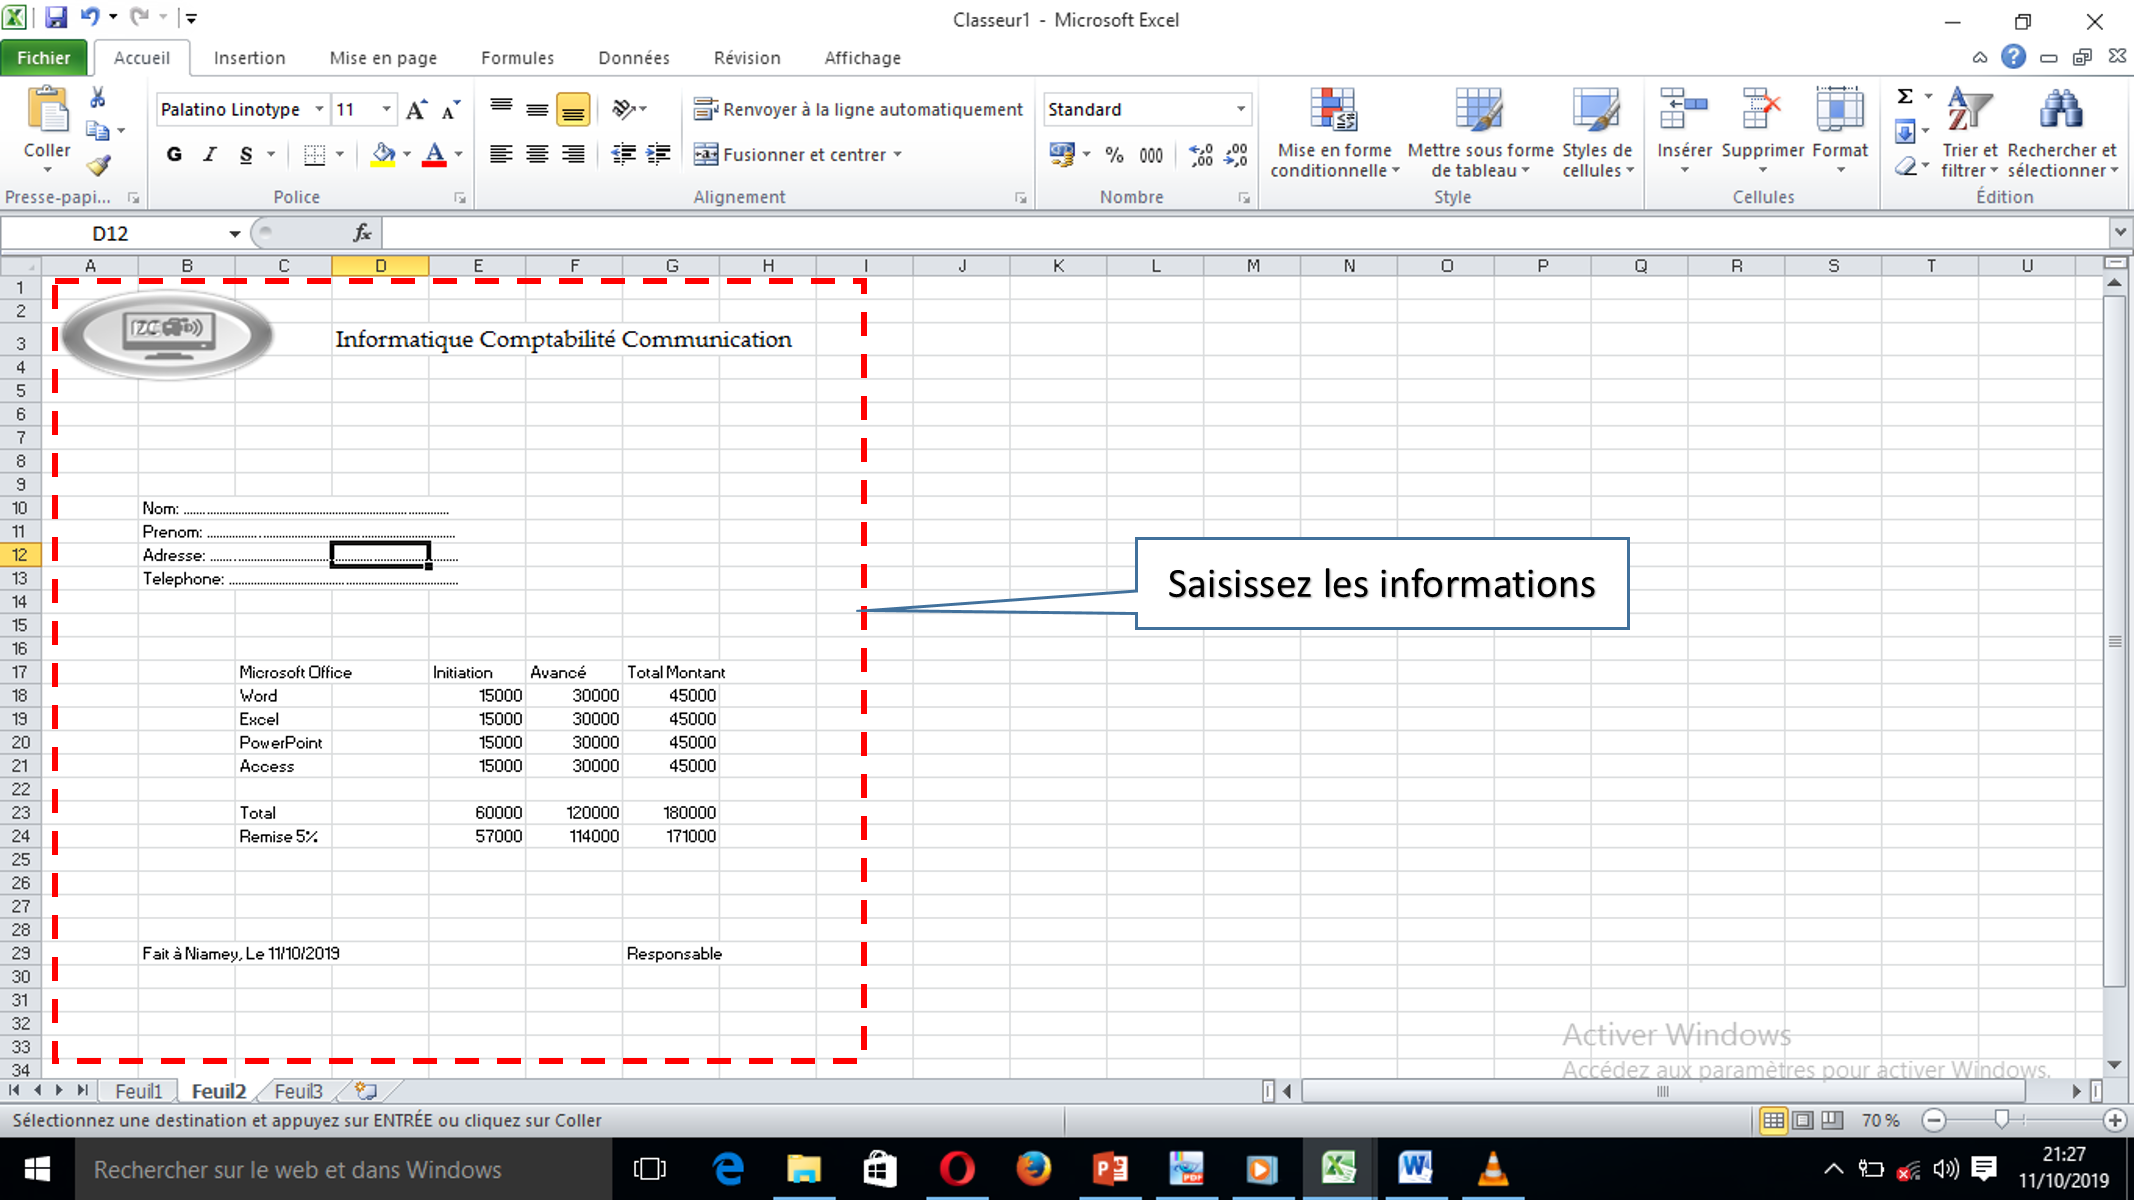
\includegraphics[ width=\linewidth,height=0.705\paperheight]{img/15}
\end{landscape}
\begin{landscape} 		
	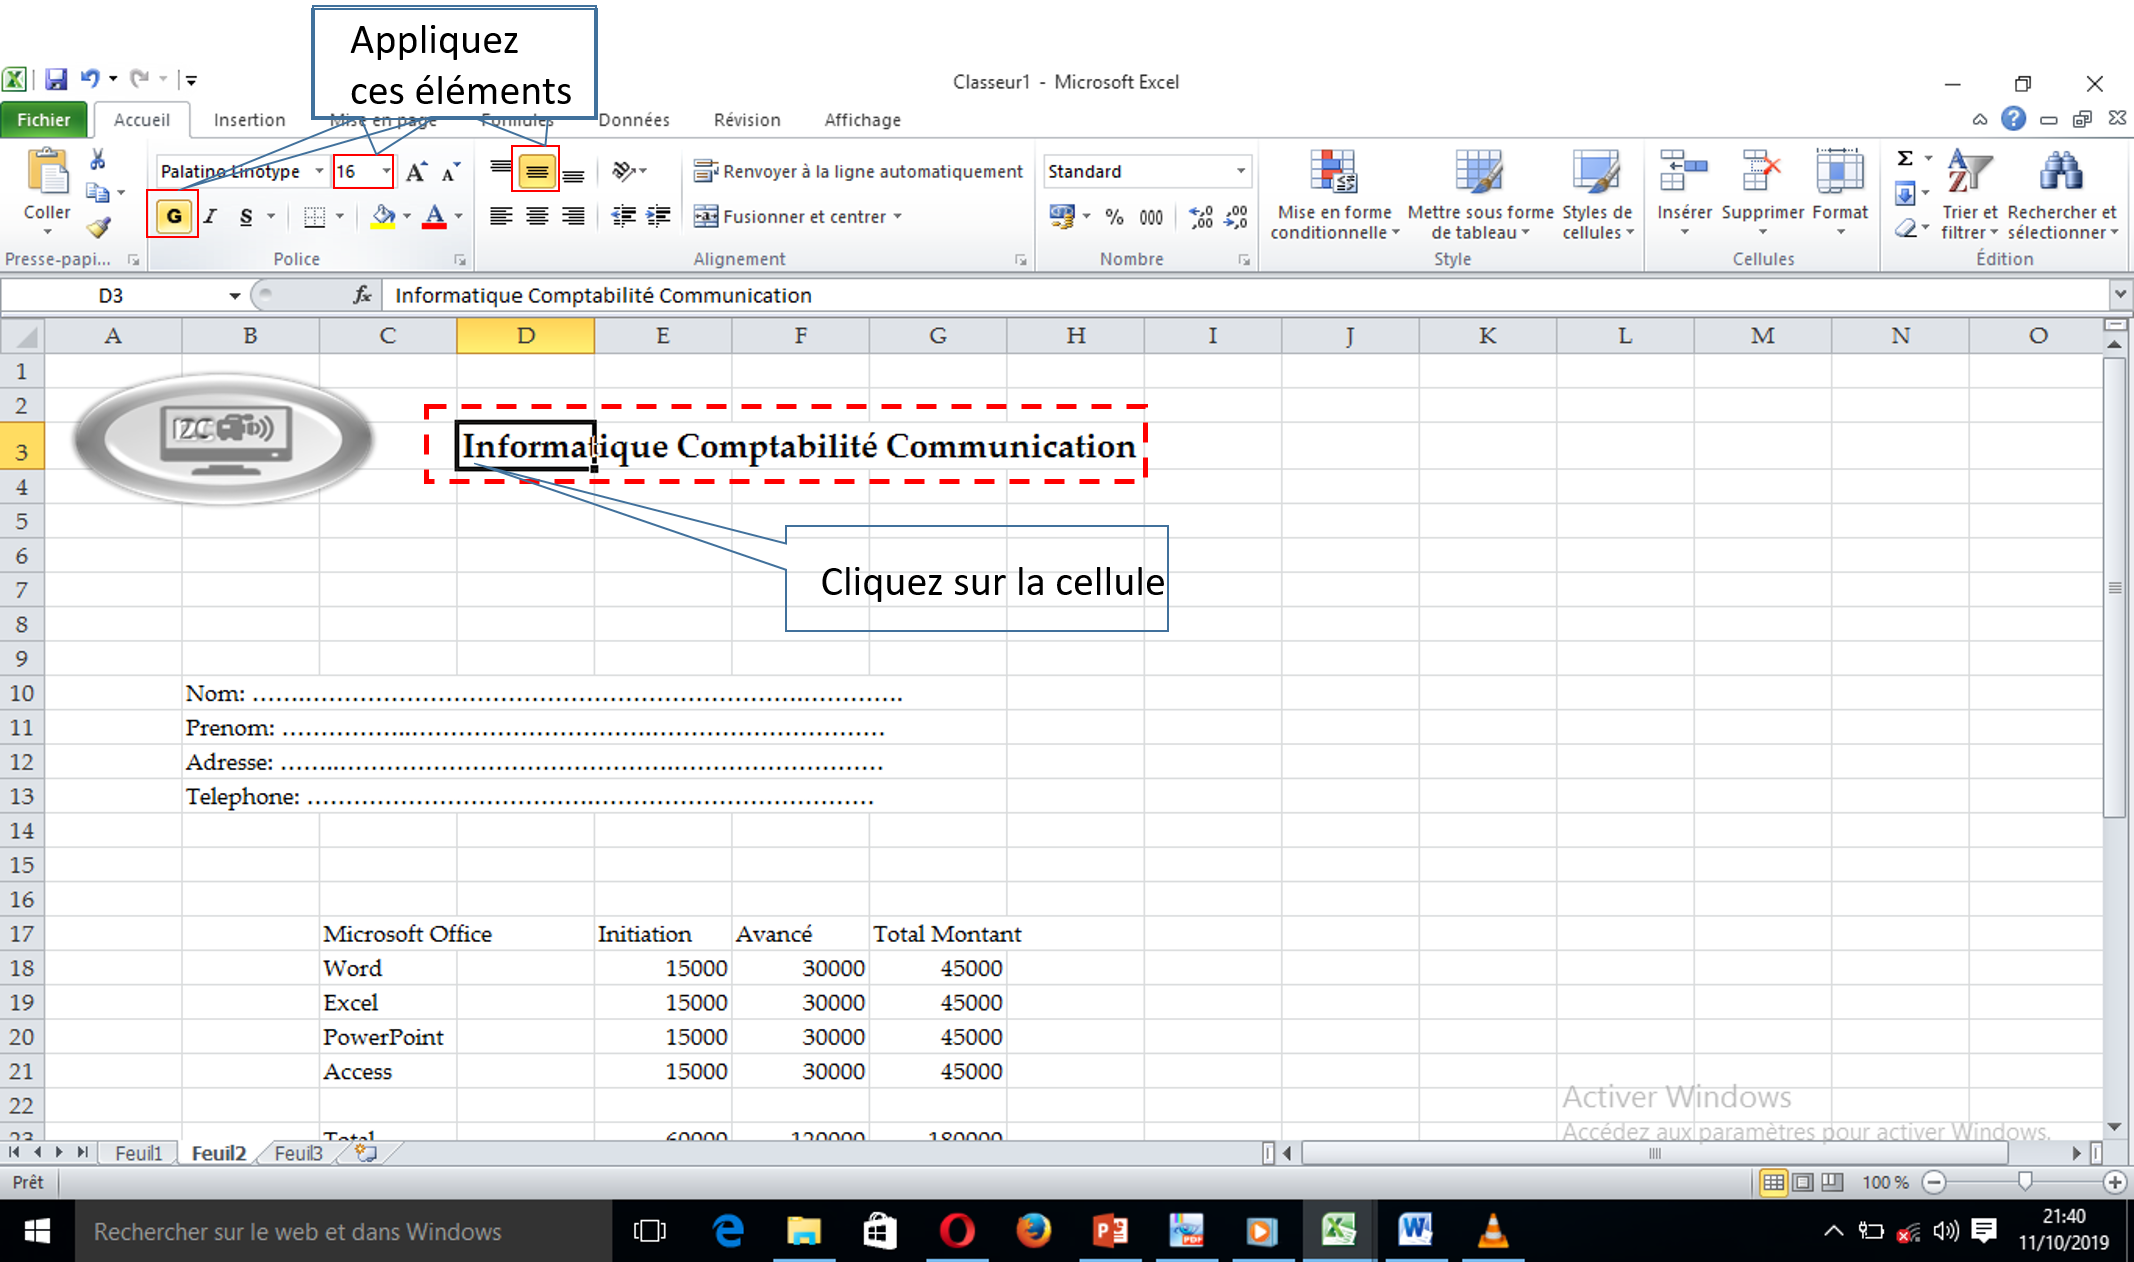
\includegraphics[ width=\linewidth,height=0.705\paperheight]{img/16}
\end{landscape}
\begin{landscape} 		
	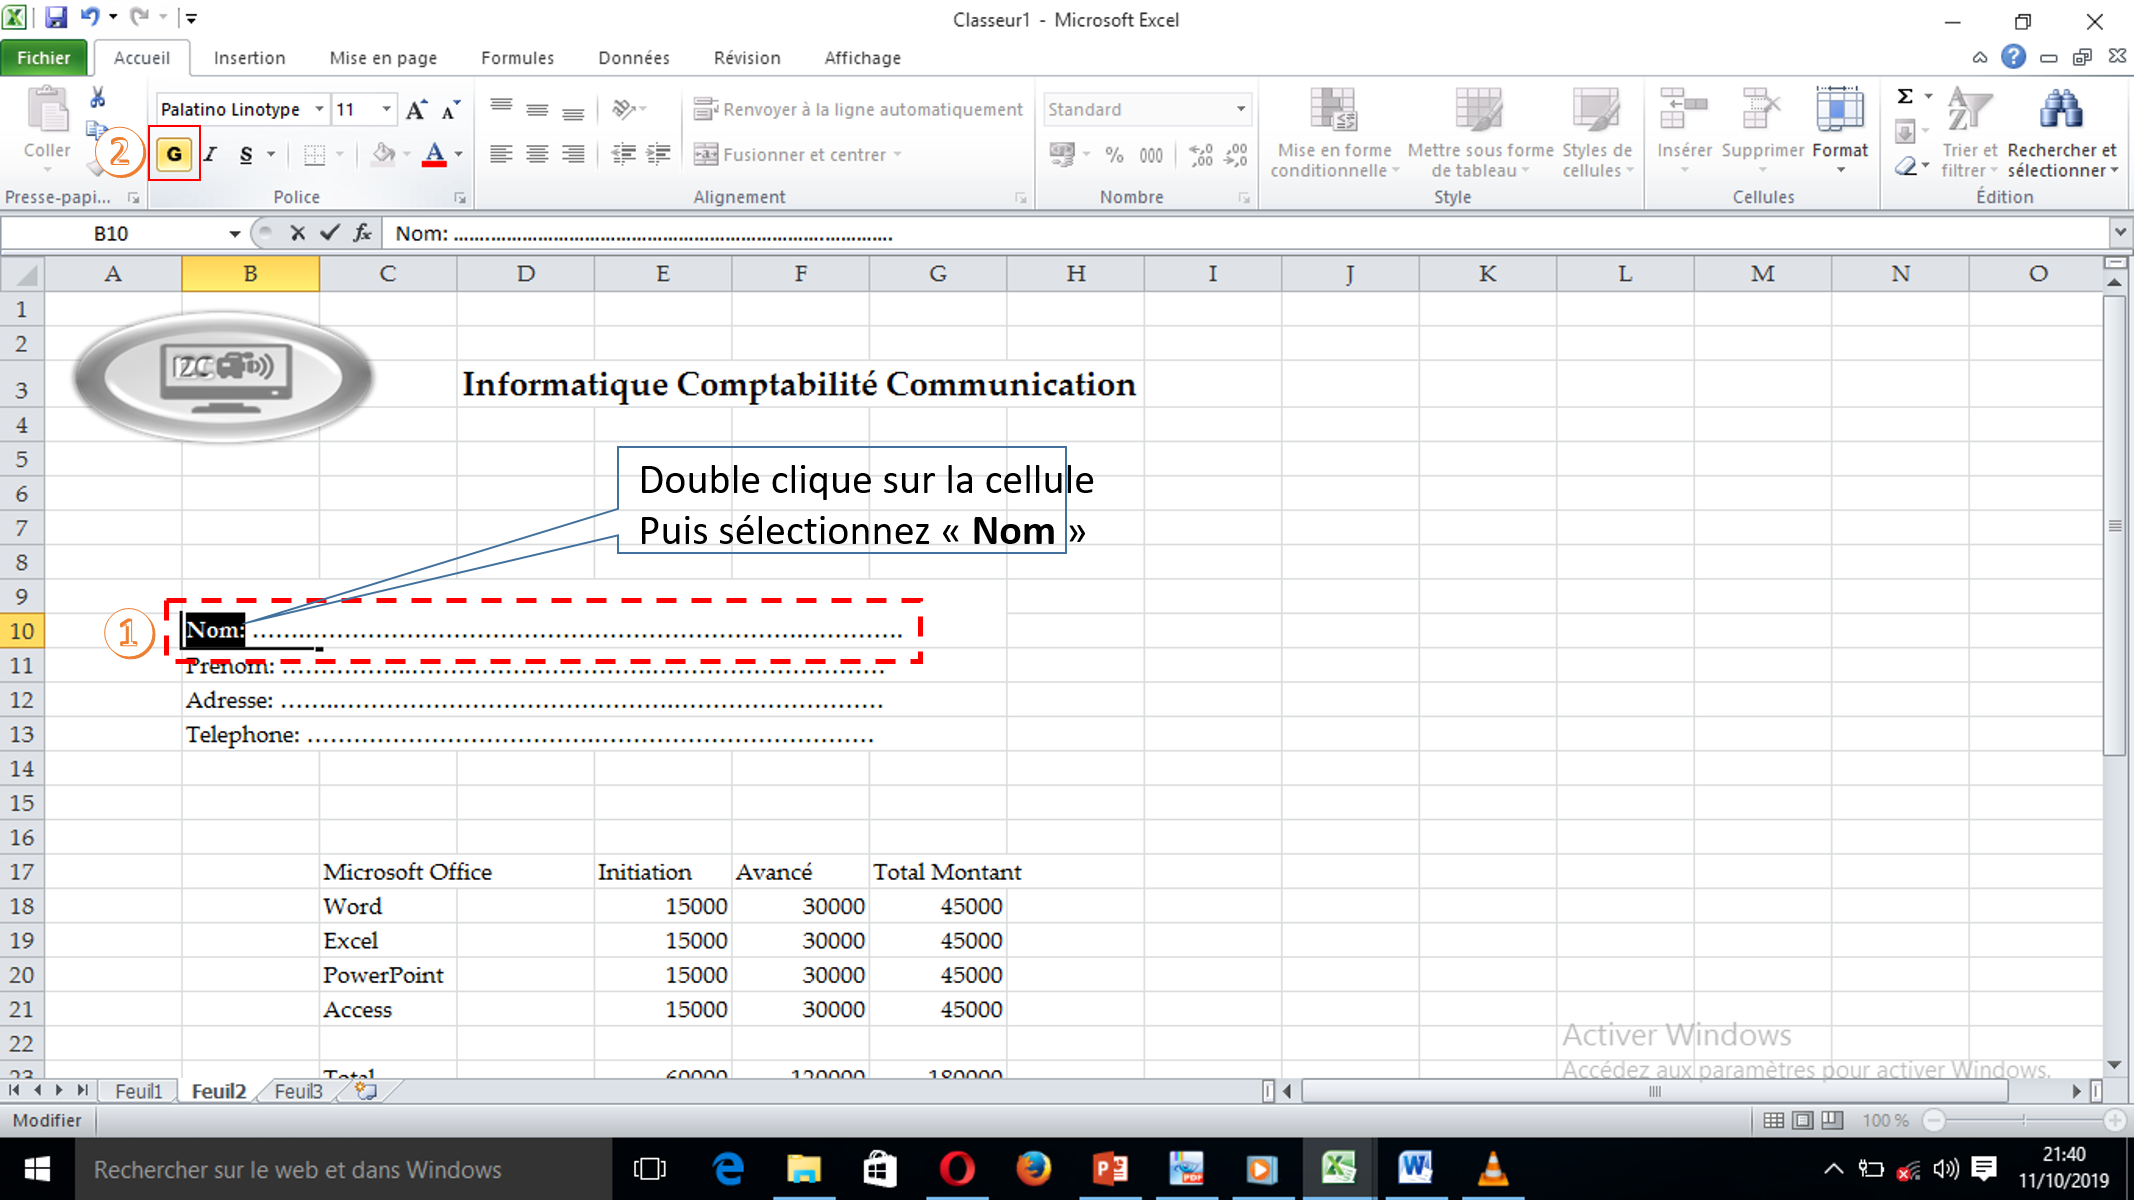
\includegraphics[ width=\linewidth,height=0.705\paperheight]{img/17}
\end{landscape}
\begin{landscape} 		
	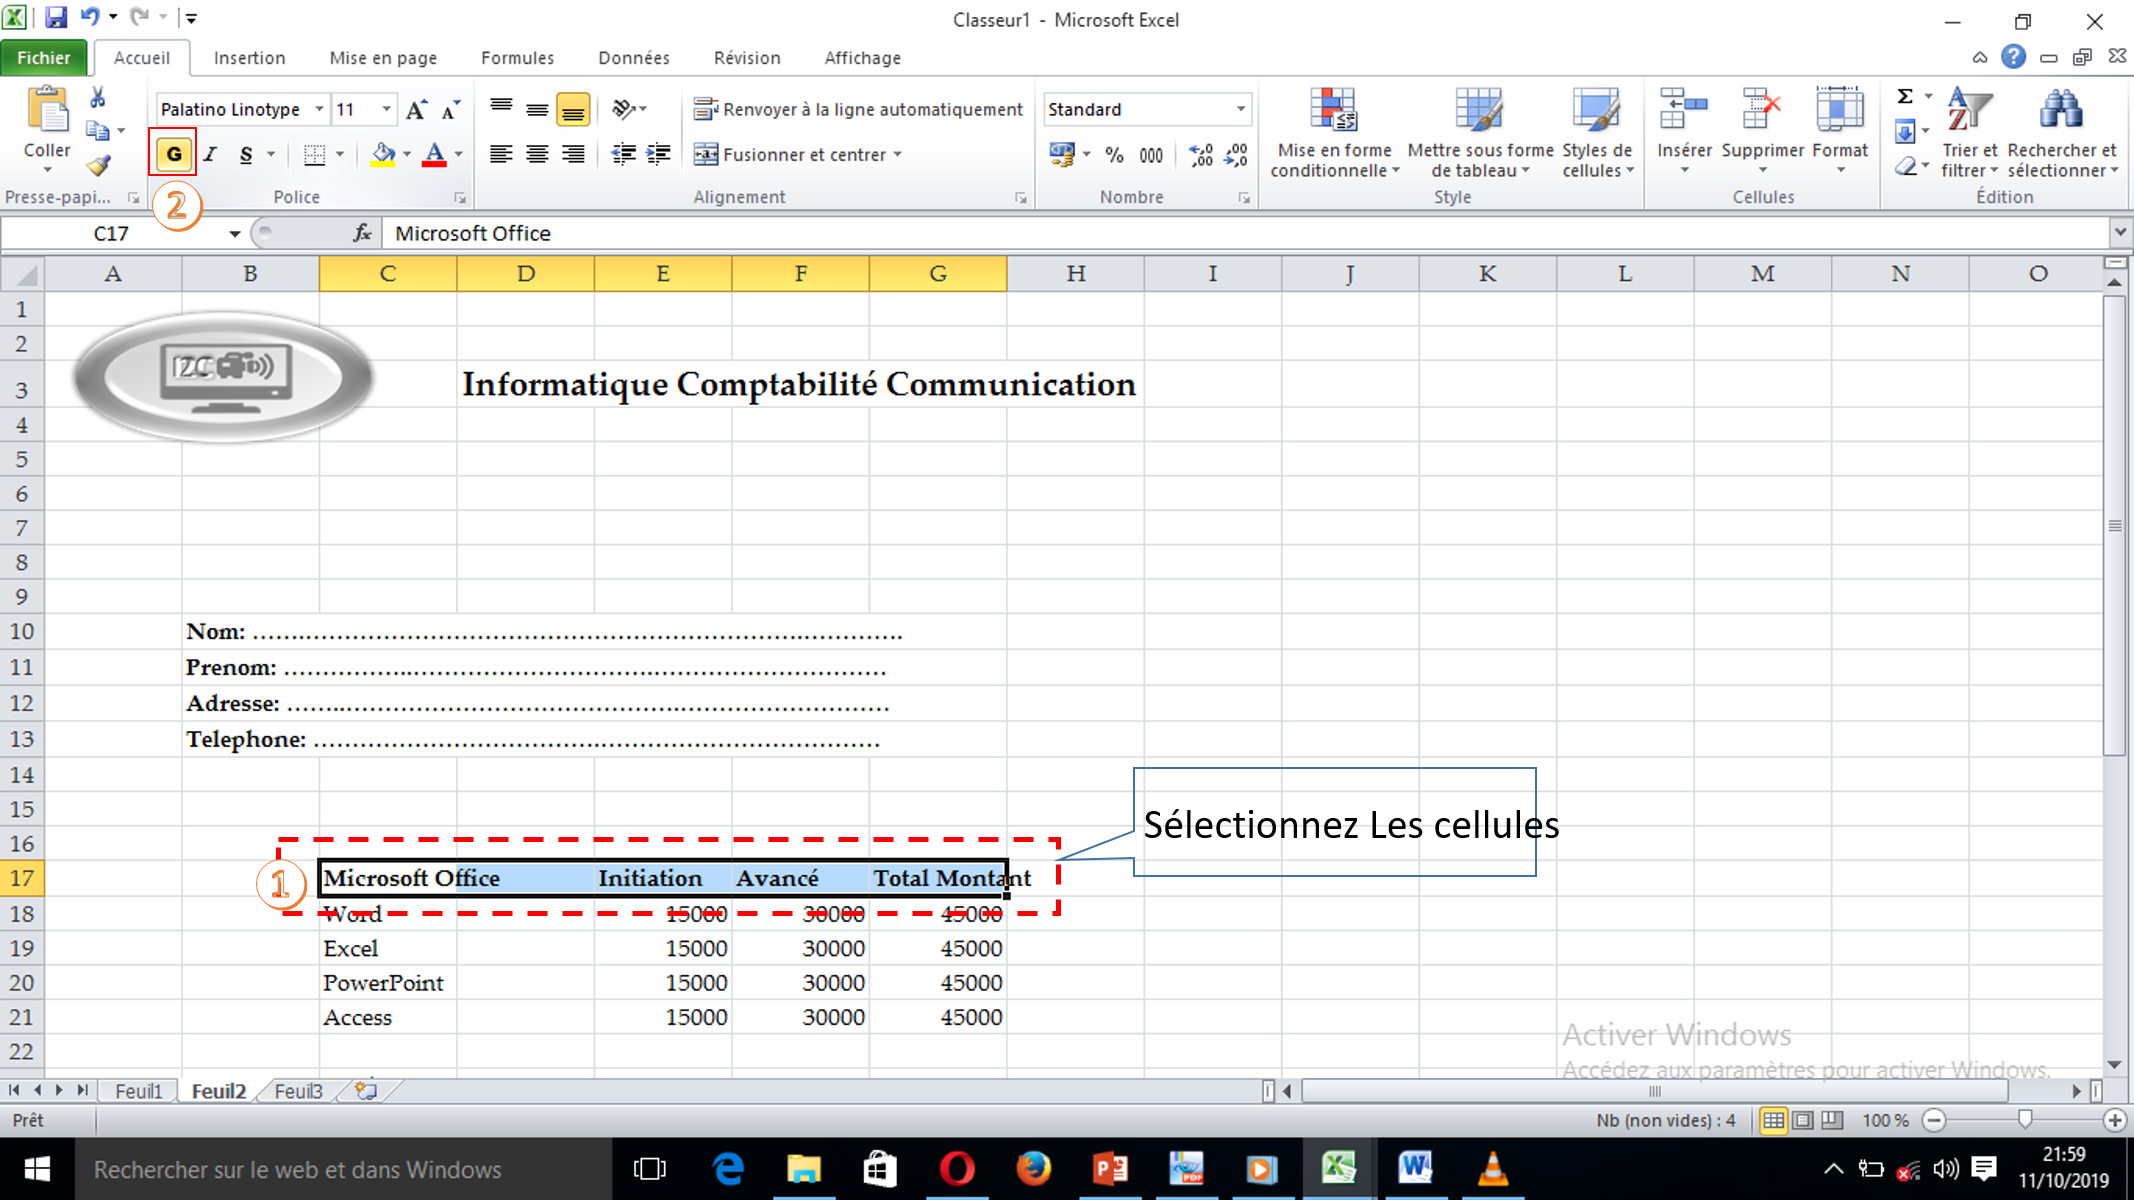
\includegraphics[ width=\linewidth,height=0.705\paperheight]{img/18}
\end{landscape}
\begin{landscape} 		
	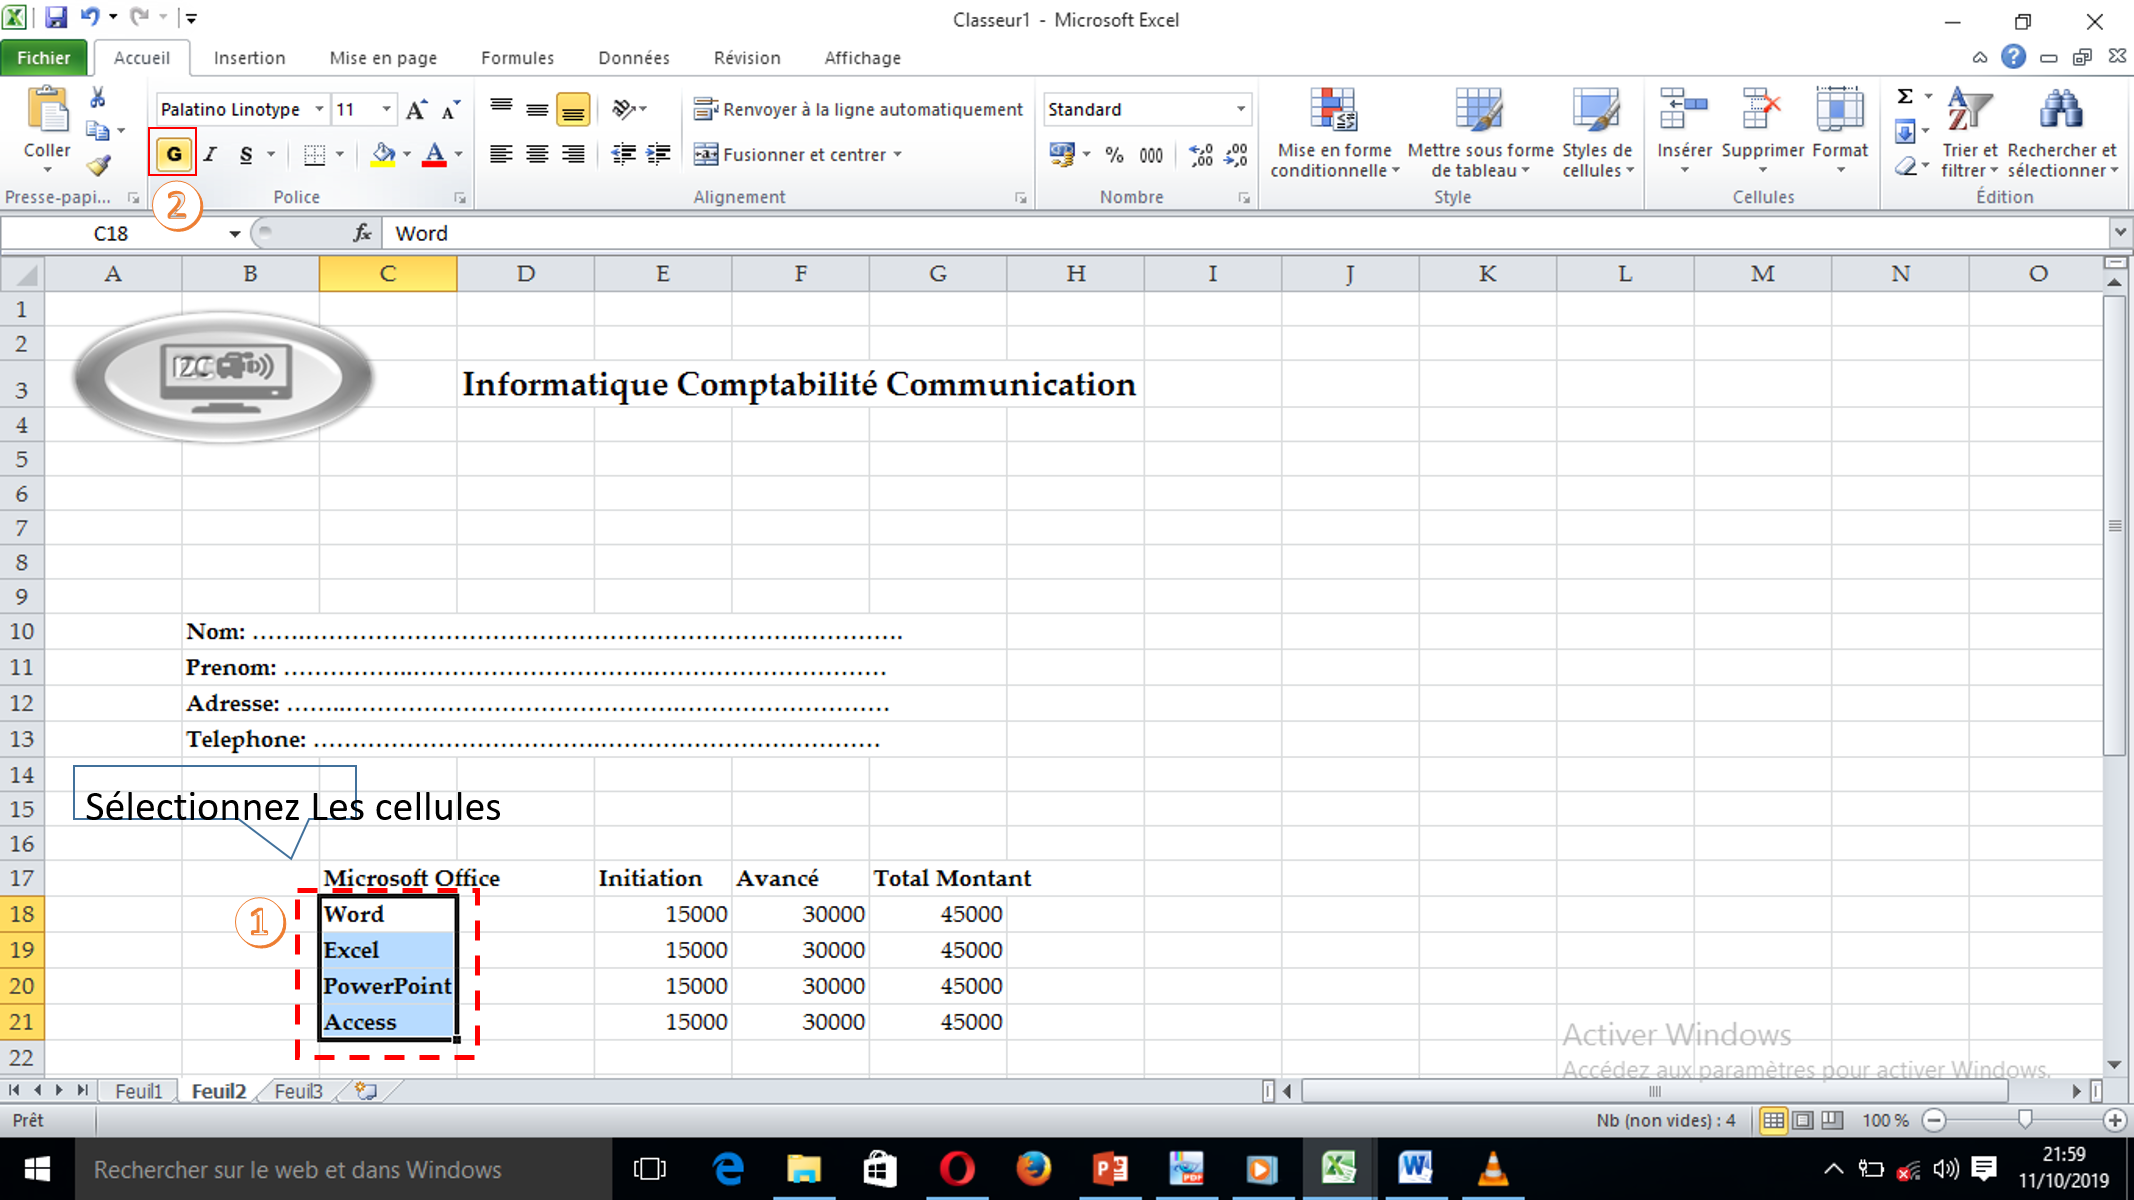
\includegraphics[ width=\linewidth,height=0.705\paperheight]{img/19}
\end{landscape}
\begin{landscape} 		
	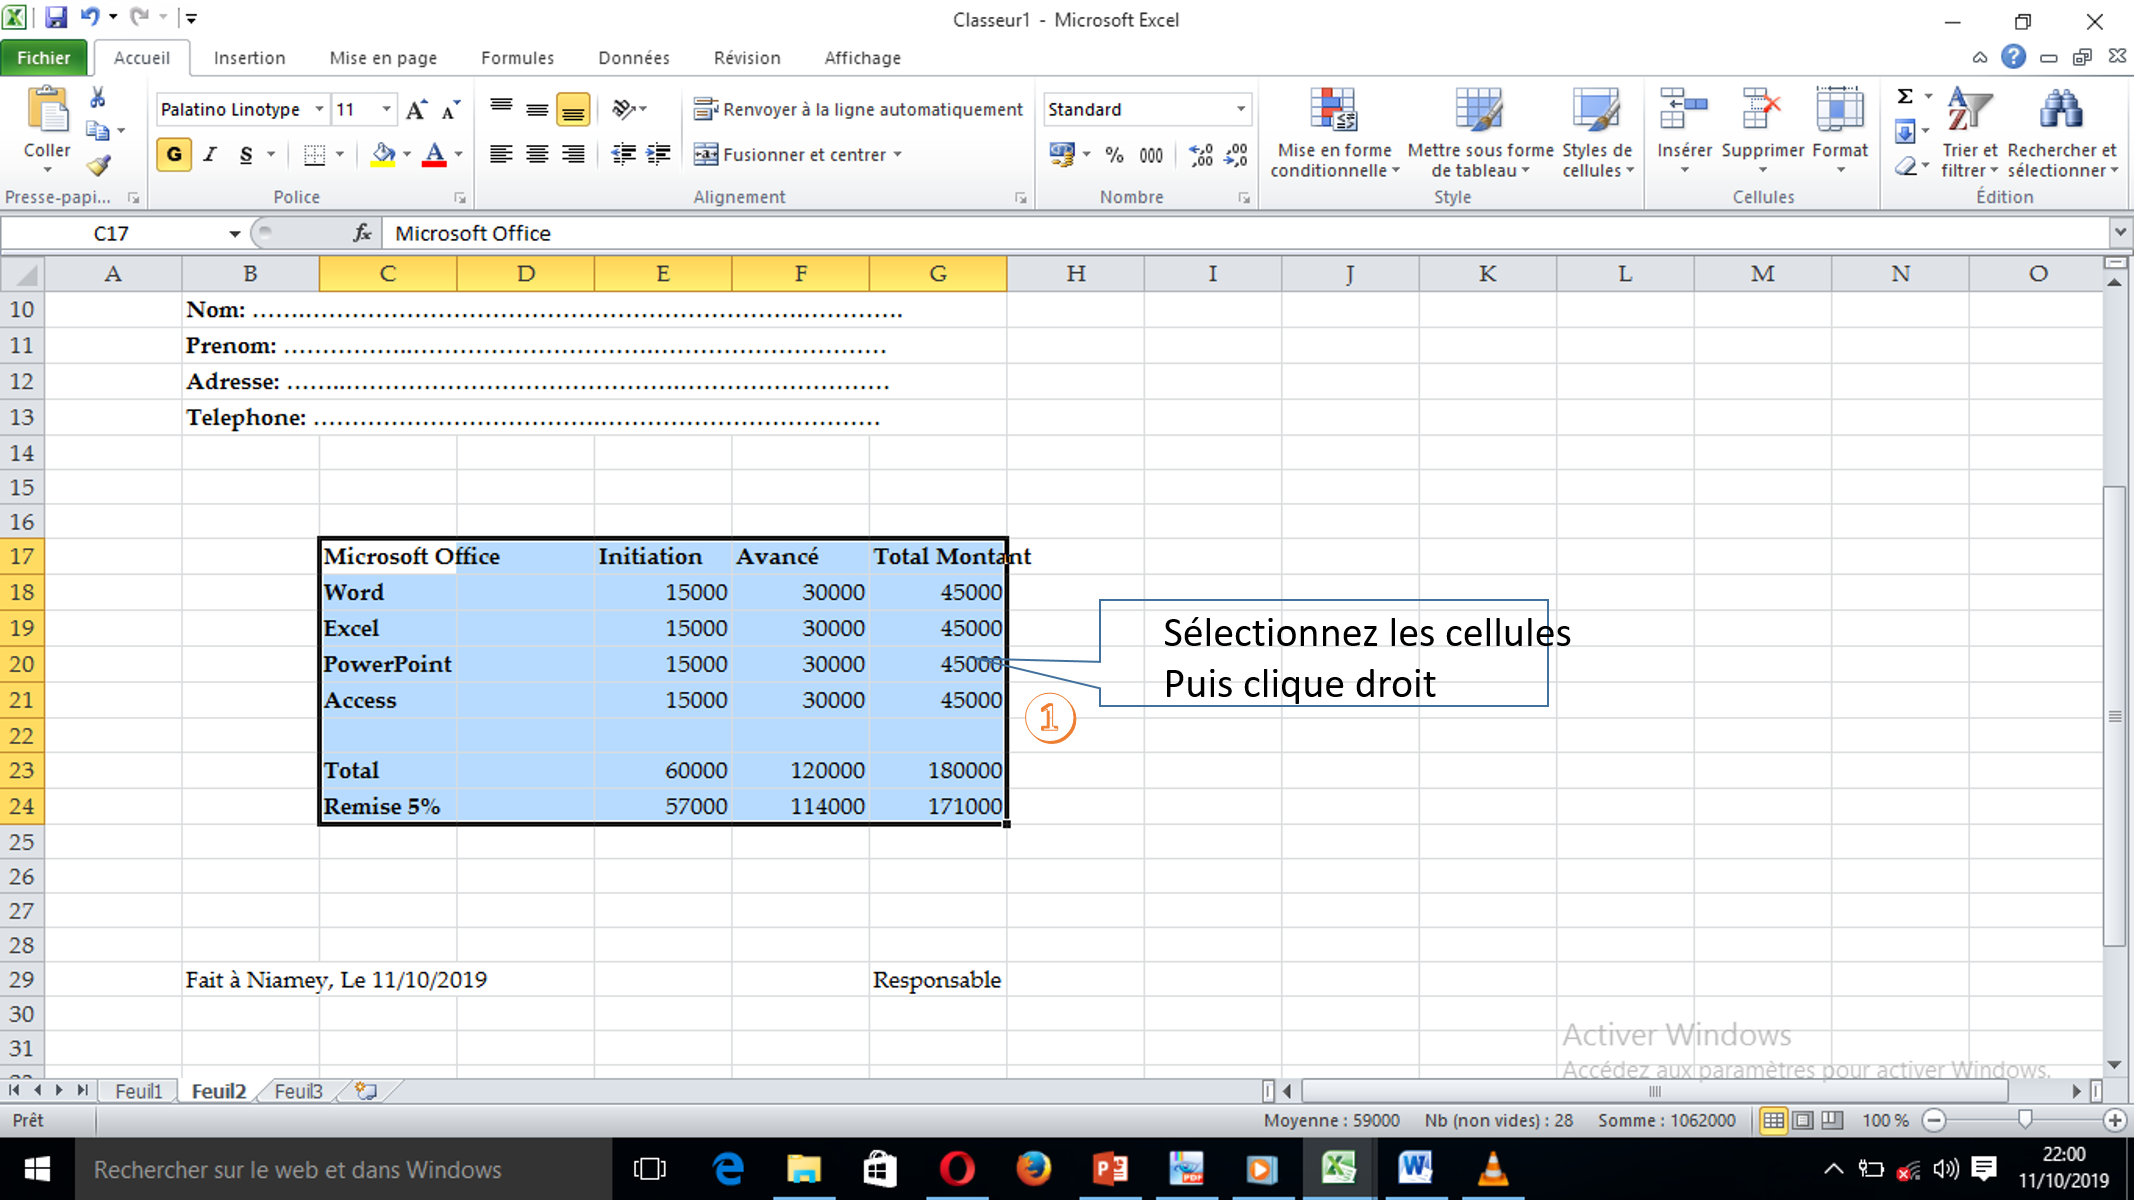
\includegraphics[ width=\linewidth,height=0.705\paperheight]{img/20}
\end{landscape}
\begin{landscape} 		
	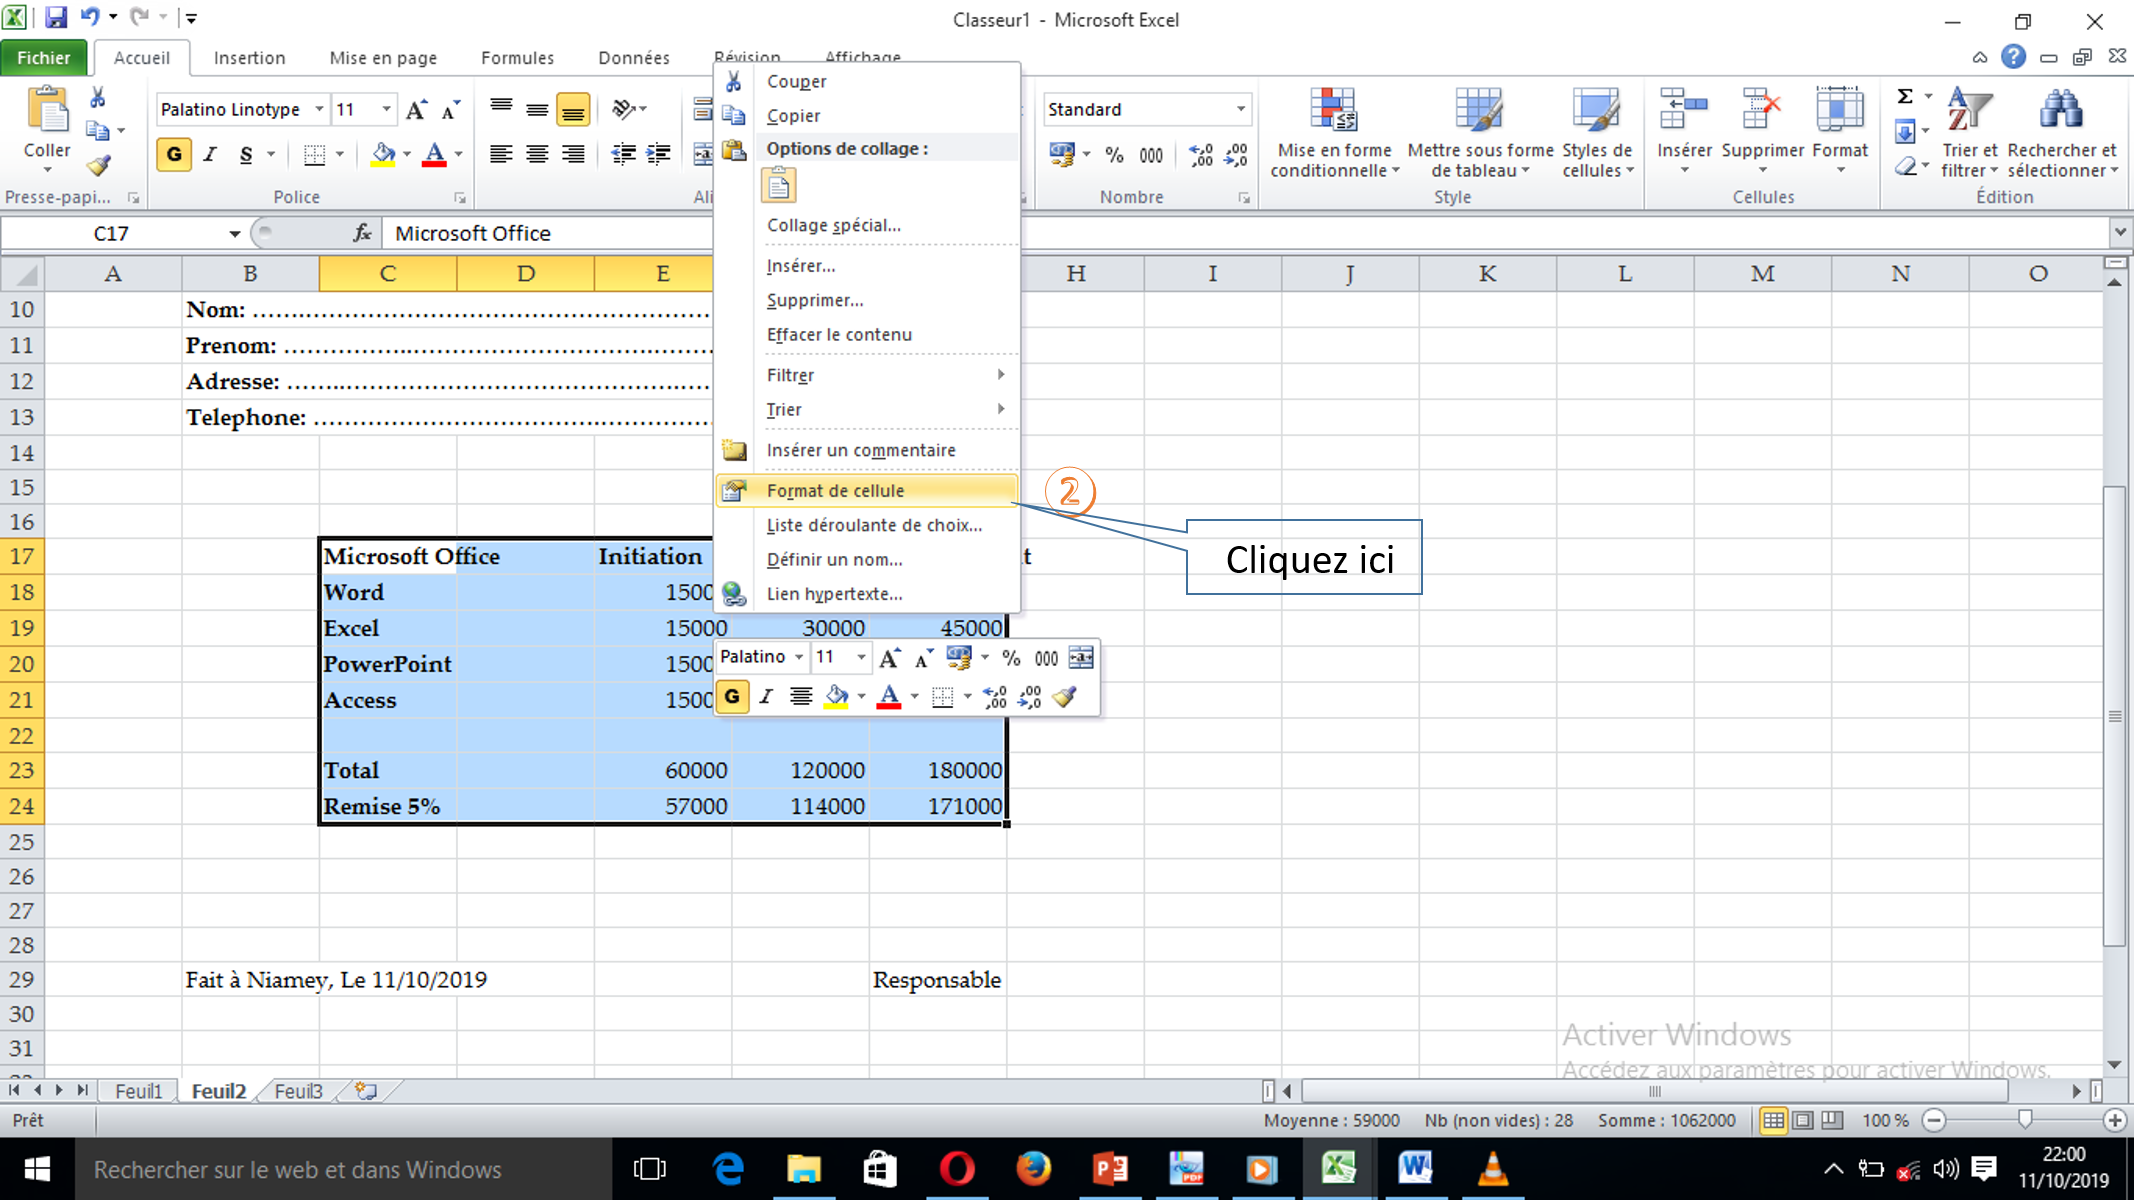
\includegraphics[ width=\linewidth,height=0.705\paperheight]{img/21}
\end{landscape}
\begin{landscape} 		
	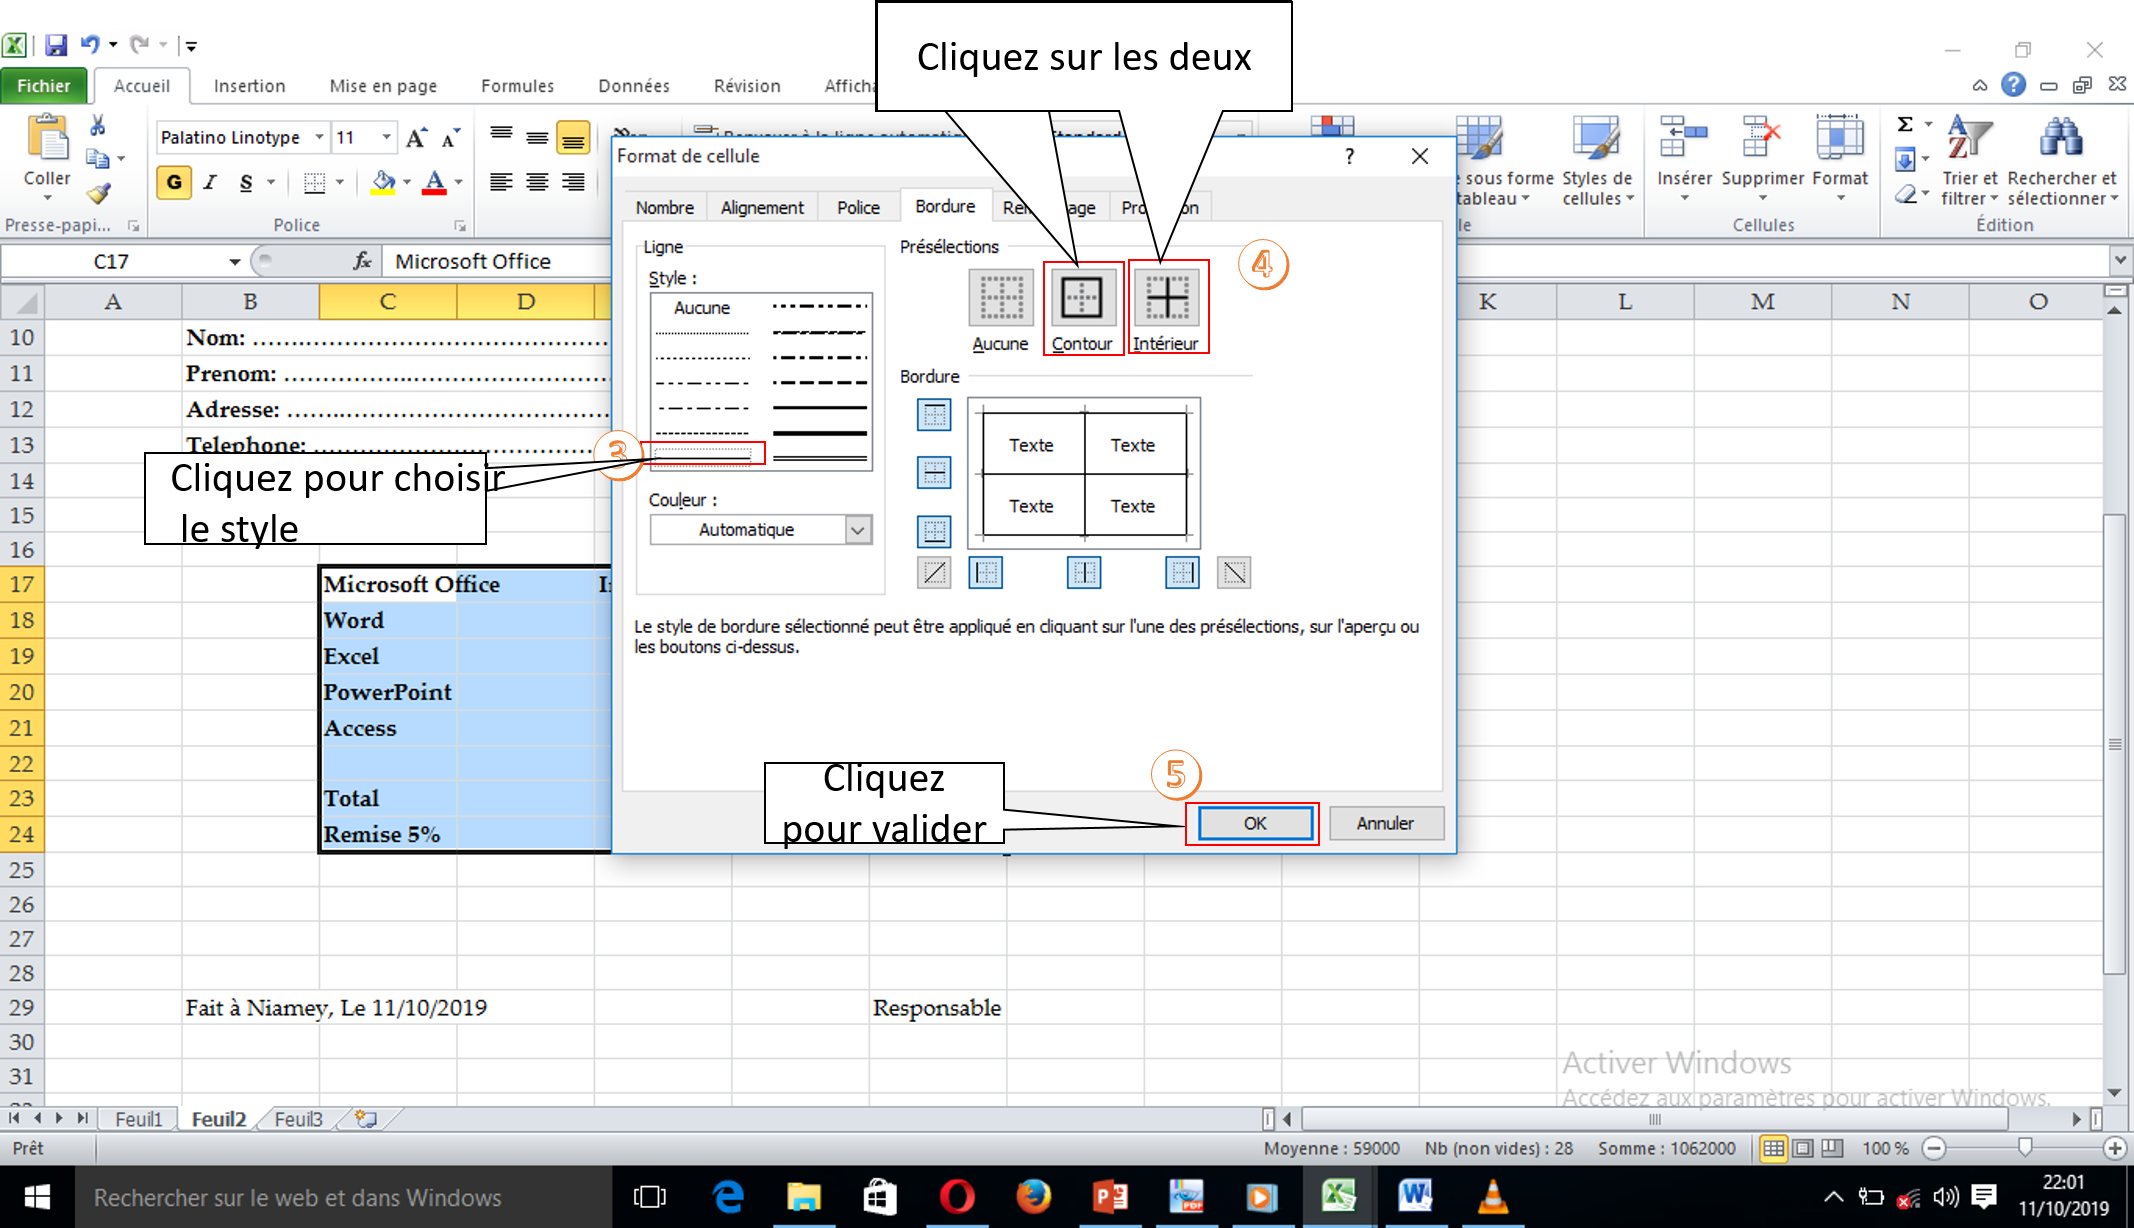
\includegraphics[ width=\linewidth,height=0.705\paperheight]{img/22}
\end{landscape}
\begin{landscape} 		
	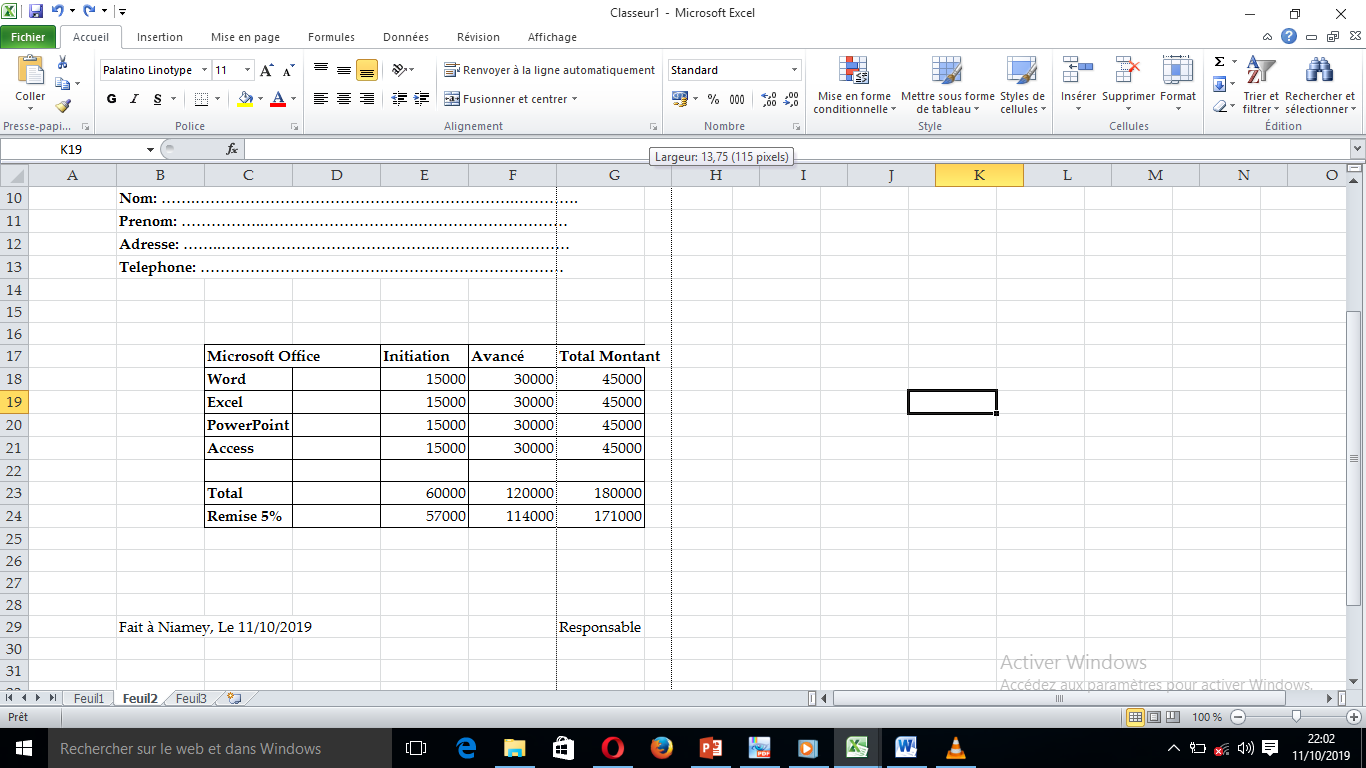
\includegraphics[ width=\linewidth,height=0.705\paperheight]{img/23}
\end{landscape}
\begin{landscape} 		
	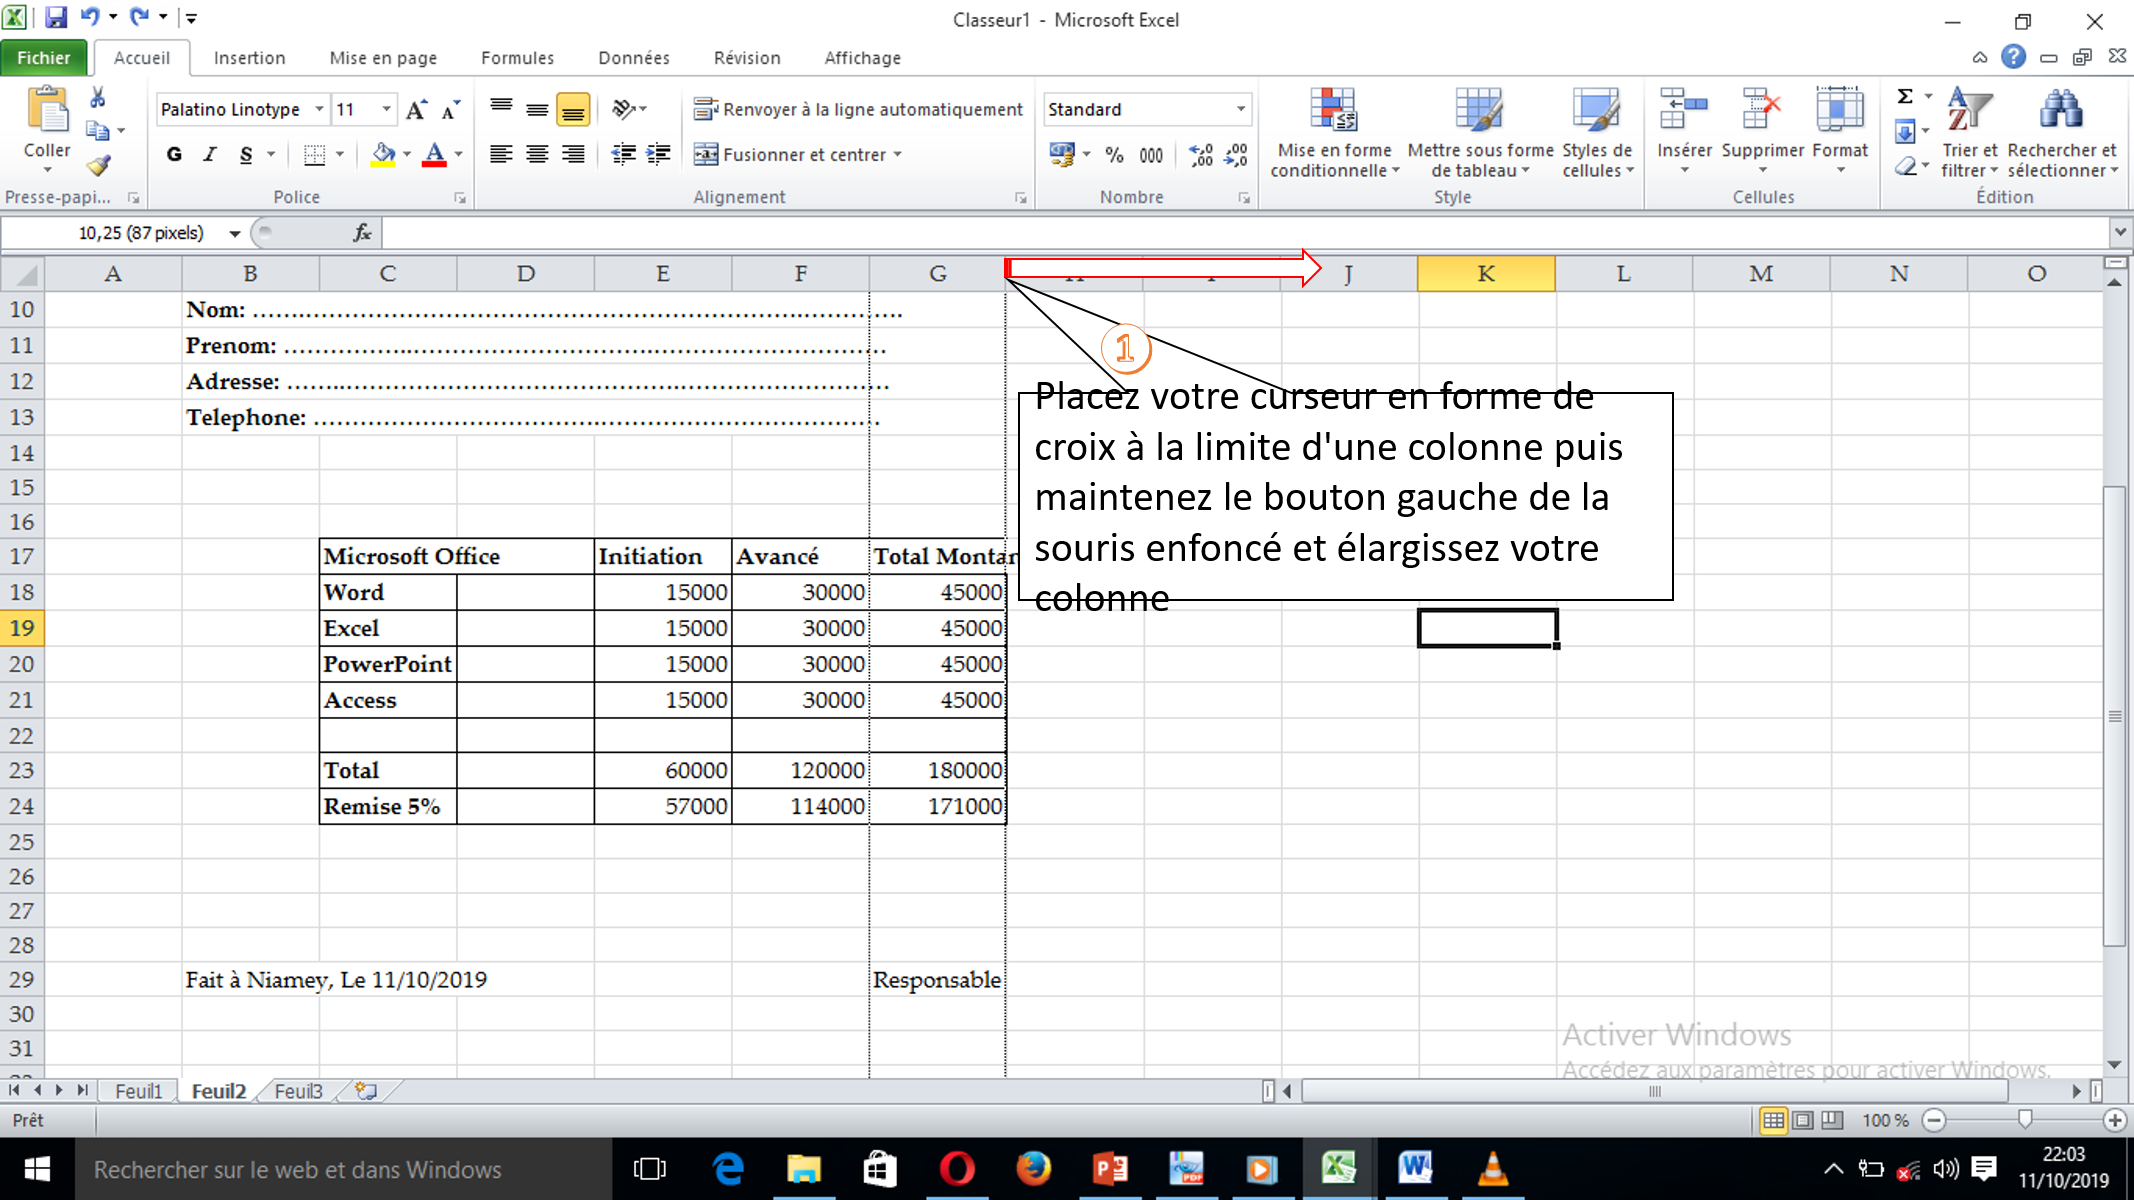
\includegraphics[ width=\linewidth,height=0.705\paperheight]{img/24}
\end{landscape}
\begin{landscape} 		
	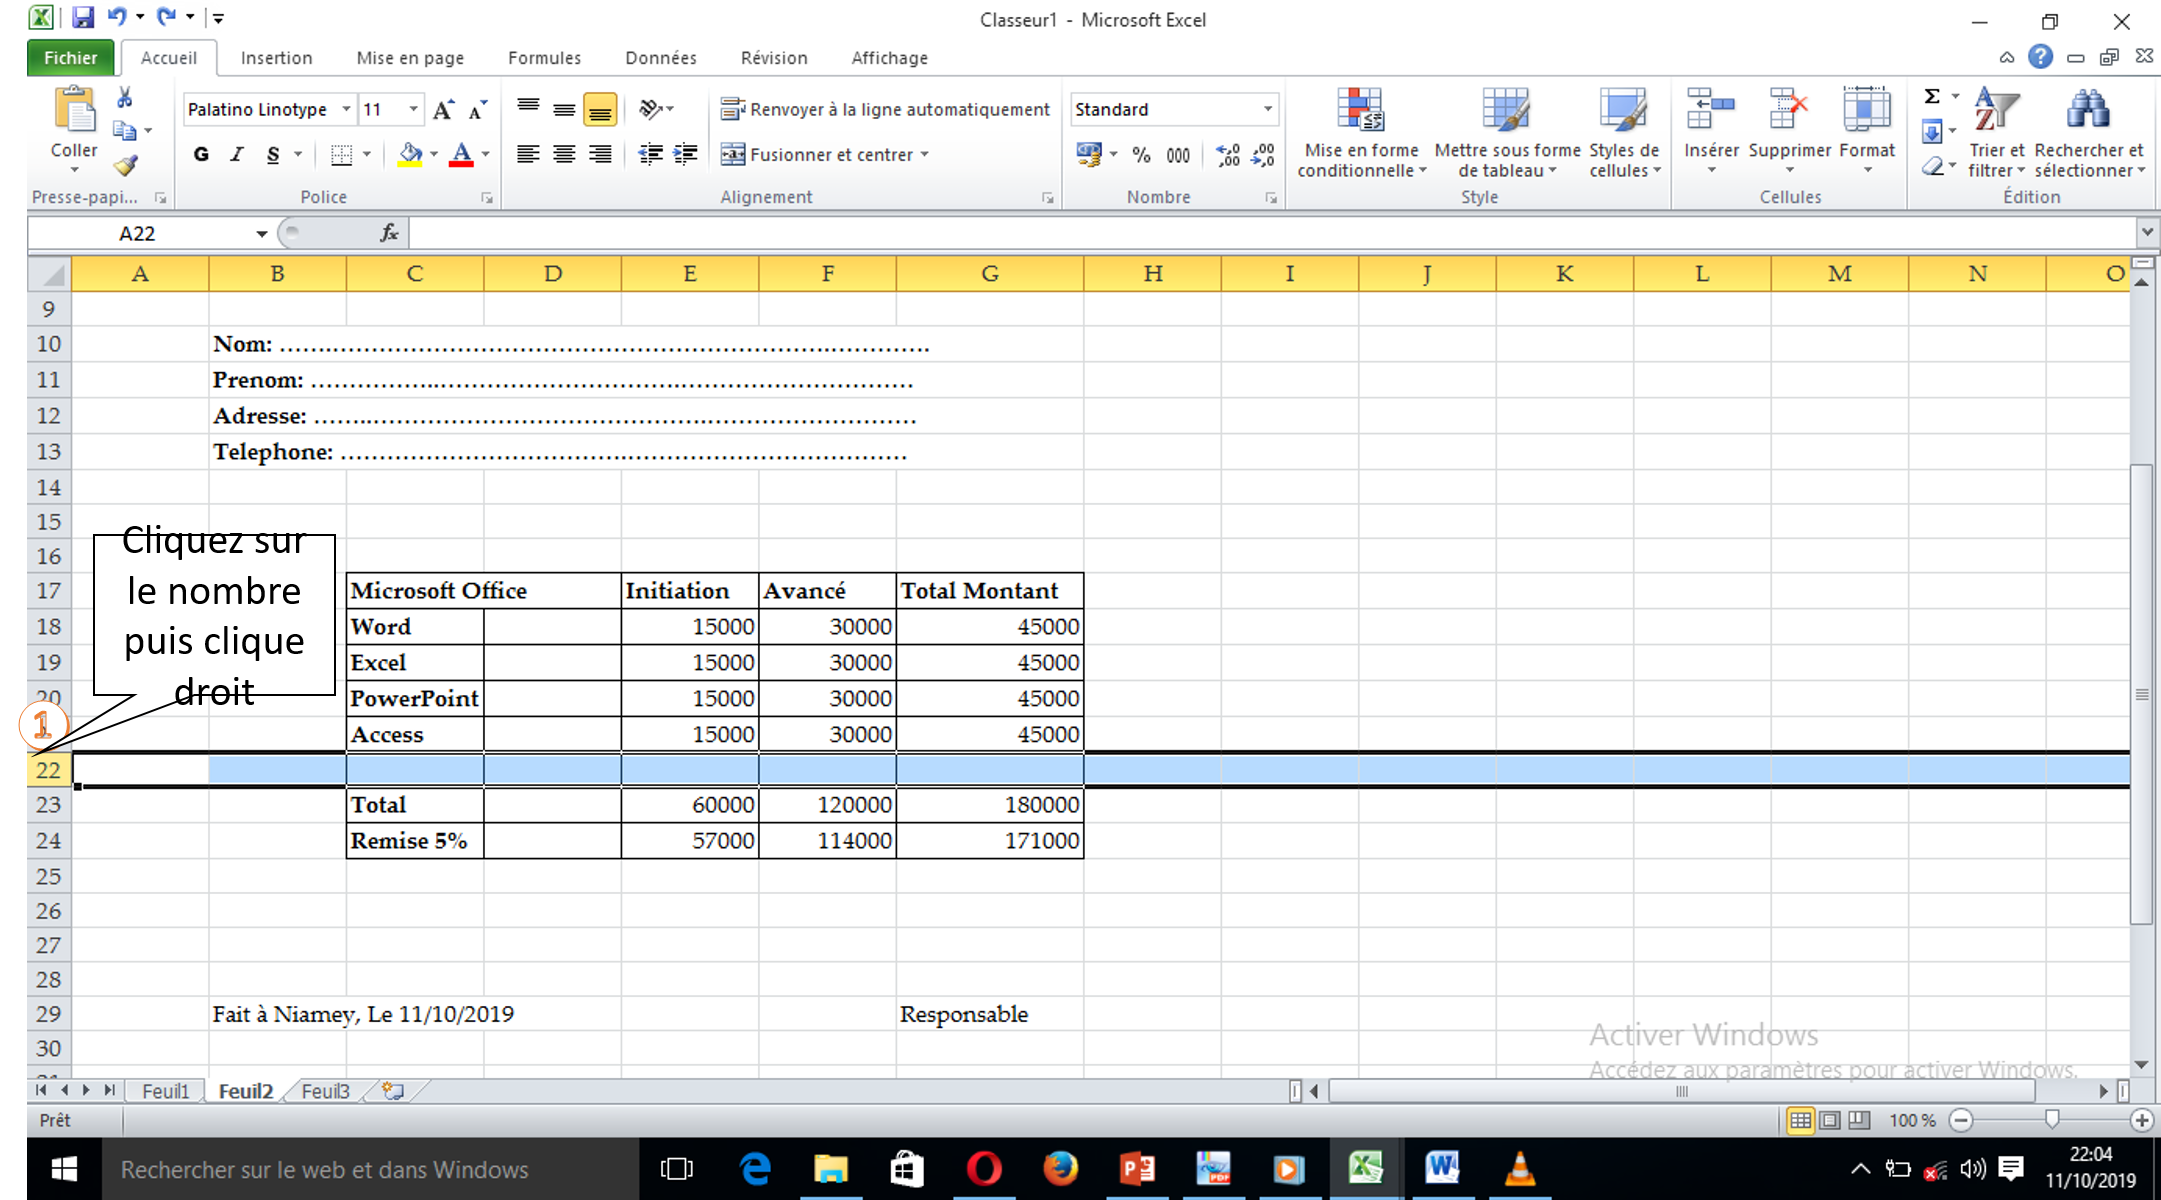
\includegraphics[ width=\linewidth,height=0.705\paperheight]{img/25}
\end{landscape}
\begin{landscape} 		
	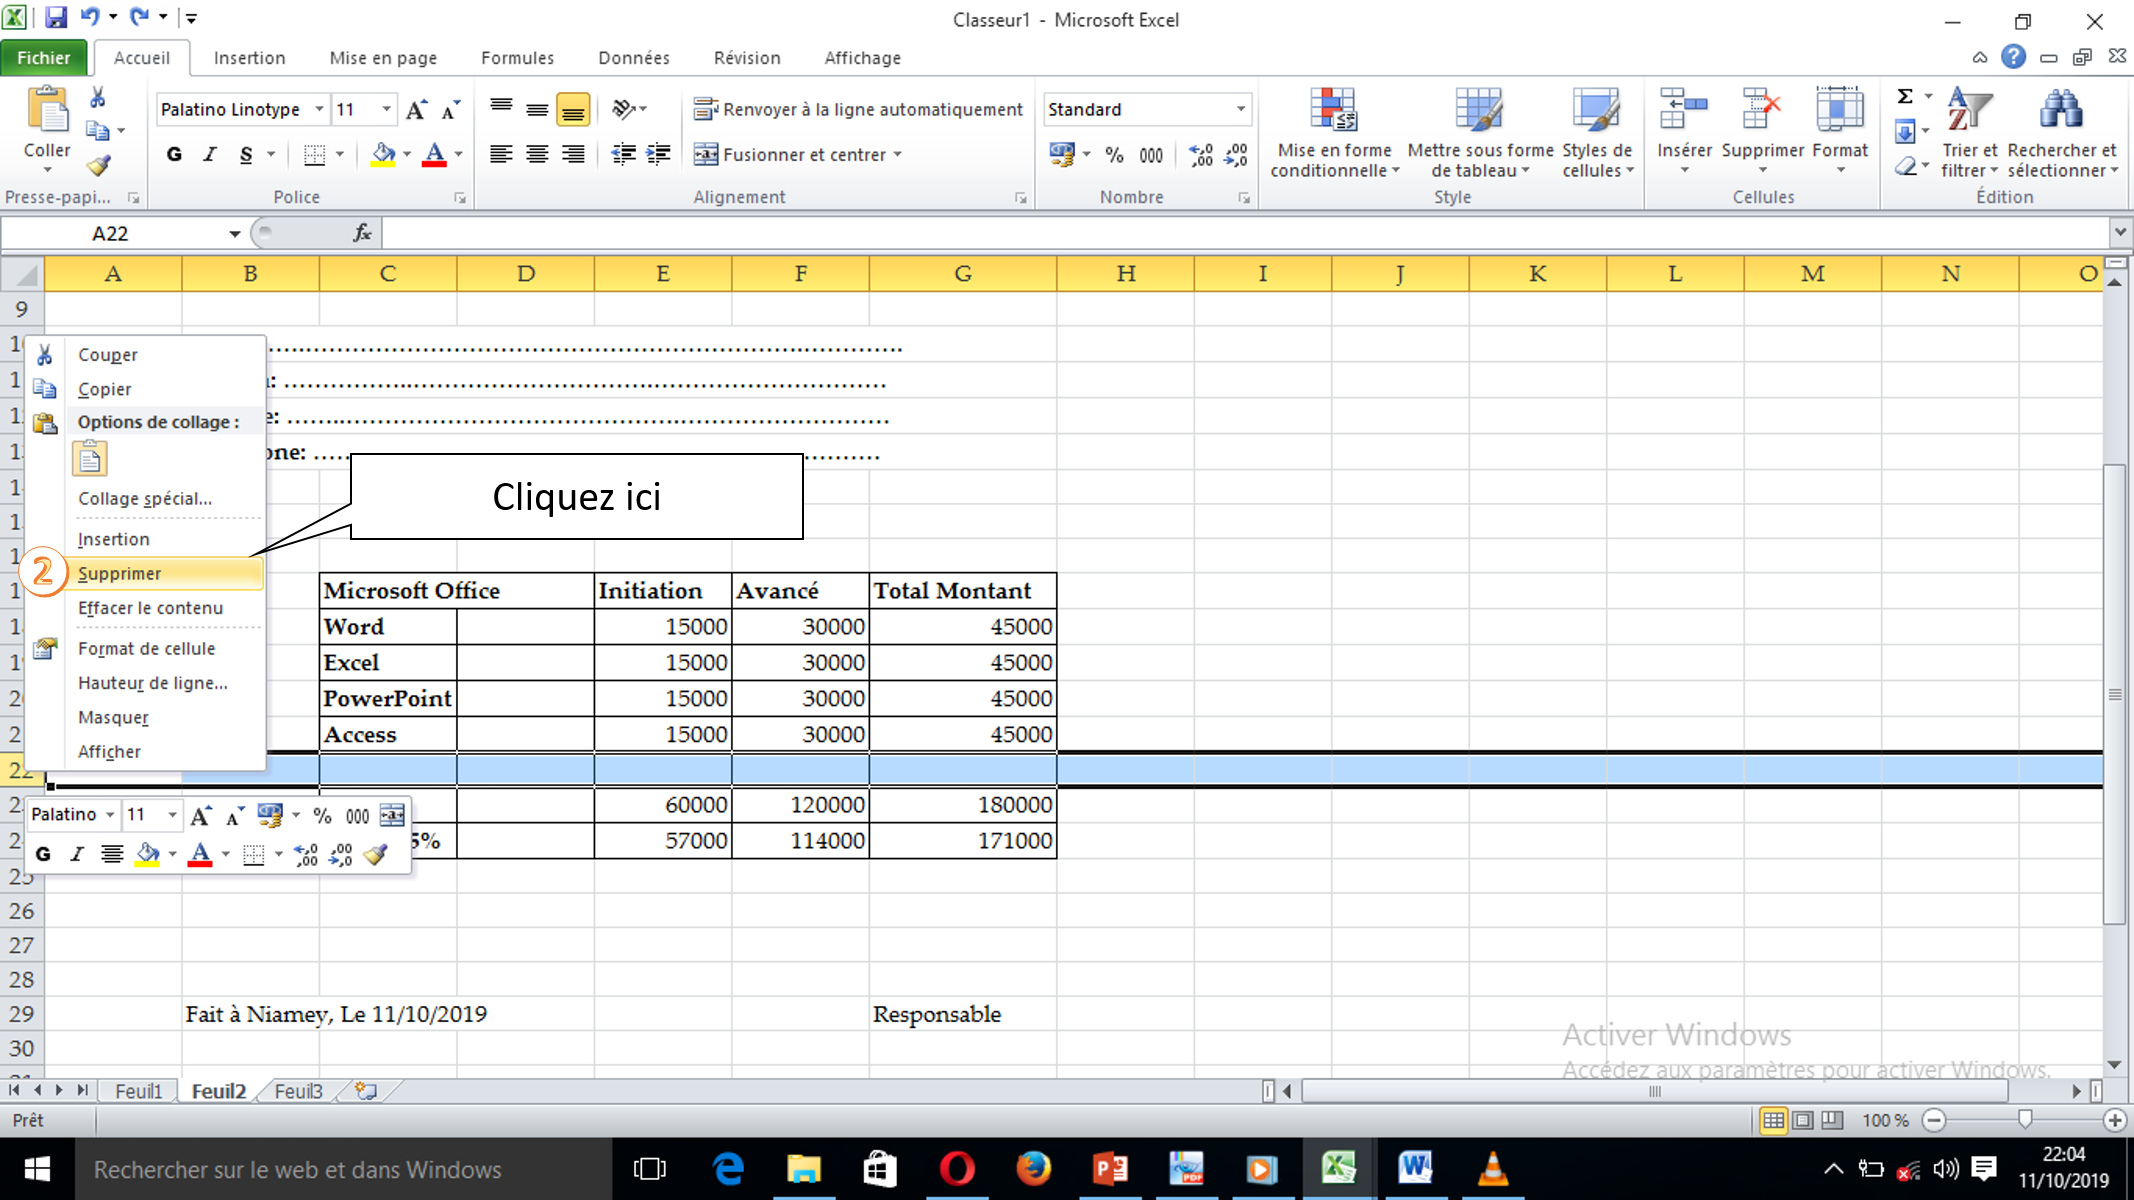
\includegraphics[ width=\linewidth,height=0.705\paperheight]{img/26}
\end{landscape}
\begin{landscape} 		
	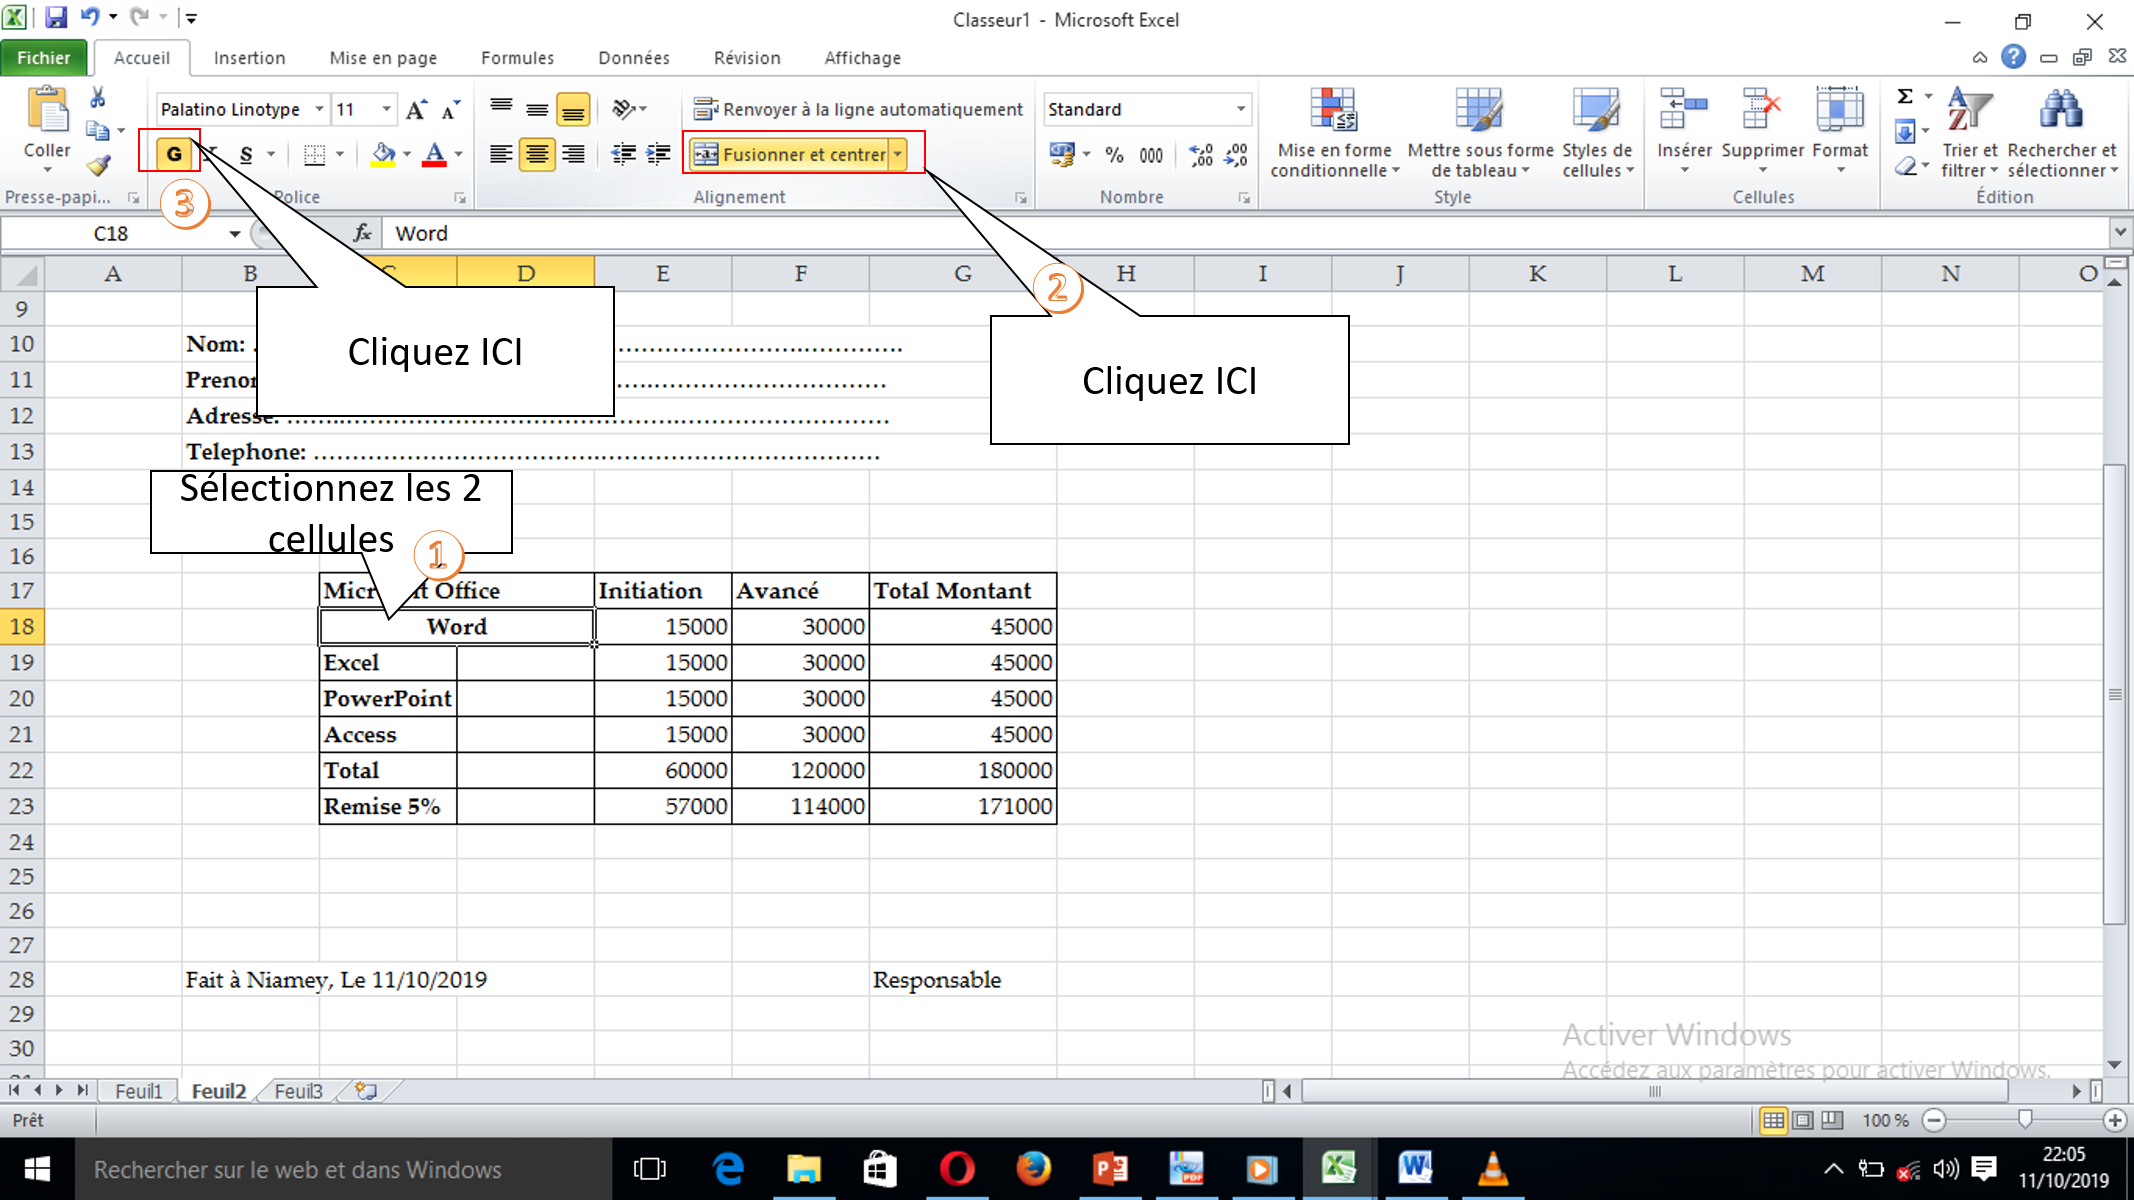
\includegraphics[ width=\linewidth,height=0.705\paperheight]{img/27}
\end{landscape}
\begin{landscape} 		
	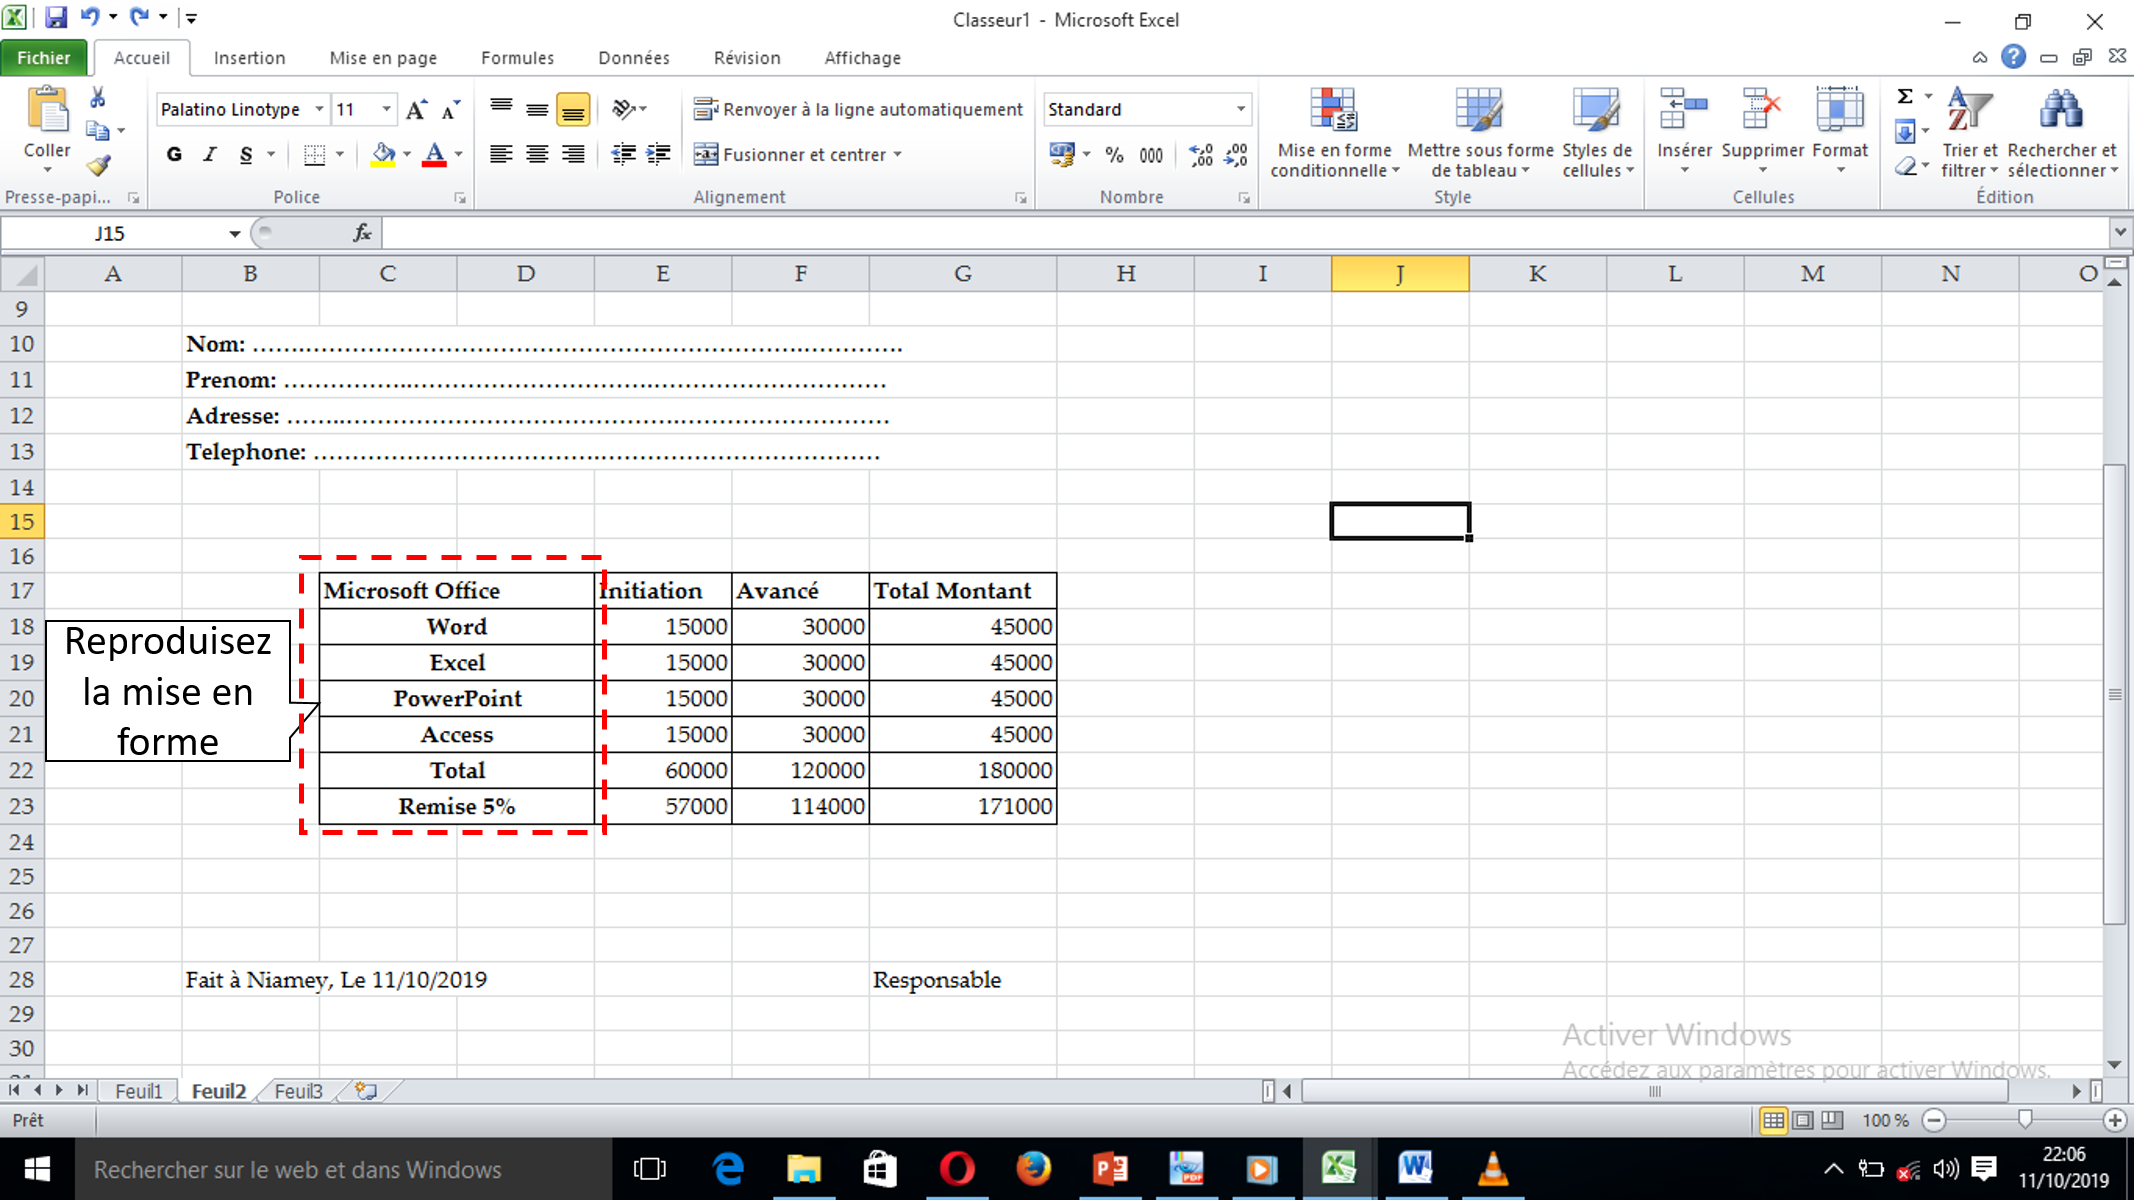
\includegraphics[ width=\linewidth,height=0.705\paperheight]{img/28}
\end{landscape}
\begin{landscape} 		
	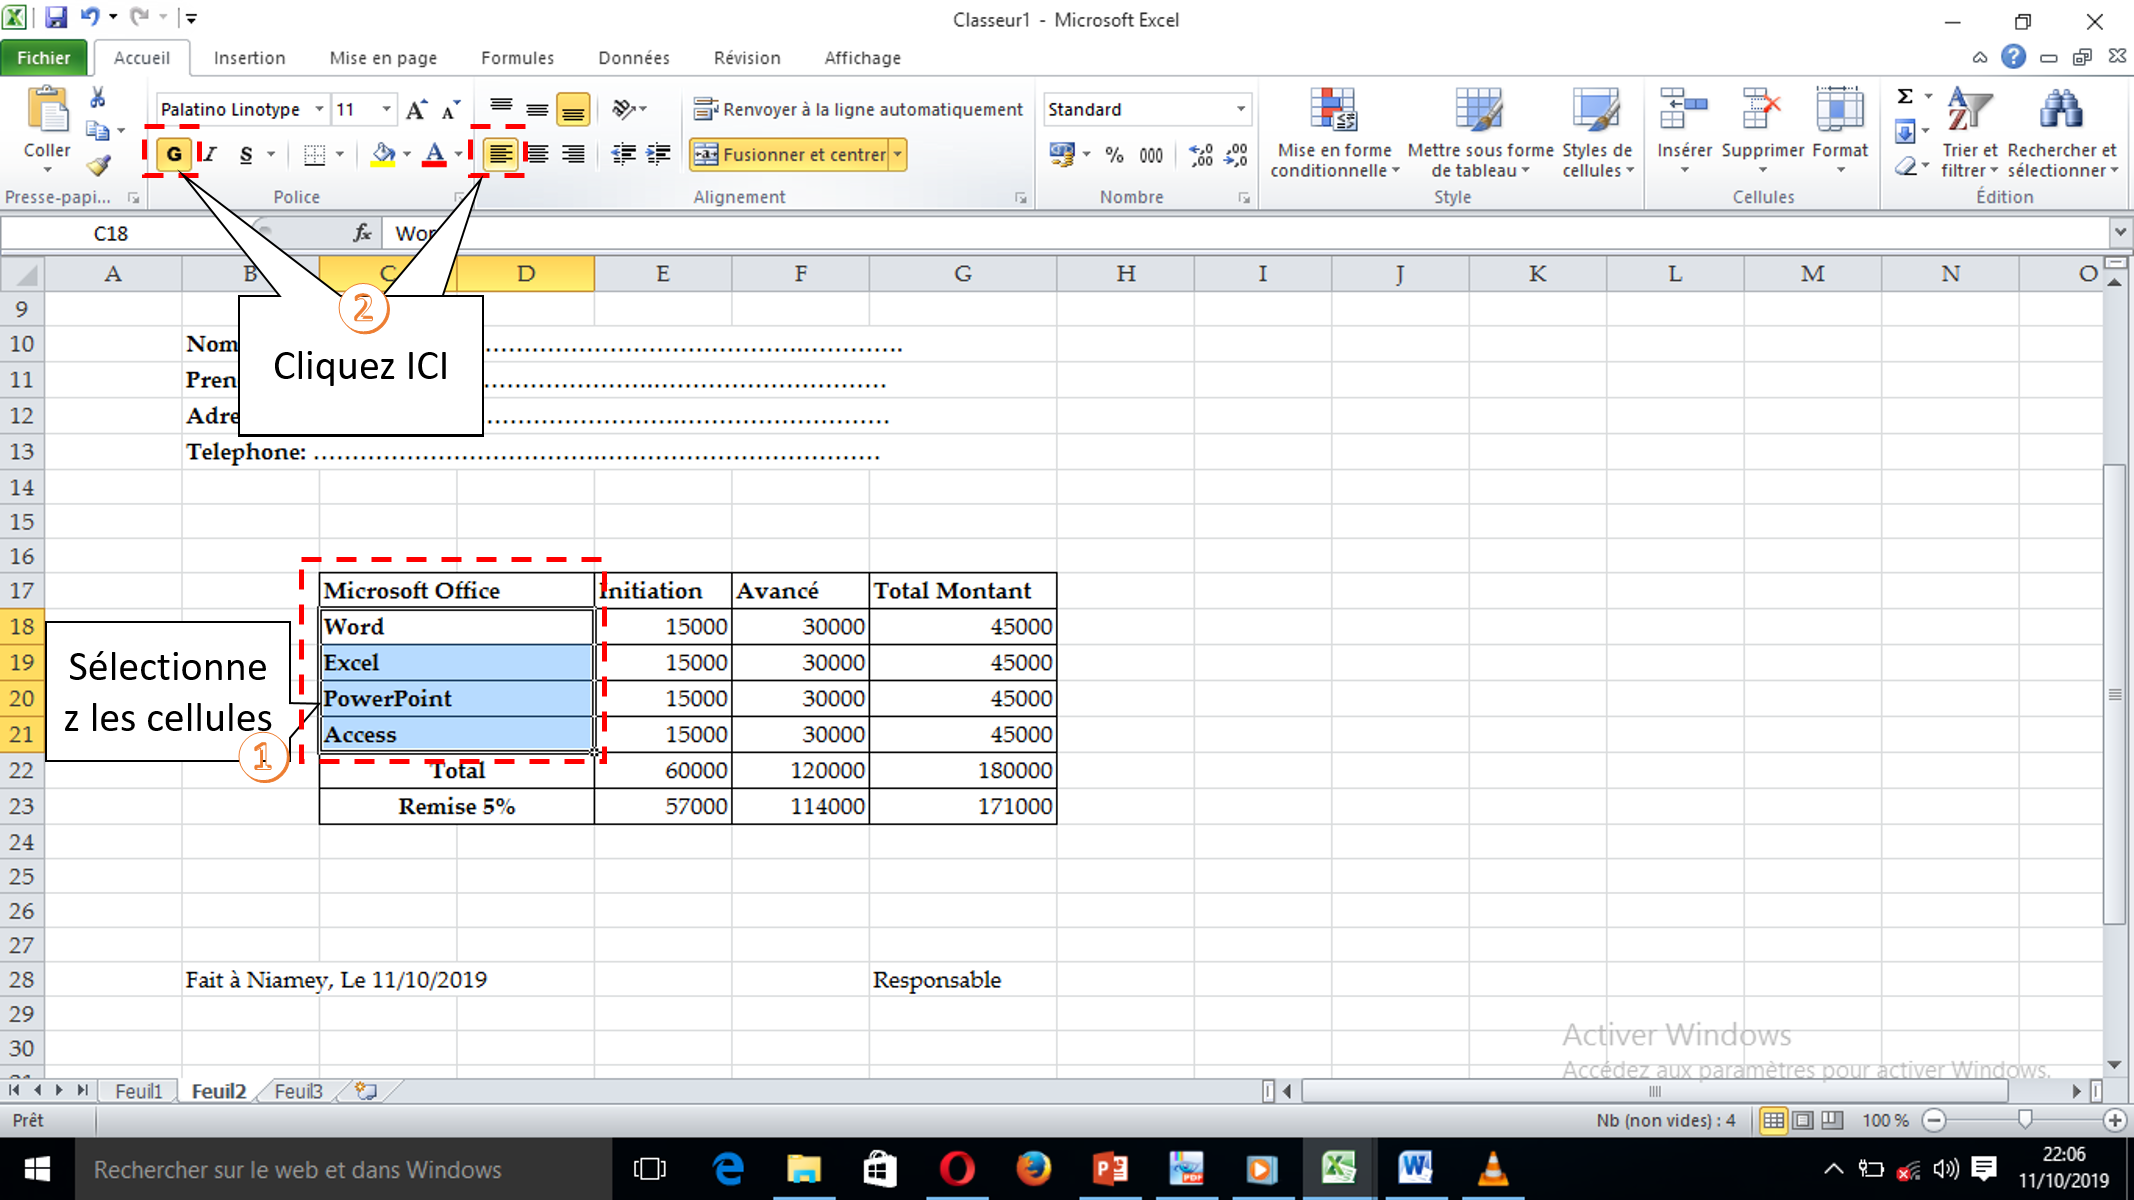
\includegraphics[ width=\linewidth,height=0.705\paperheight]{img/29}
\end{landscape}
\begin{landscape} 		
	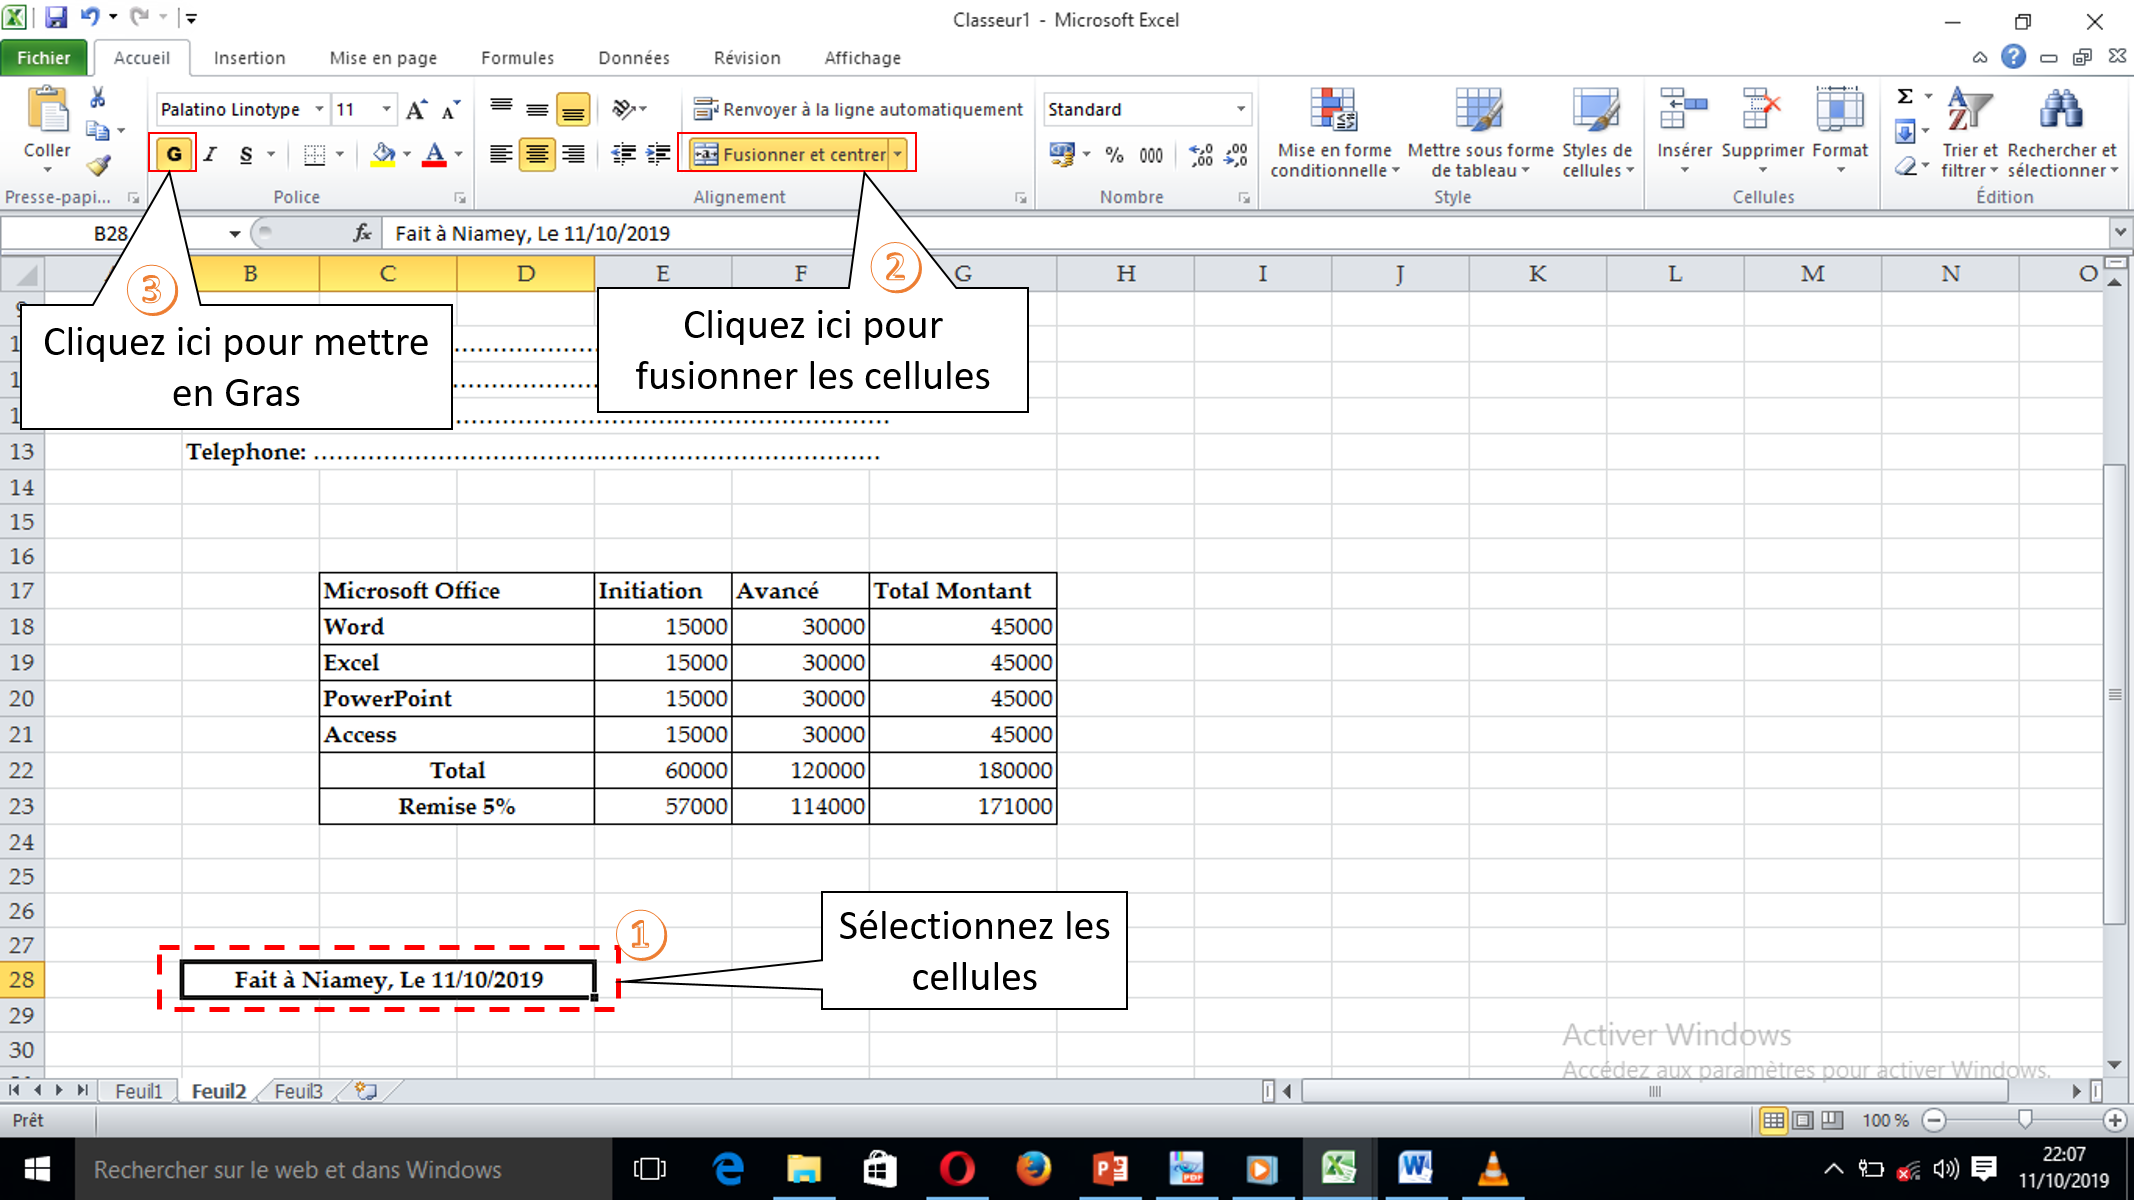
\includegraphics[ width=\linewidth,height=0.705\paperheight]{img/30}
\end{landscape}
\begin{landscape} 		
	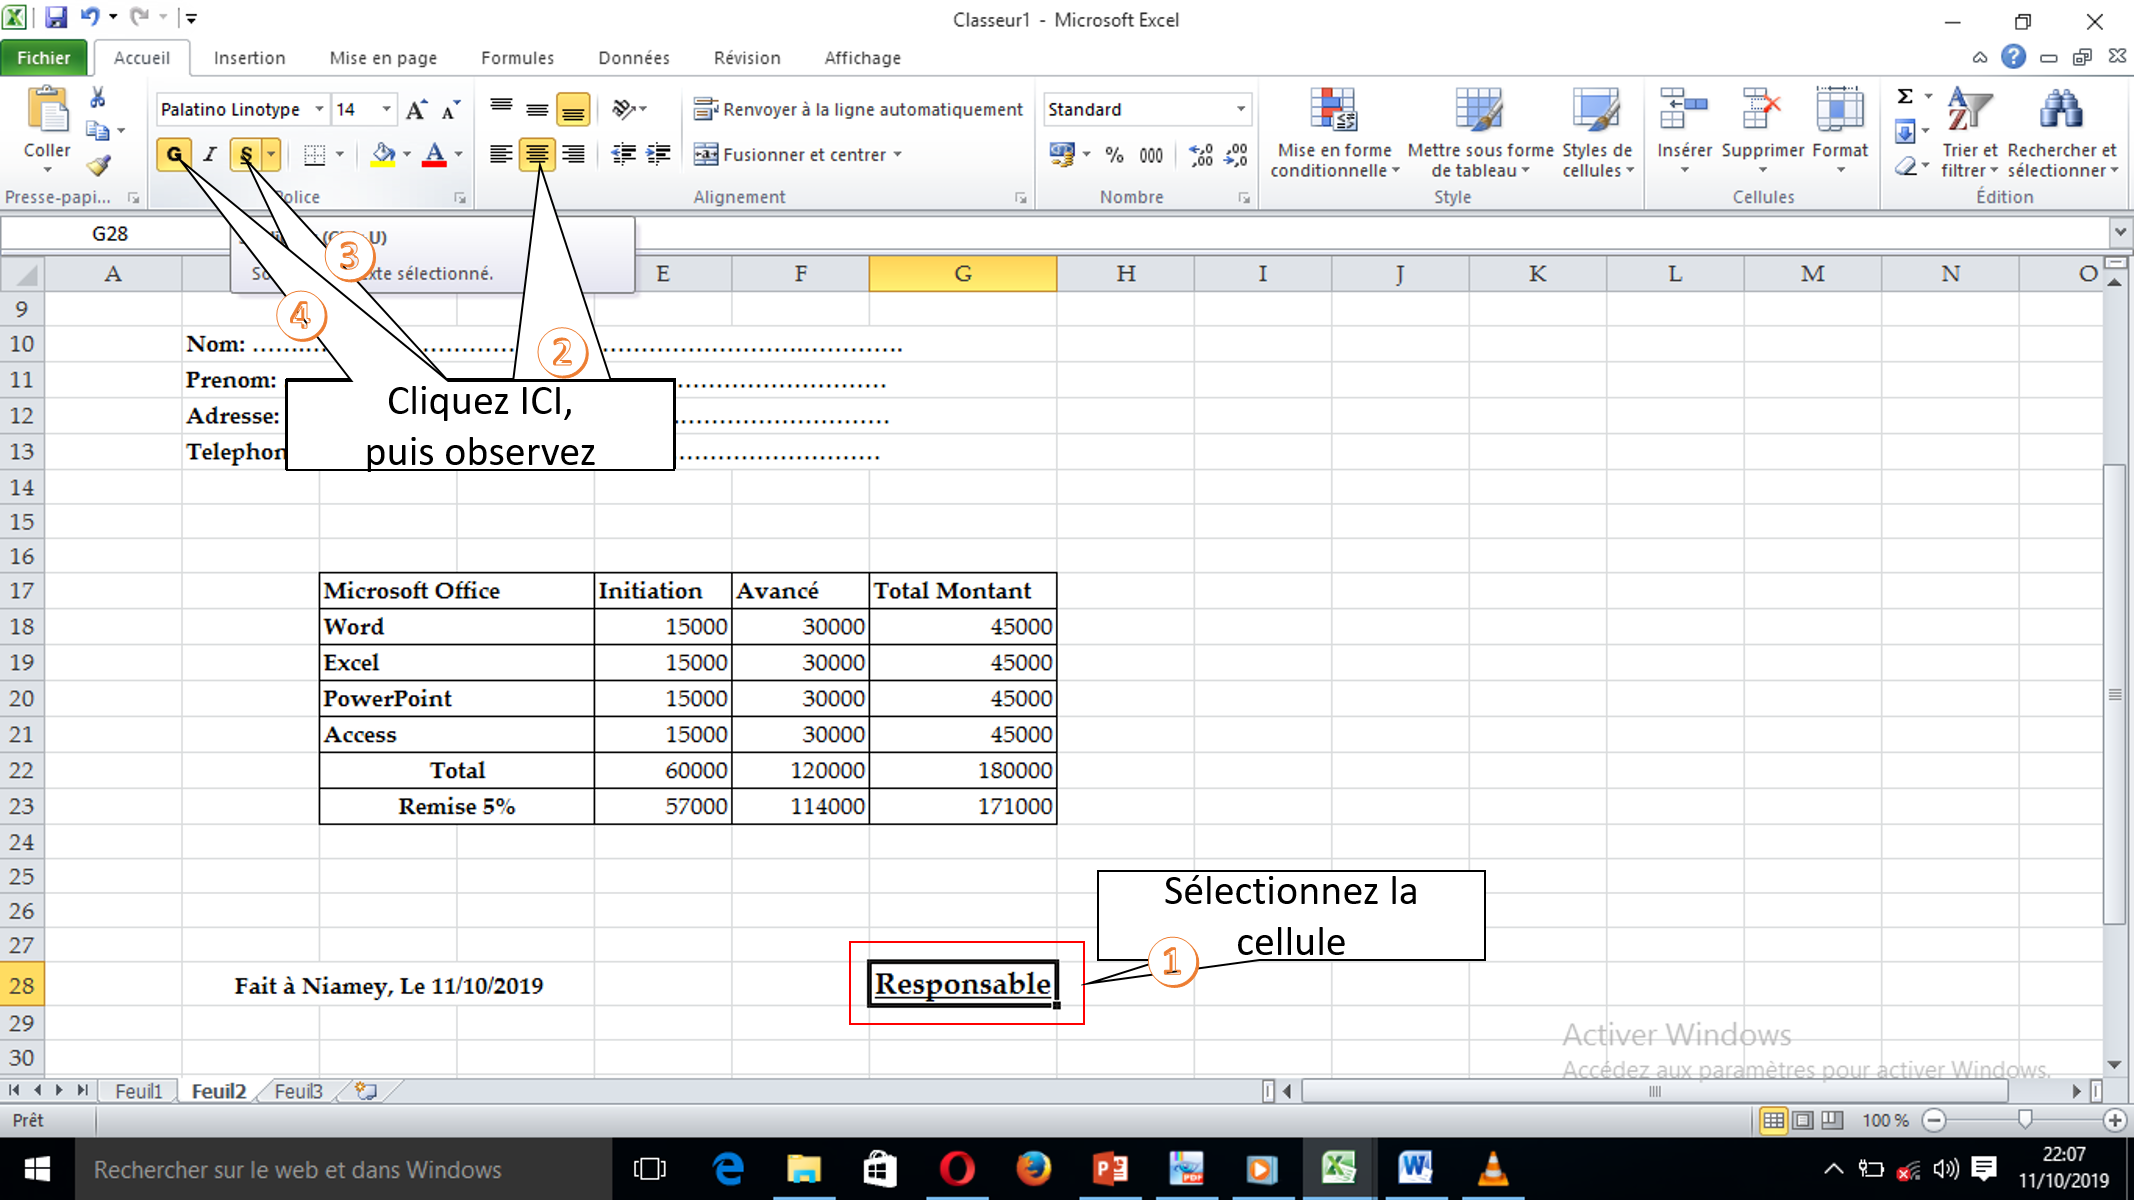
\includegraphics[ width=\linewidth,height=0.705\paperheight]{img/31}
\end{landscape}
\begin{landscape} 		
	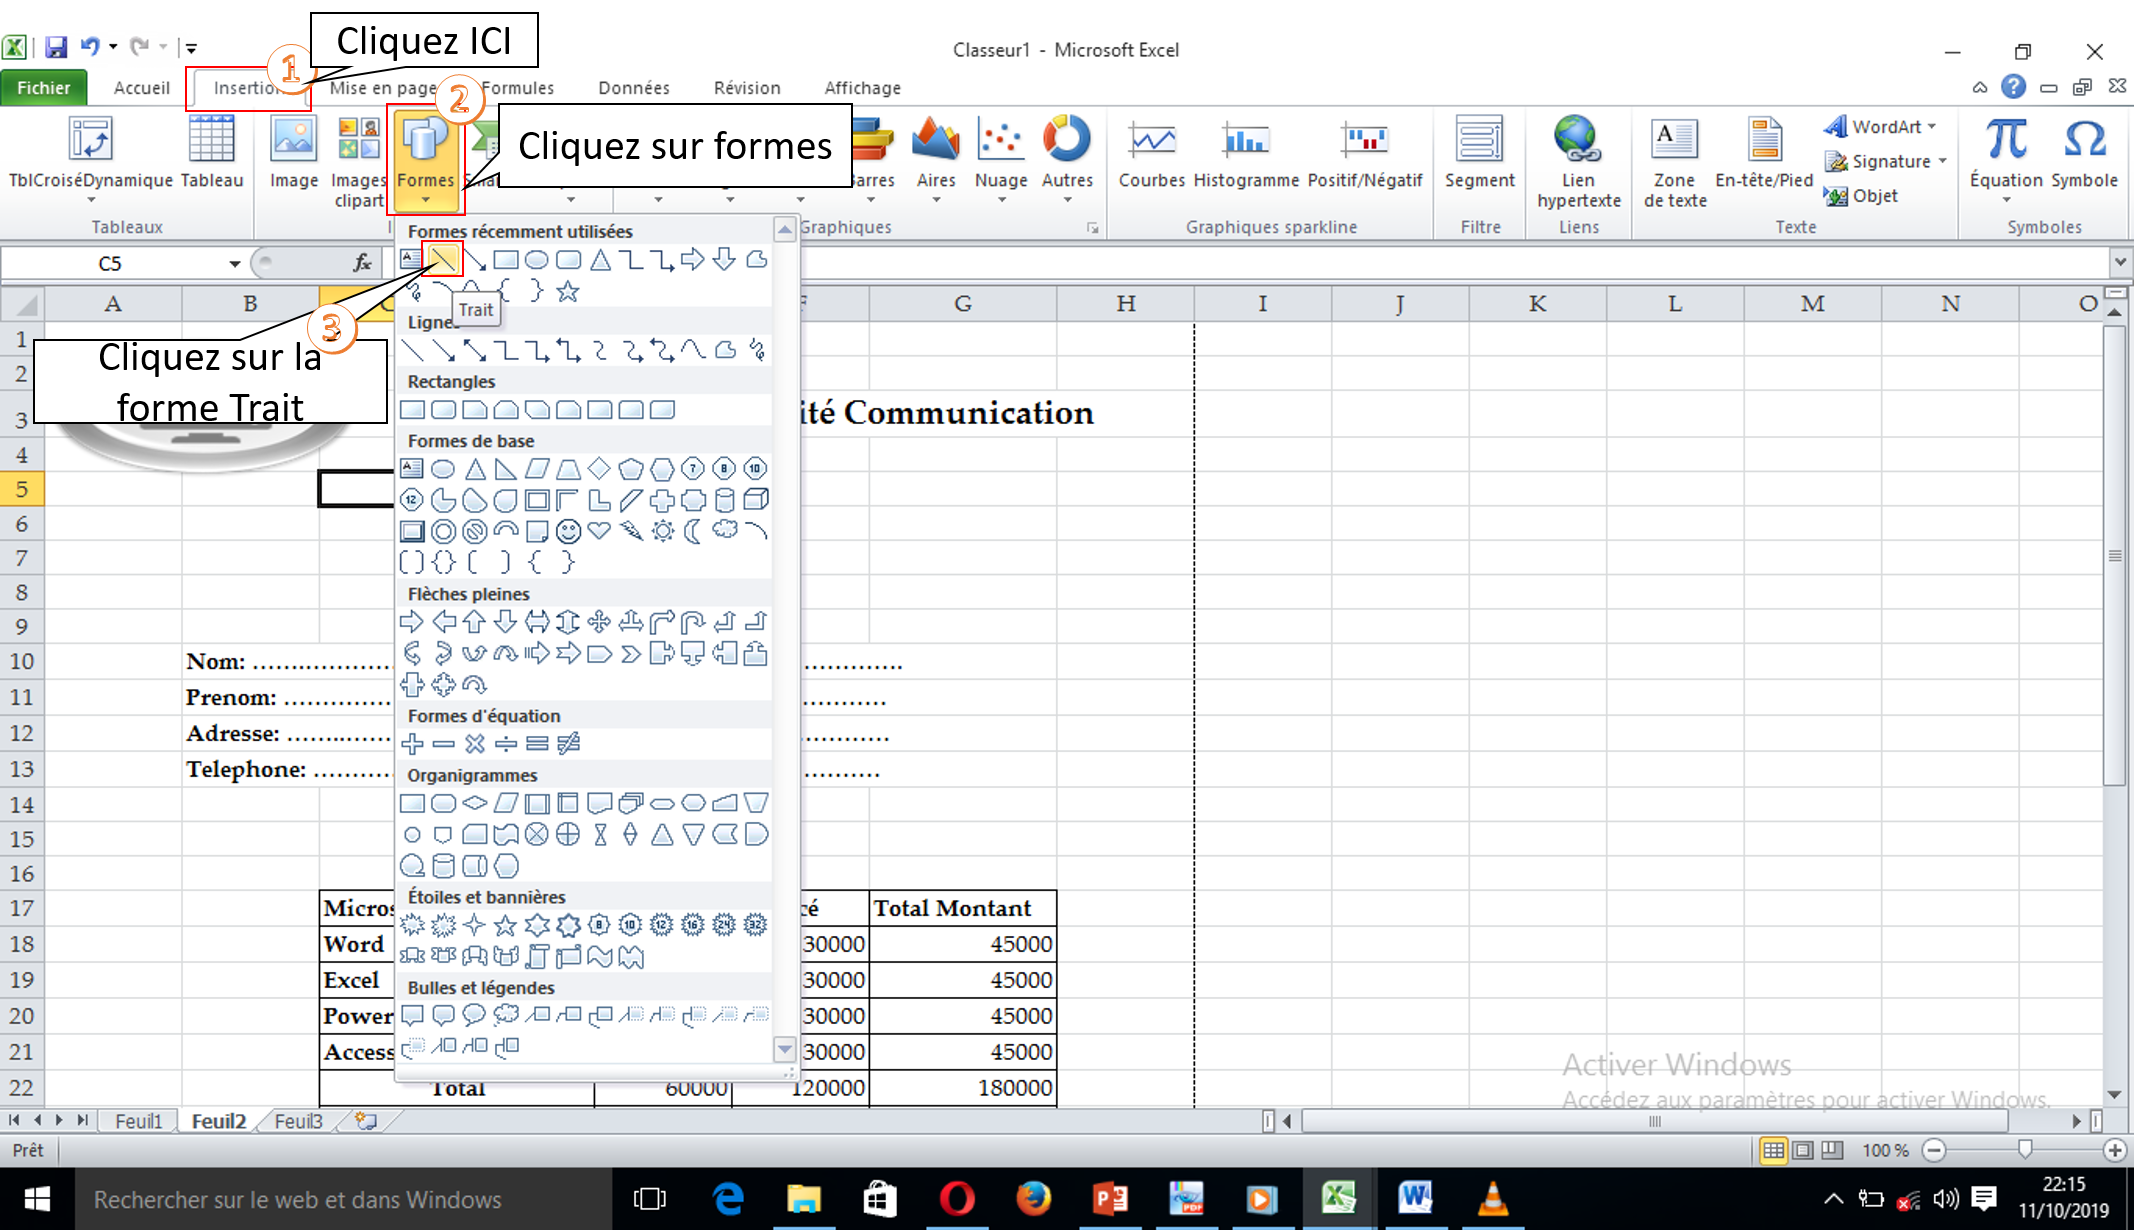
\includegraphics[ width=\linewidth,height=0.705\paperheight]{img/32}
\end{landscape}
\begin{landscape} 		
	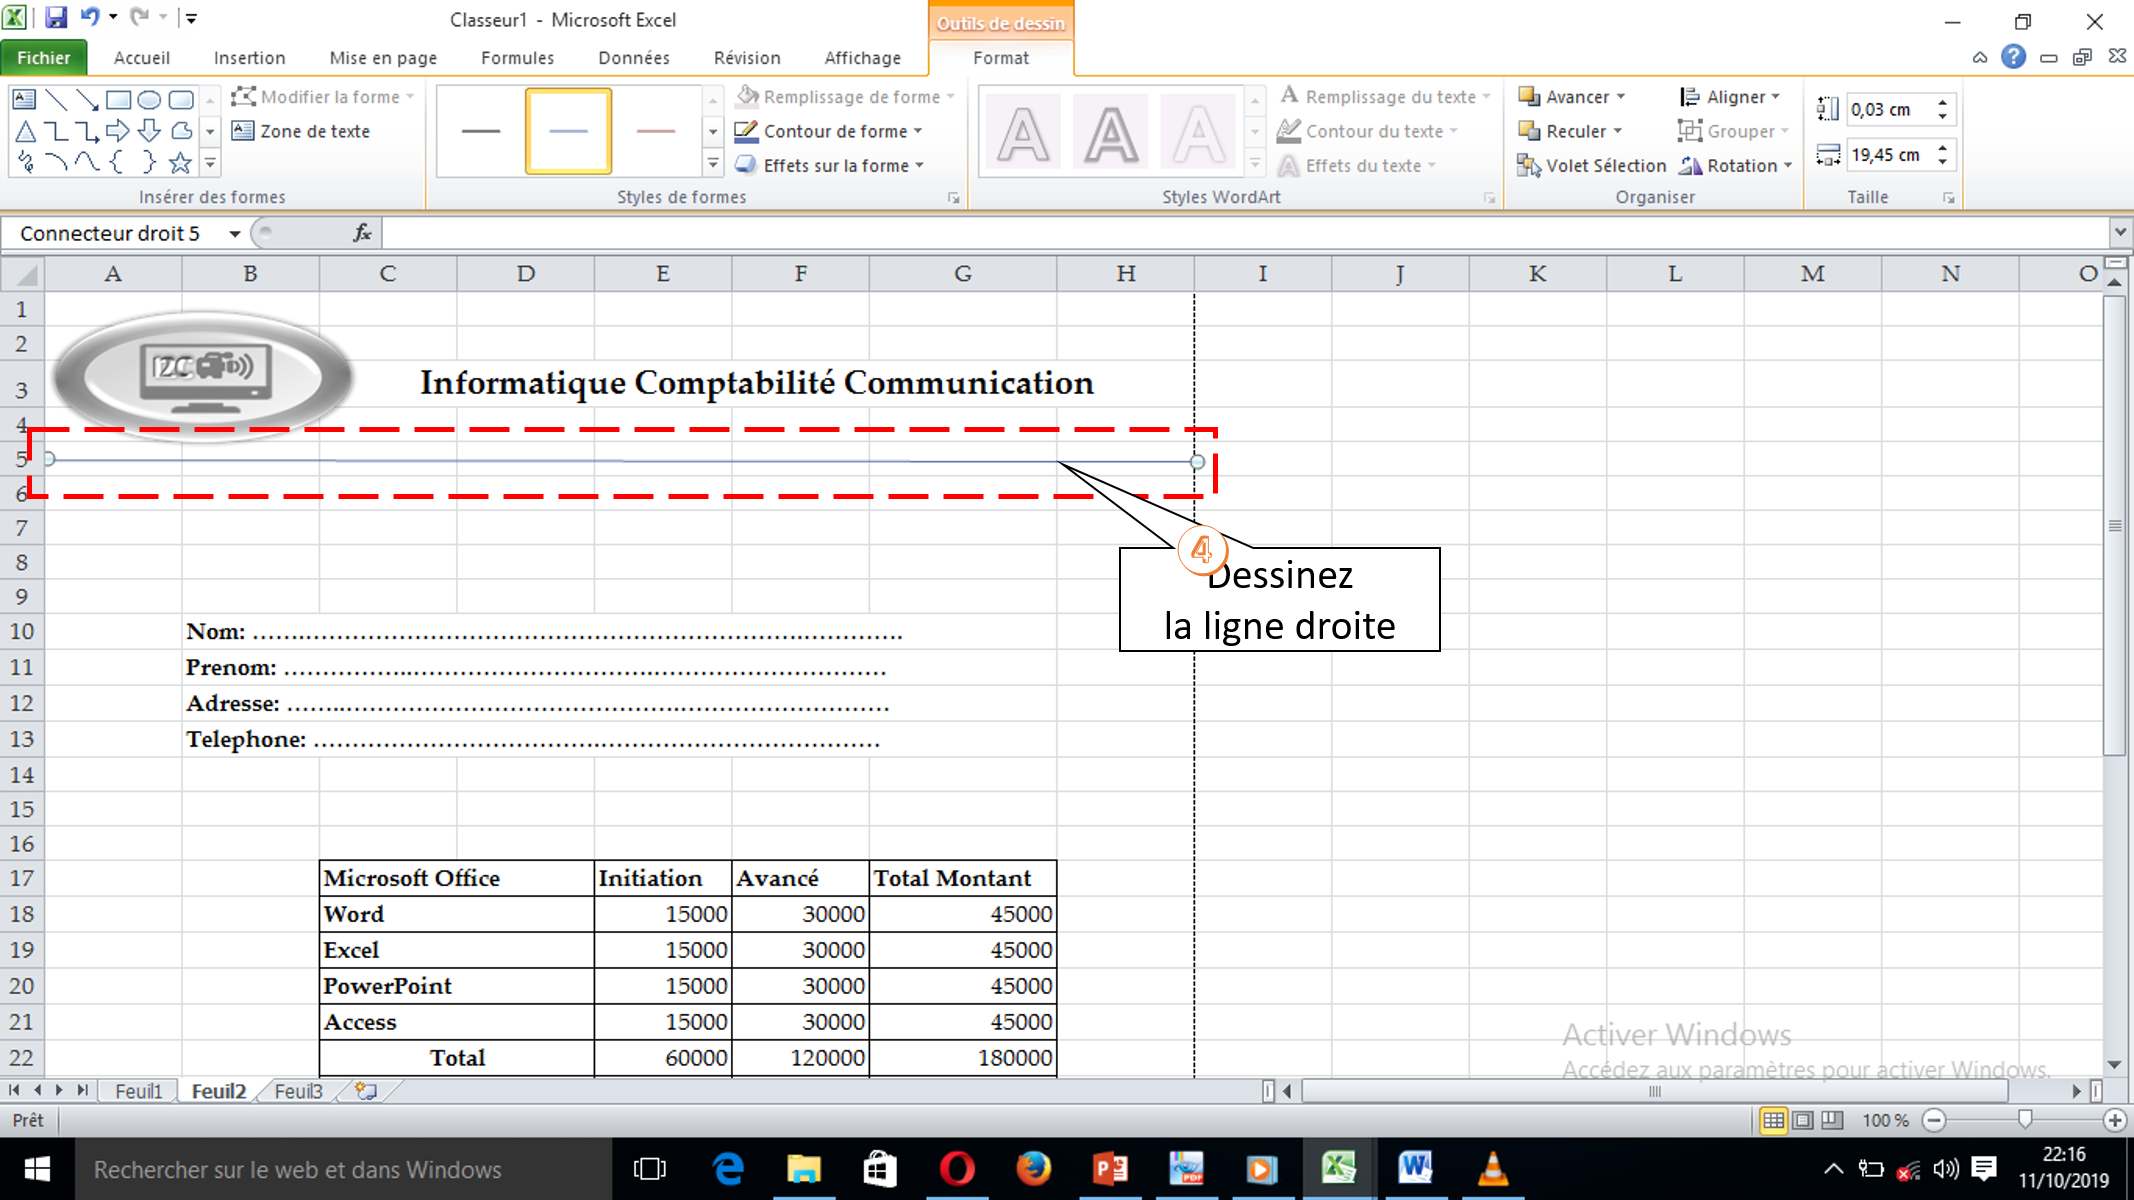
\includegraphics[ width=\linewidth,height=0.705\paperheight]{img/33}
\end{landscape}
\begin{landscape} 		
	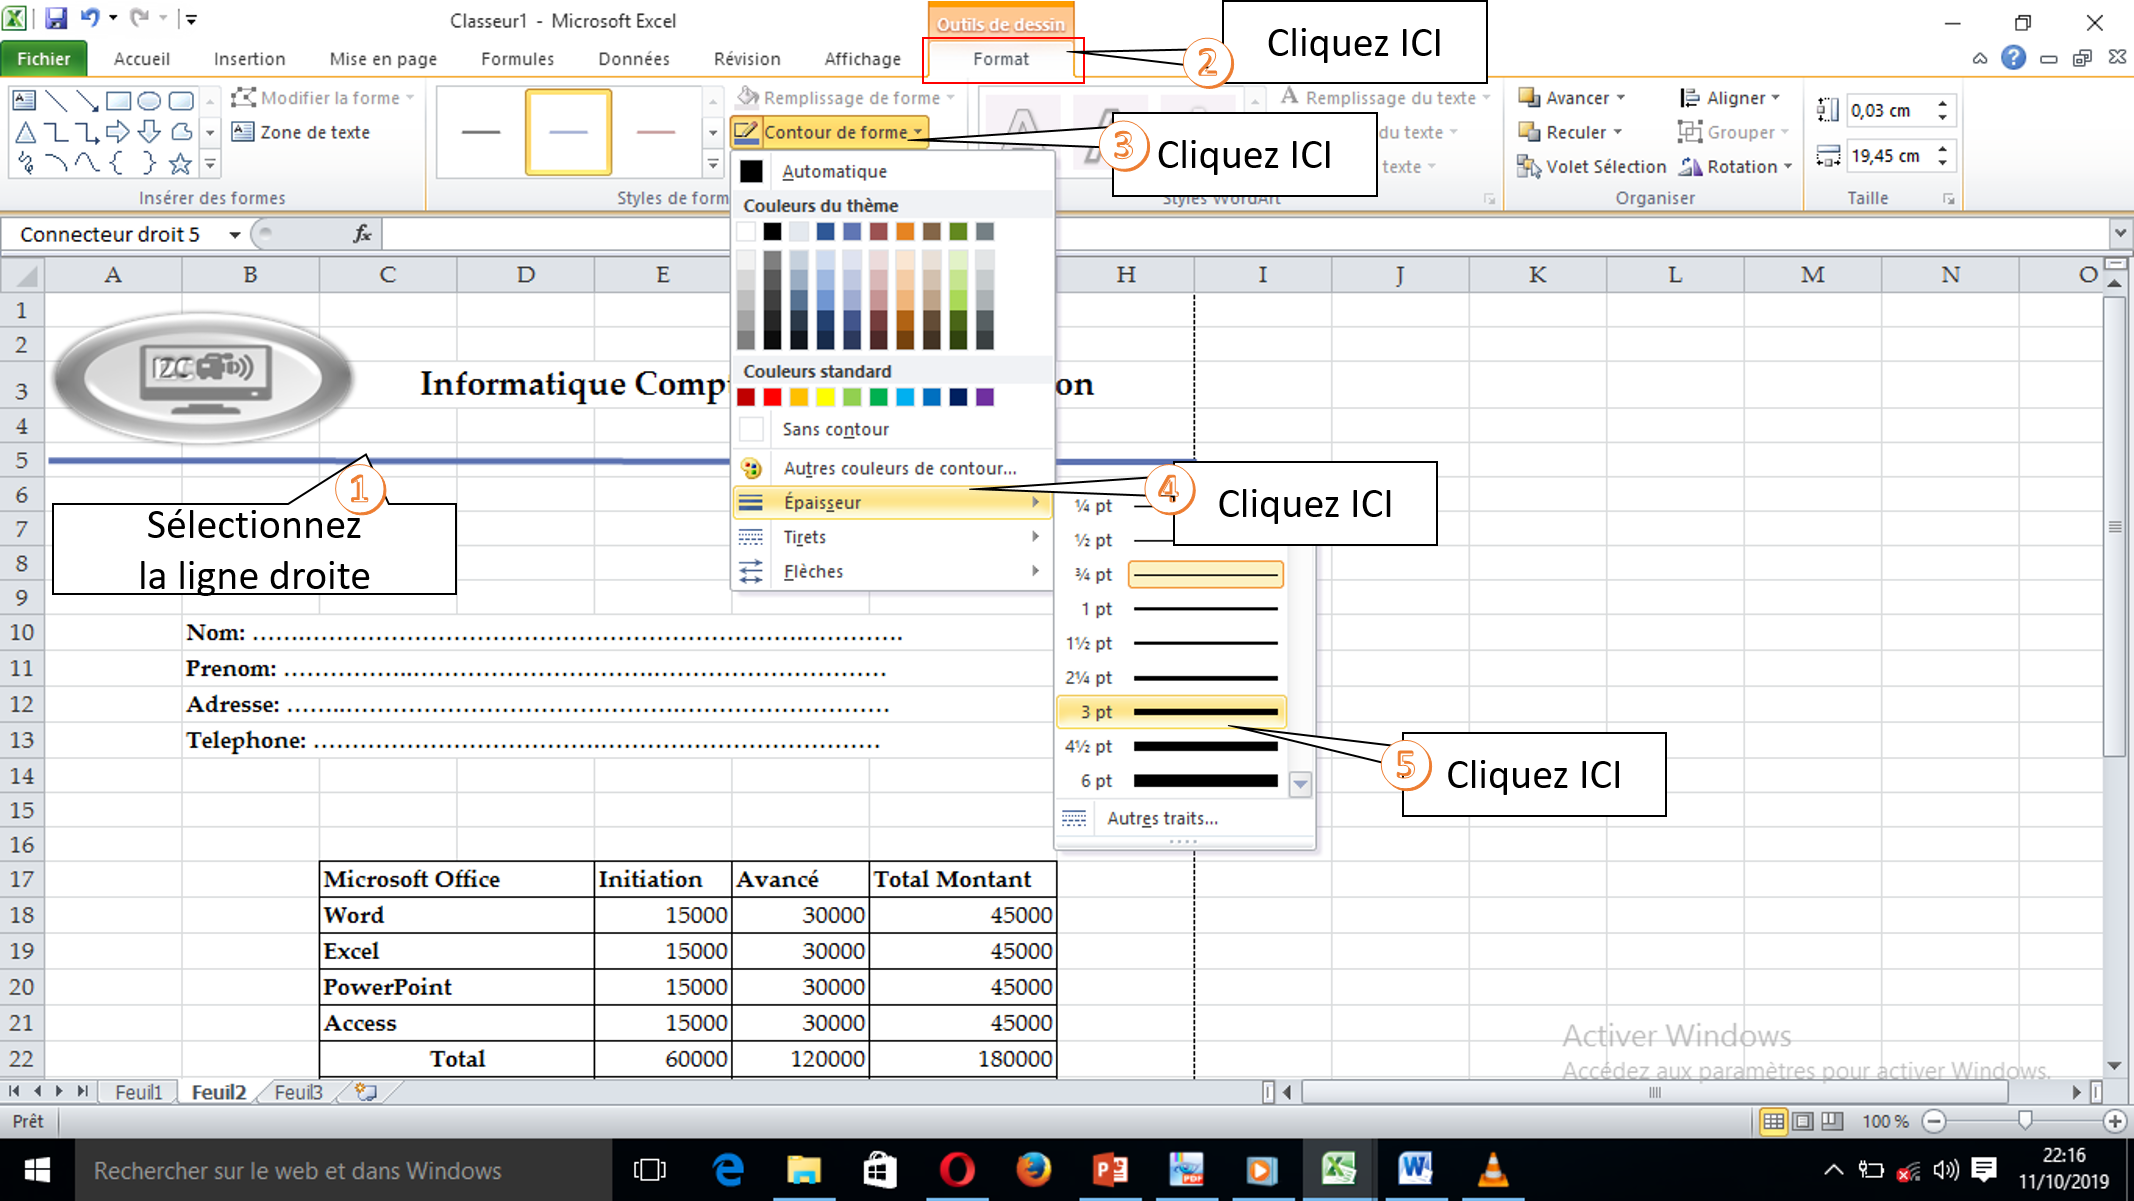
\includegraphics[ width=\linewidth,height=0.705\paperheight]{img/34}
\end{landscape}
\begin{landscape} 		
	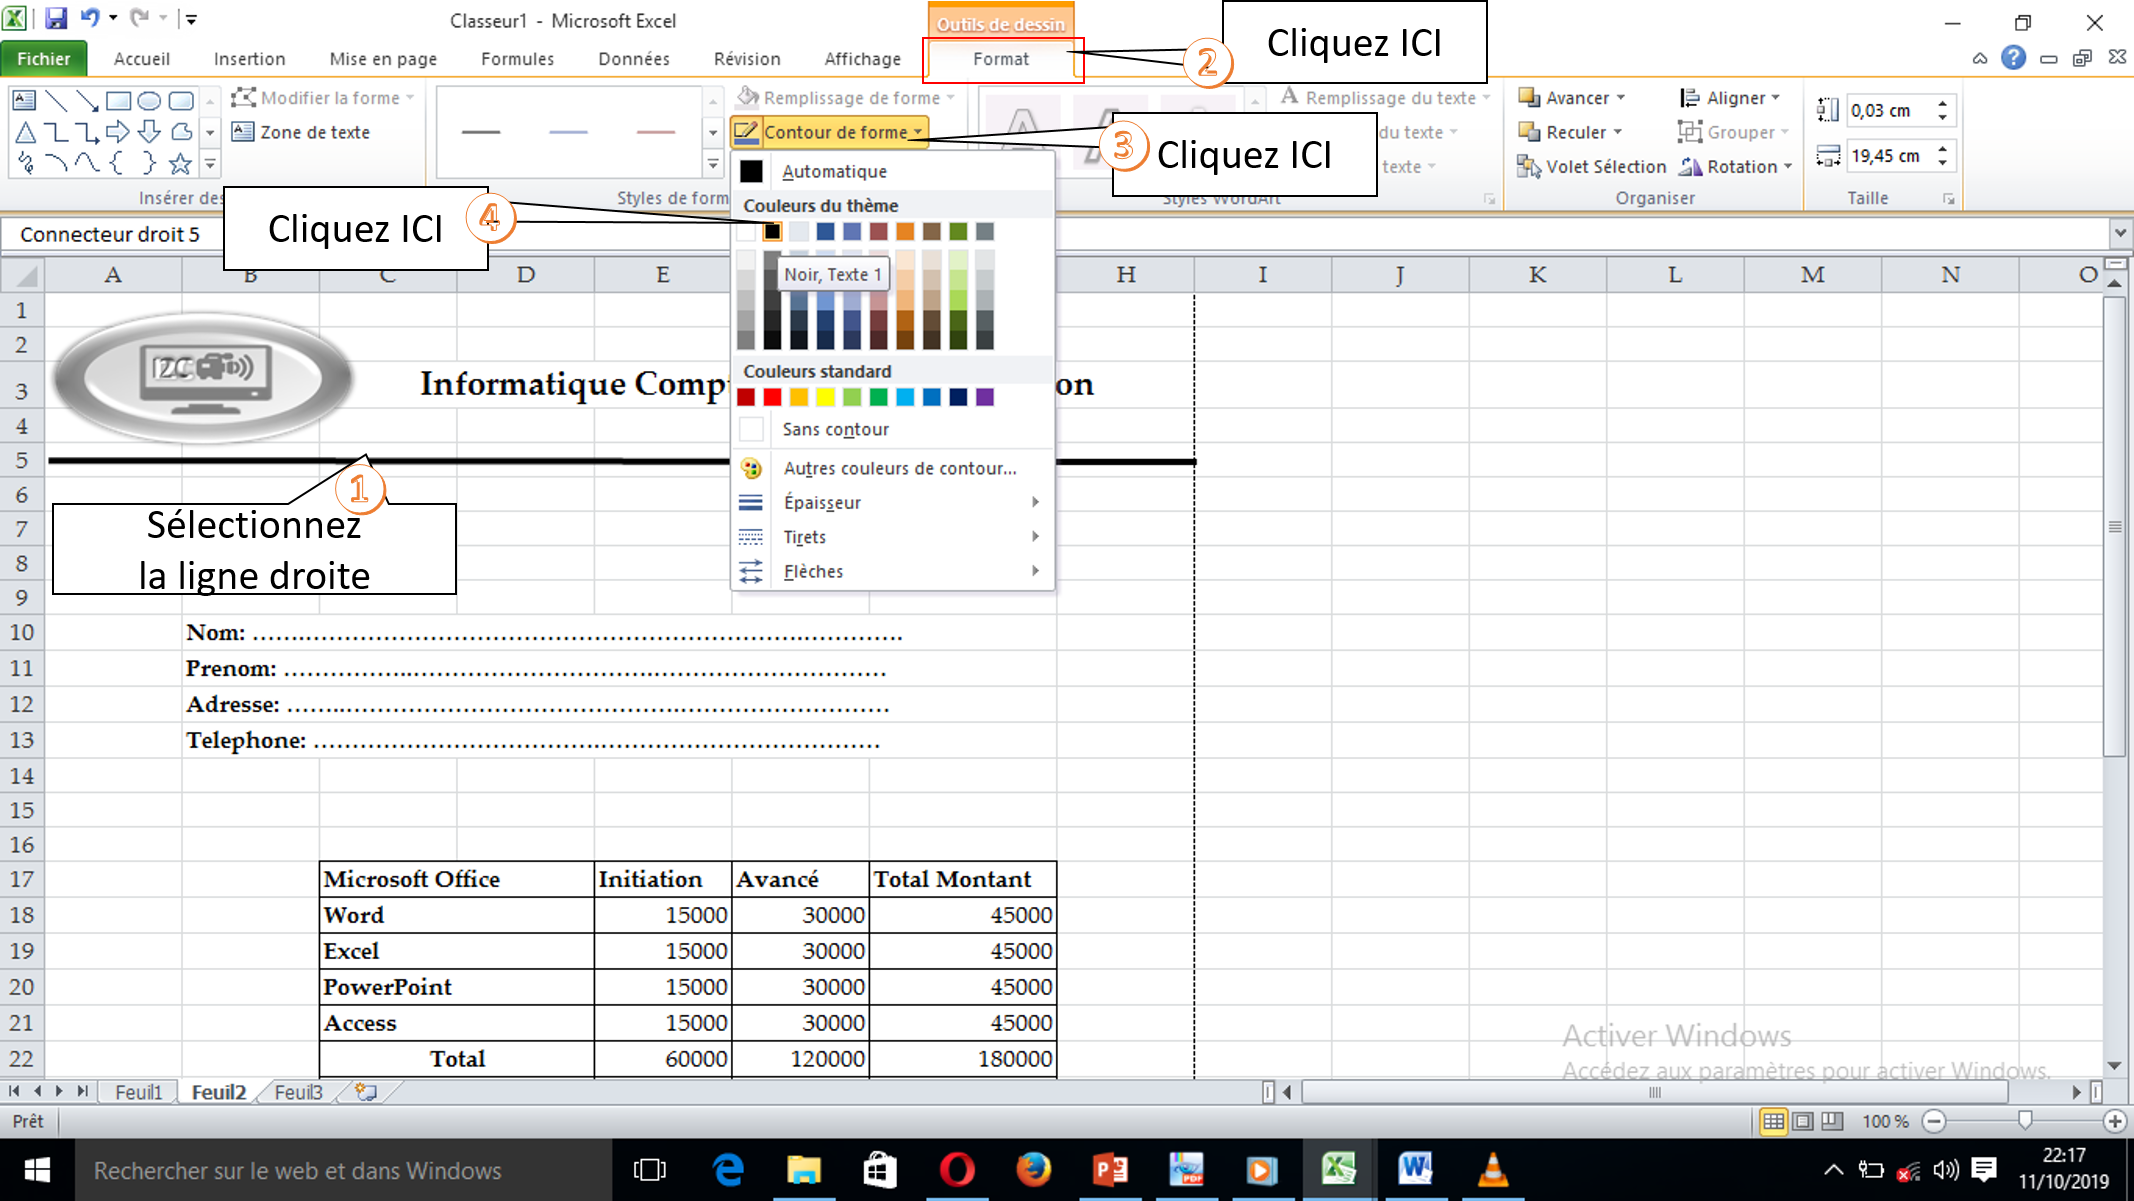
\includegraphics[ width=\linewidth,height=0.705\paperheight]{img/35}
\end{landscape}
\begin{landscape} 		
	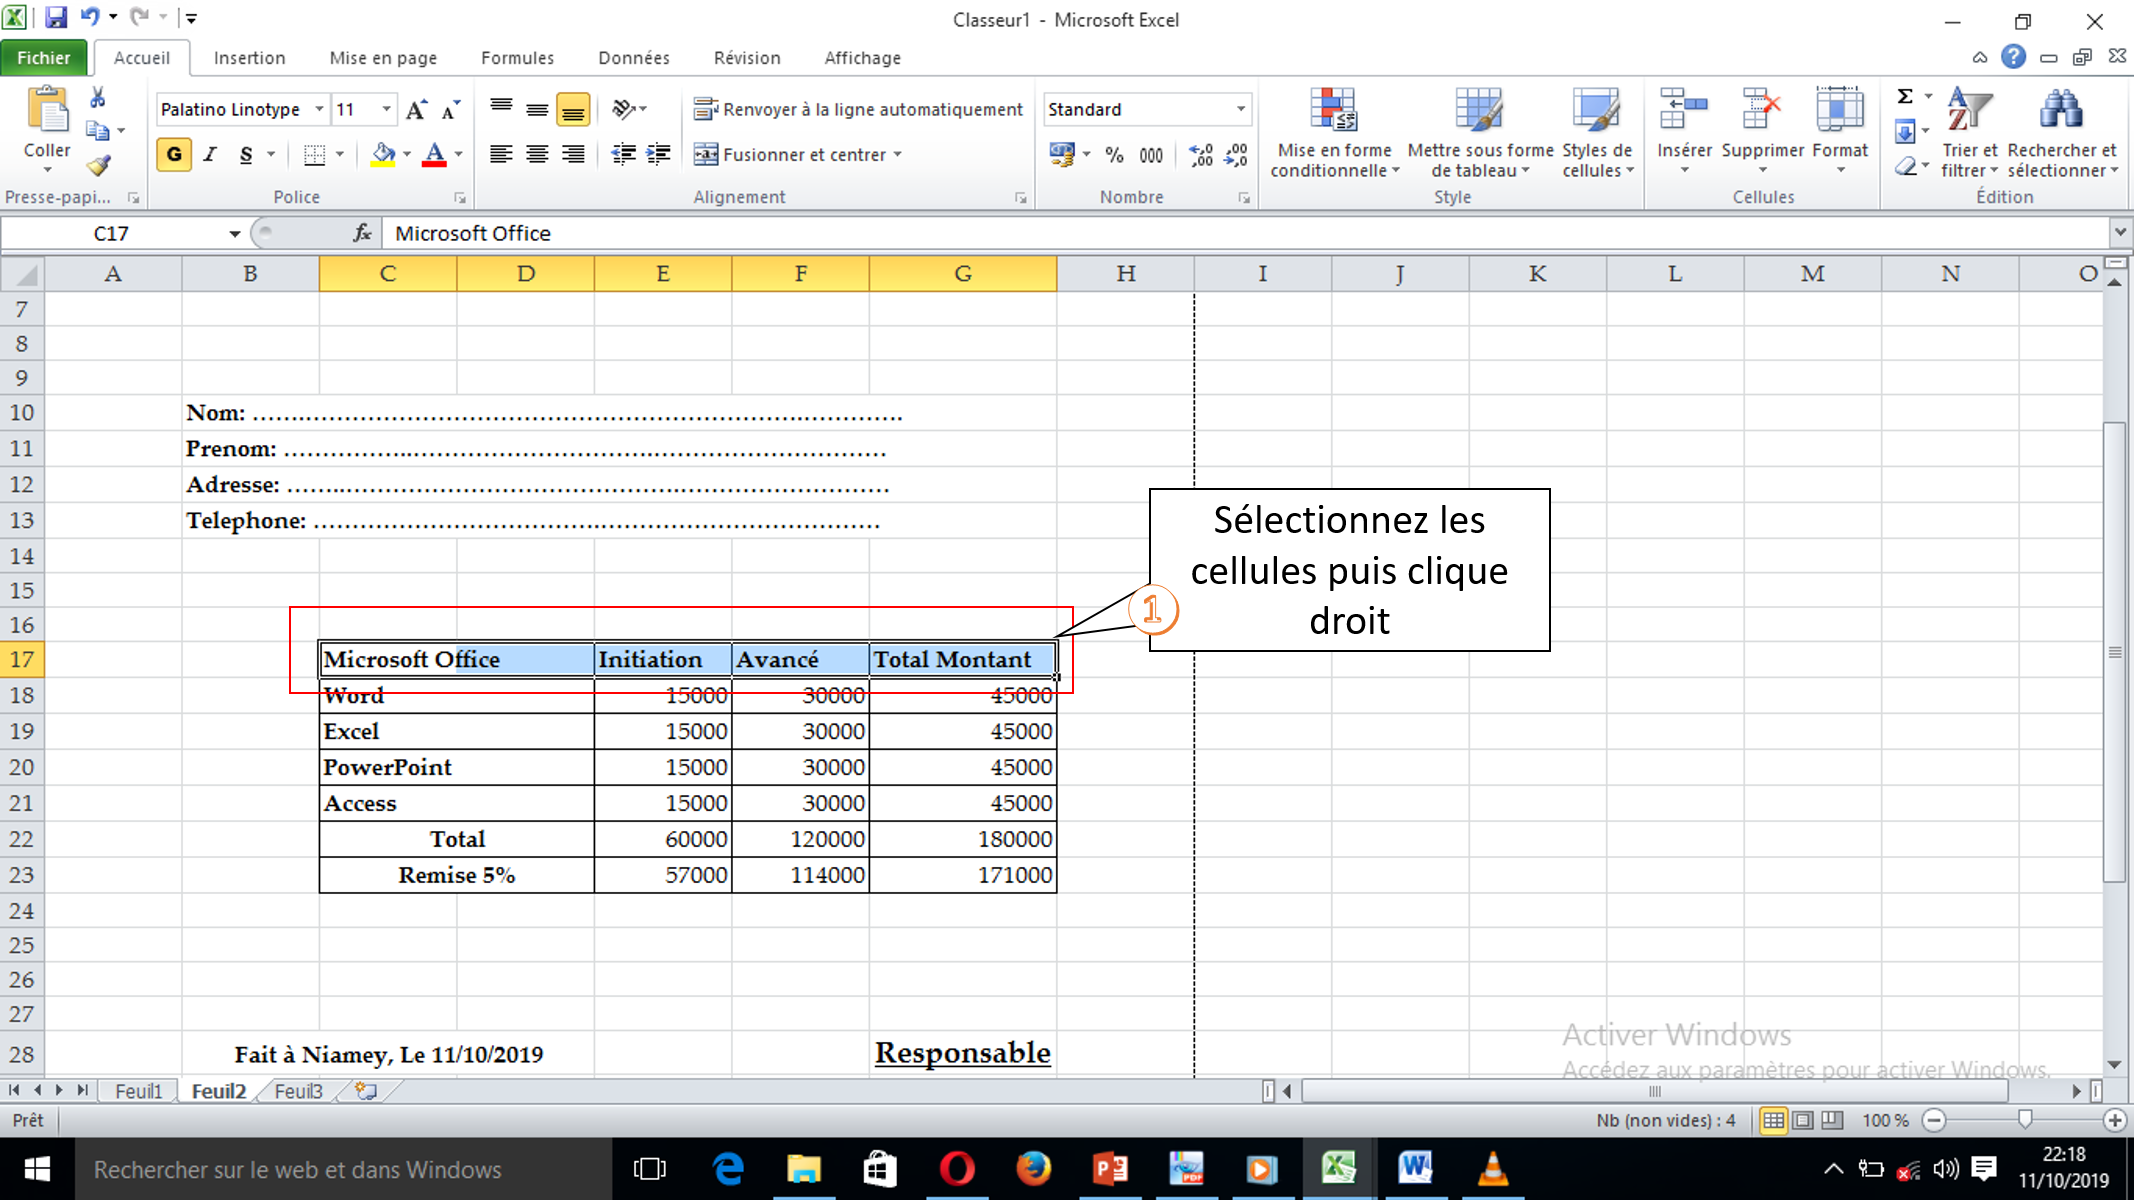
\includegraphics[ width=\linewidth,height=0.705\paperheight]{img/36}
\end{landscape}
\begin{landscape} 		
	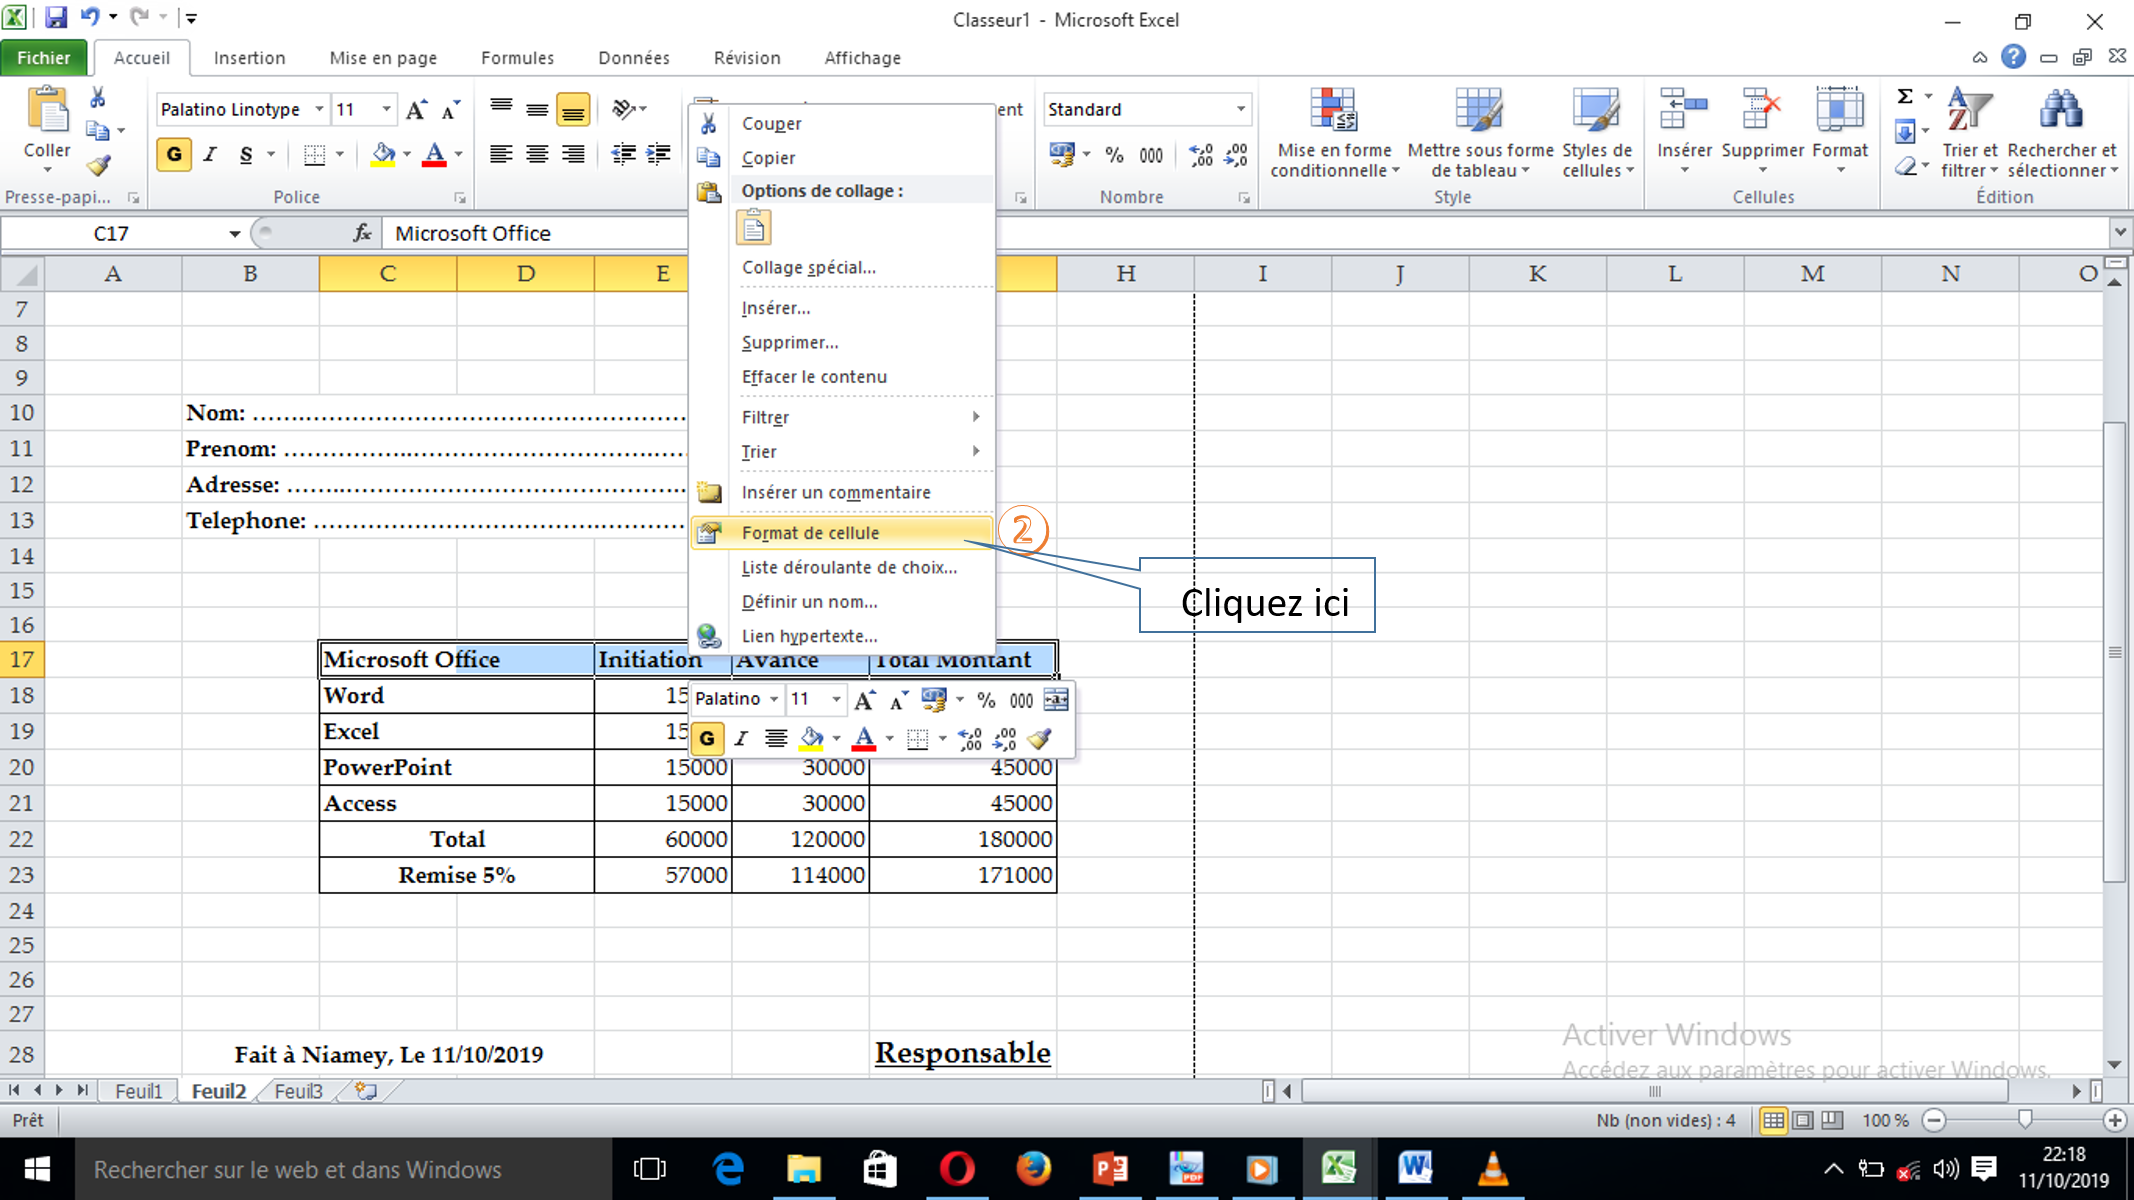
\includegraphics[ width=\linewidth,height=0.705\paperheight]{img/37}
\end{landscape}
\begin{landscape} 		
	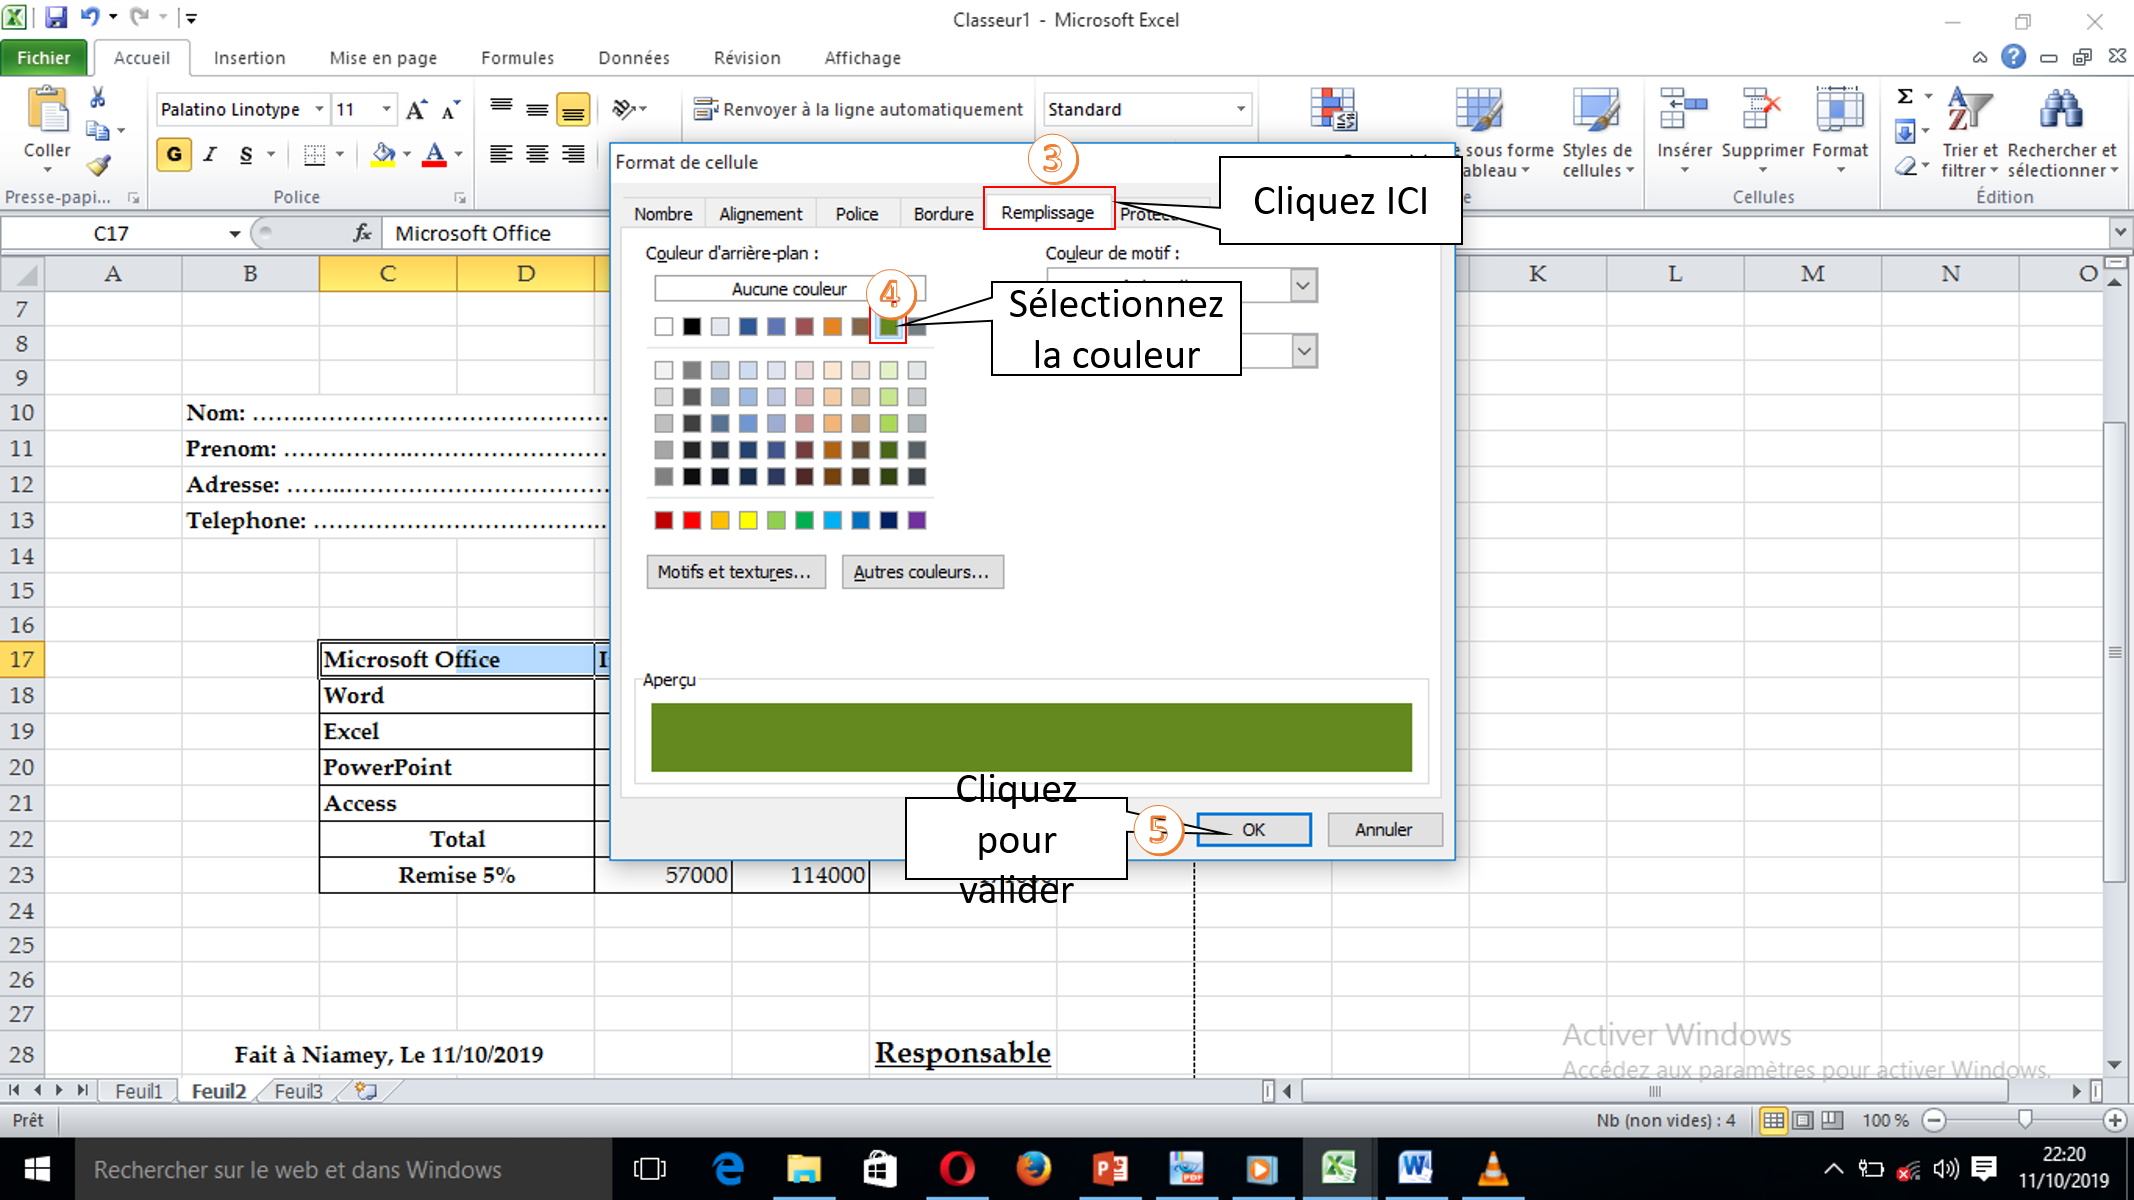
\includegraphics[ width=\linewidth,height=0.705\paperheight]{img/38}
\end{landscape}
\begin{landscape} 		
	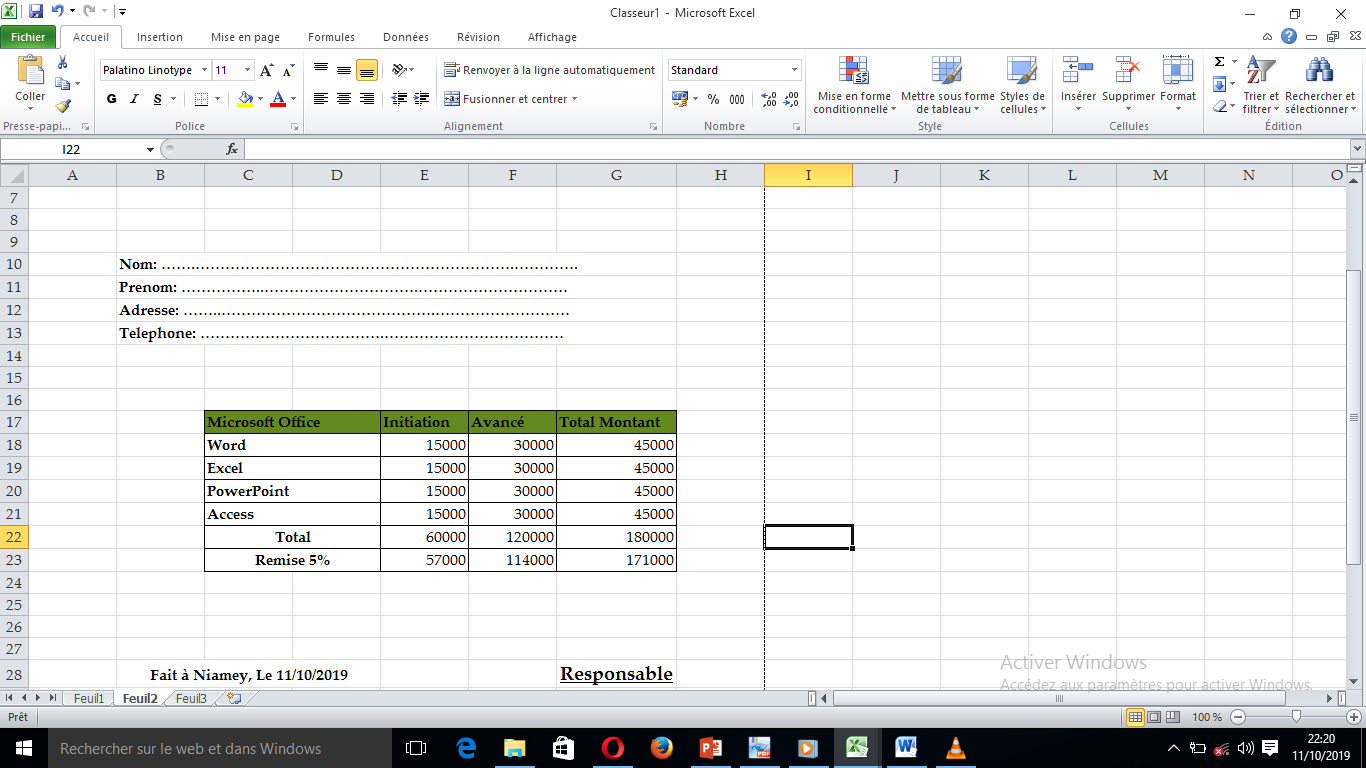
\includegraphics[ width=\linewidth,height=0.705\paperheight]{img/39}
\end{landscape}
\begin{landscape} 		
	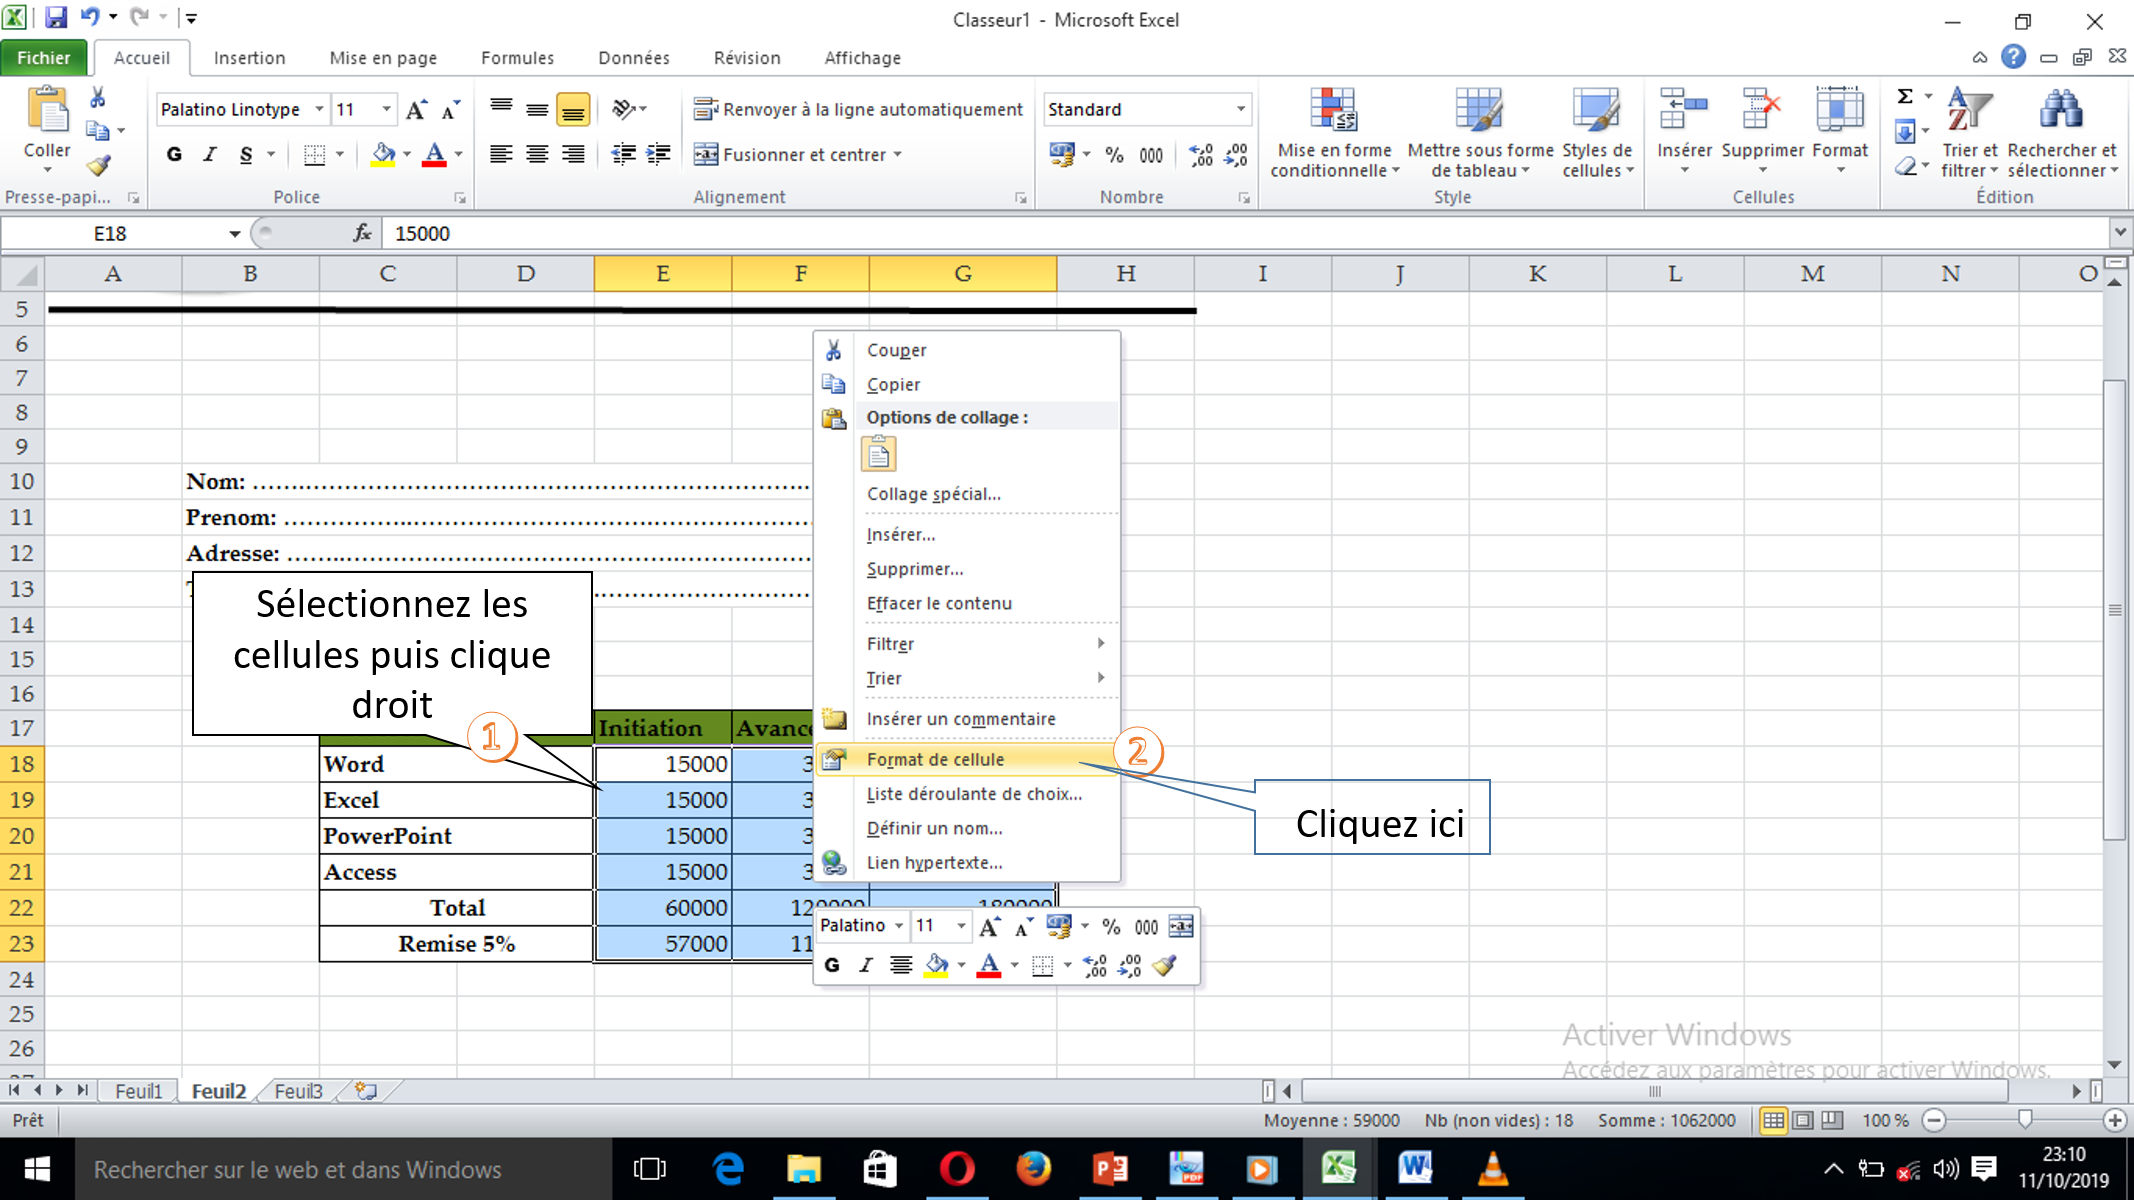
\includegraphics[ width=\linewidth,height=0.705\paperheight]{img/40}
\end{landscape}
\begin{landscape} 		
	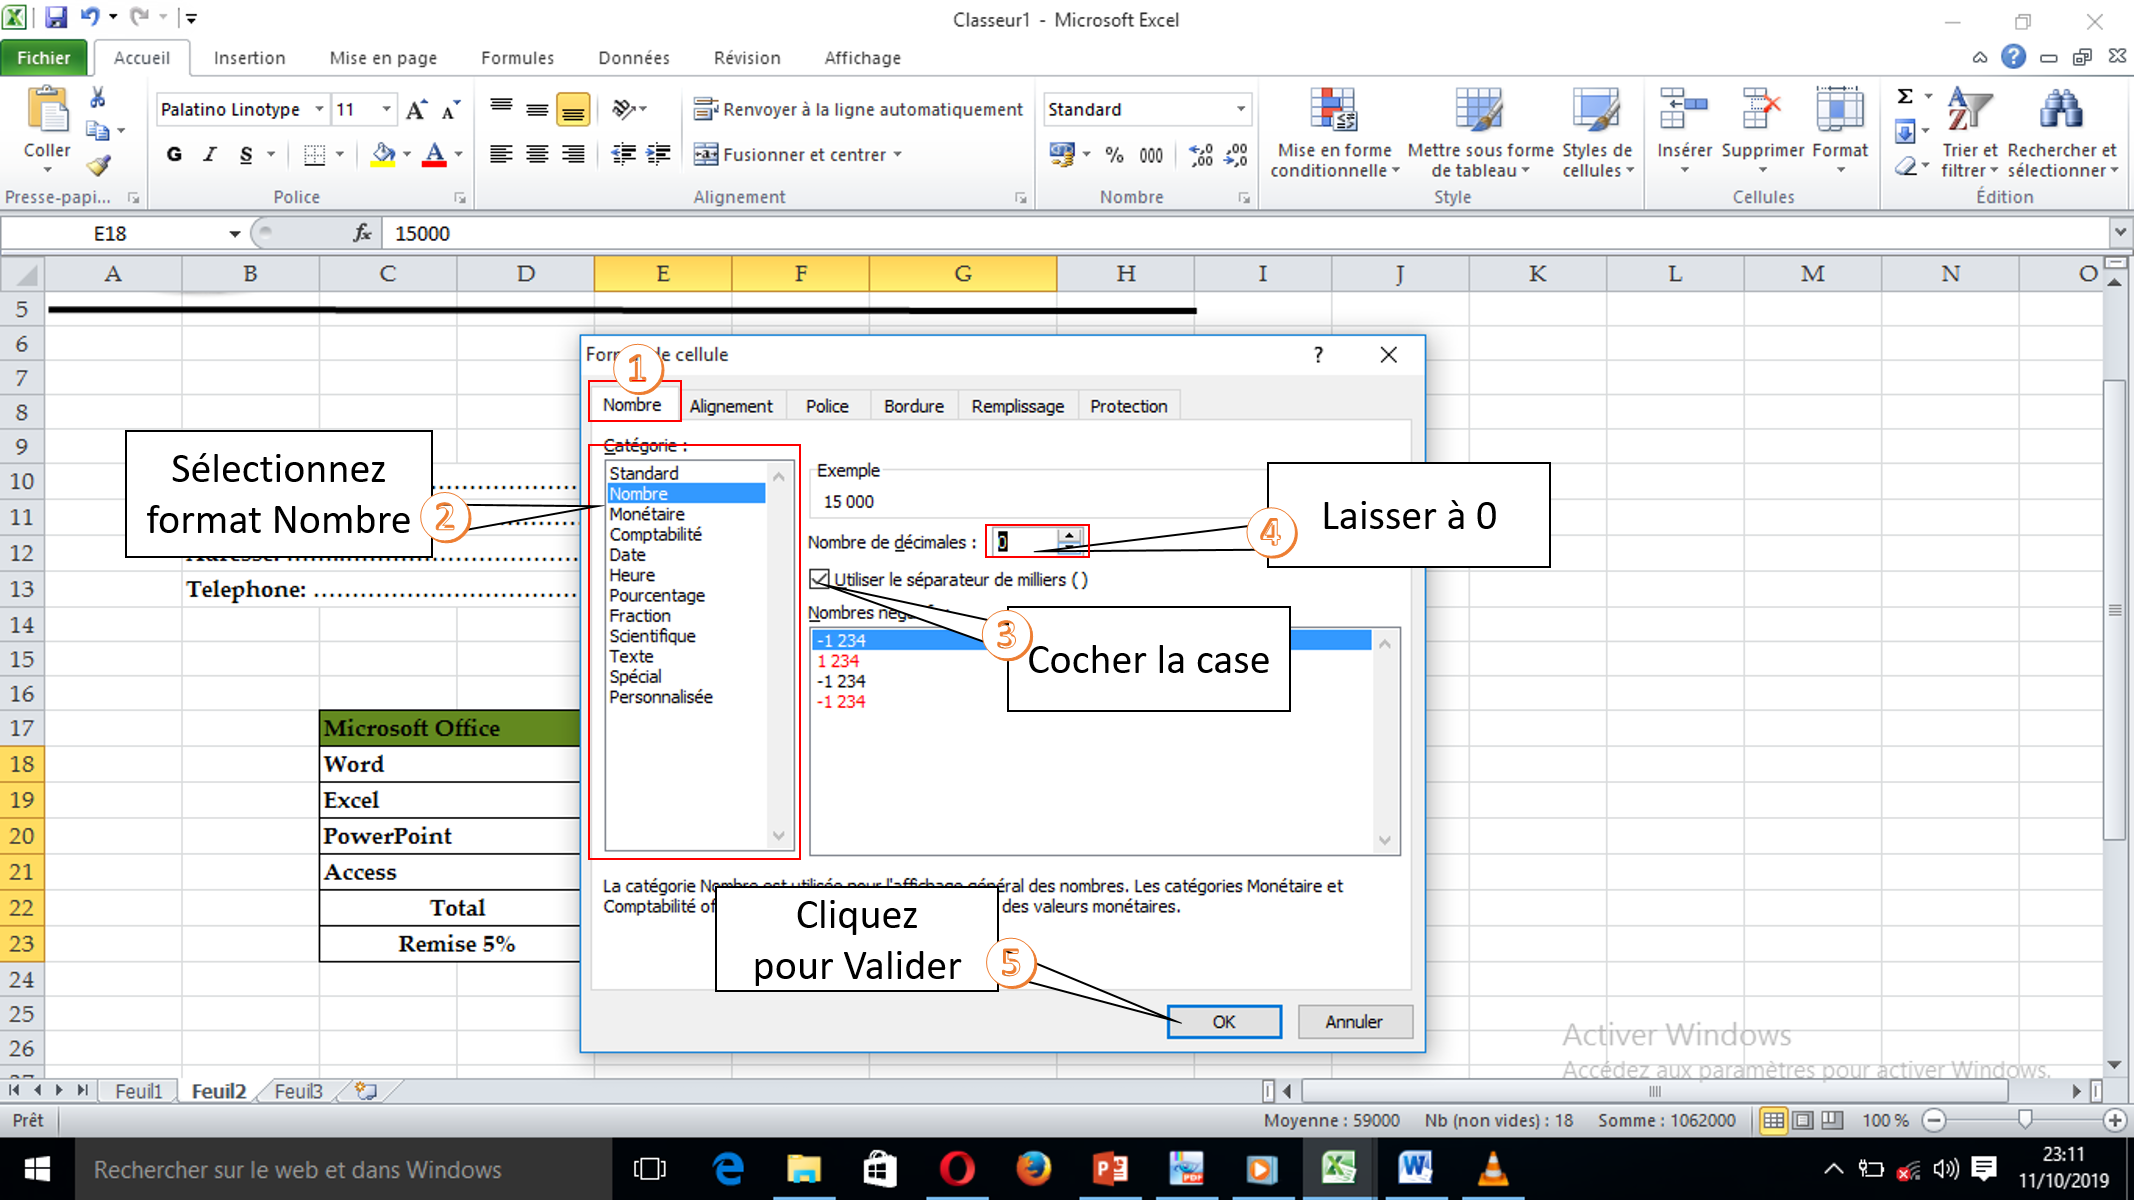
\includegraphics[ width=\linewidth,height=0.705\paperheight]{img/41}
\end{landscape}
\begin{landscape} 		
	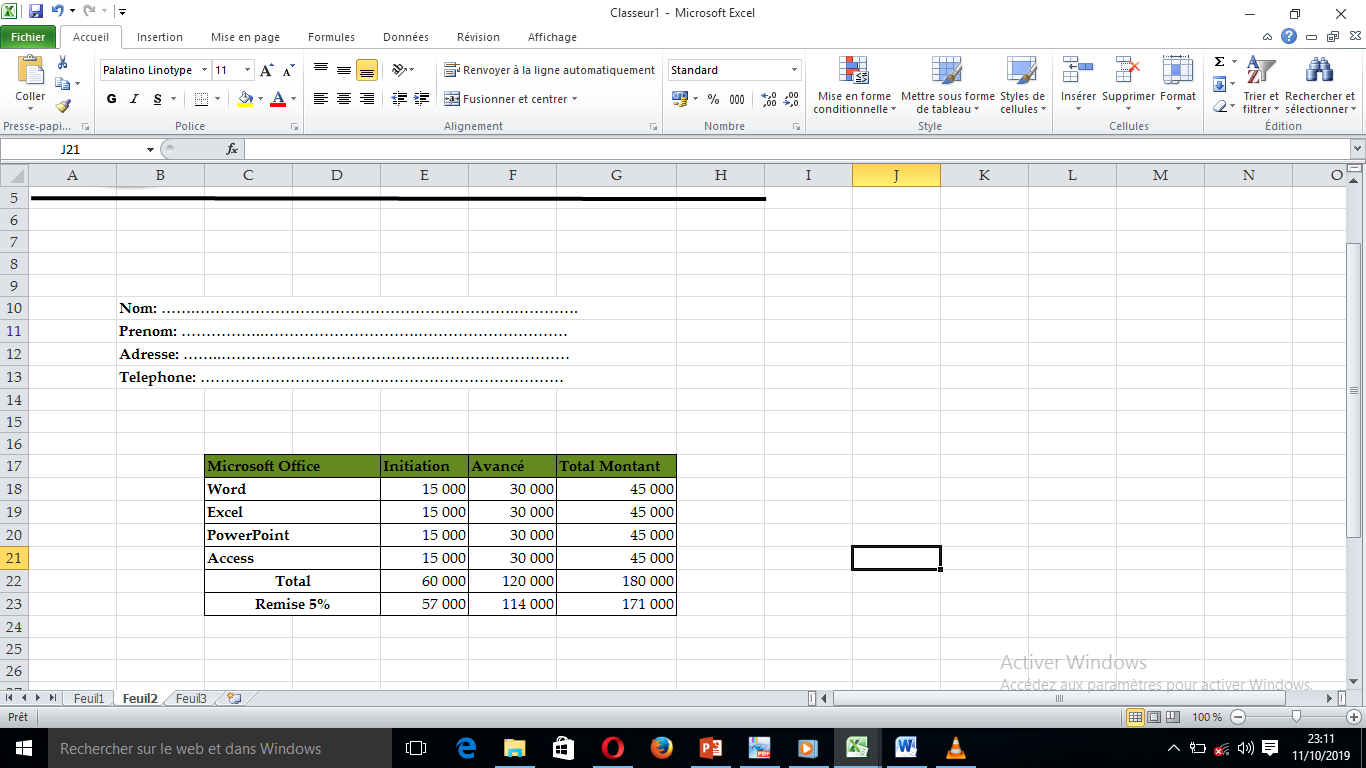
\includegraphics[ width=\linewidth,height=0.705\paperheight]{img/42}
\end{landscape}
\begin{landscape} 		
	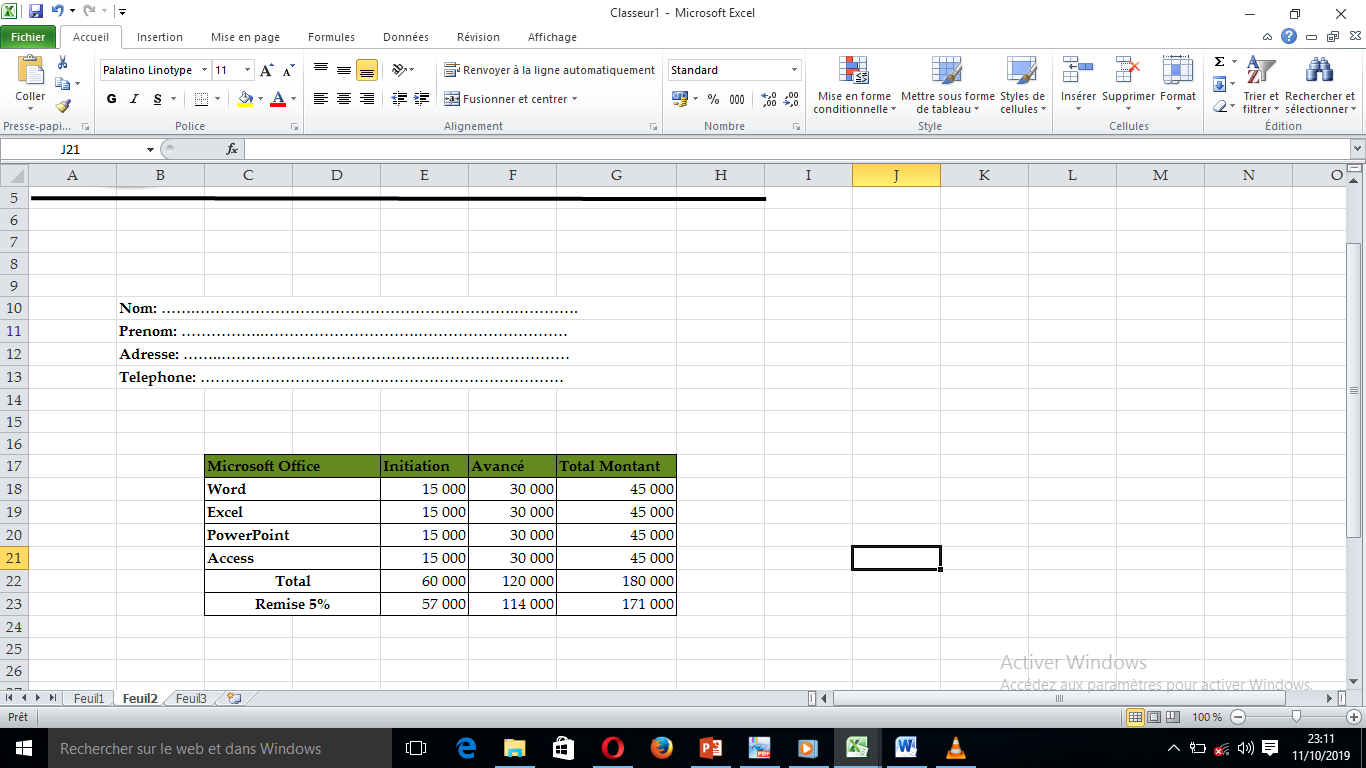
\includegraphics[ width=\linewidth,height=0.705\paperheight]{img/43}
\end{landscape}
\begin{landscape} 		
	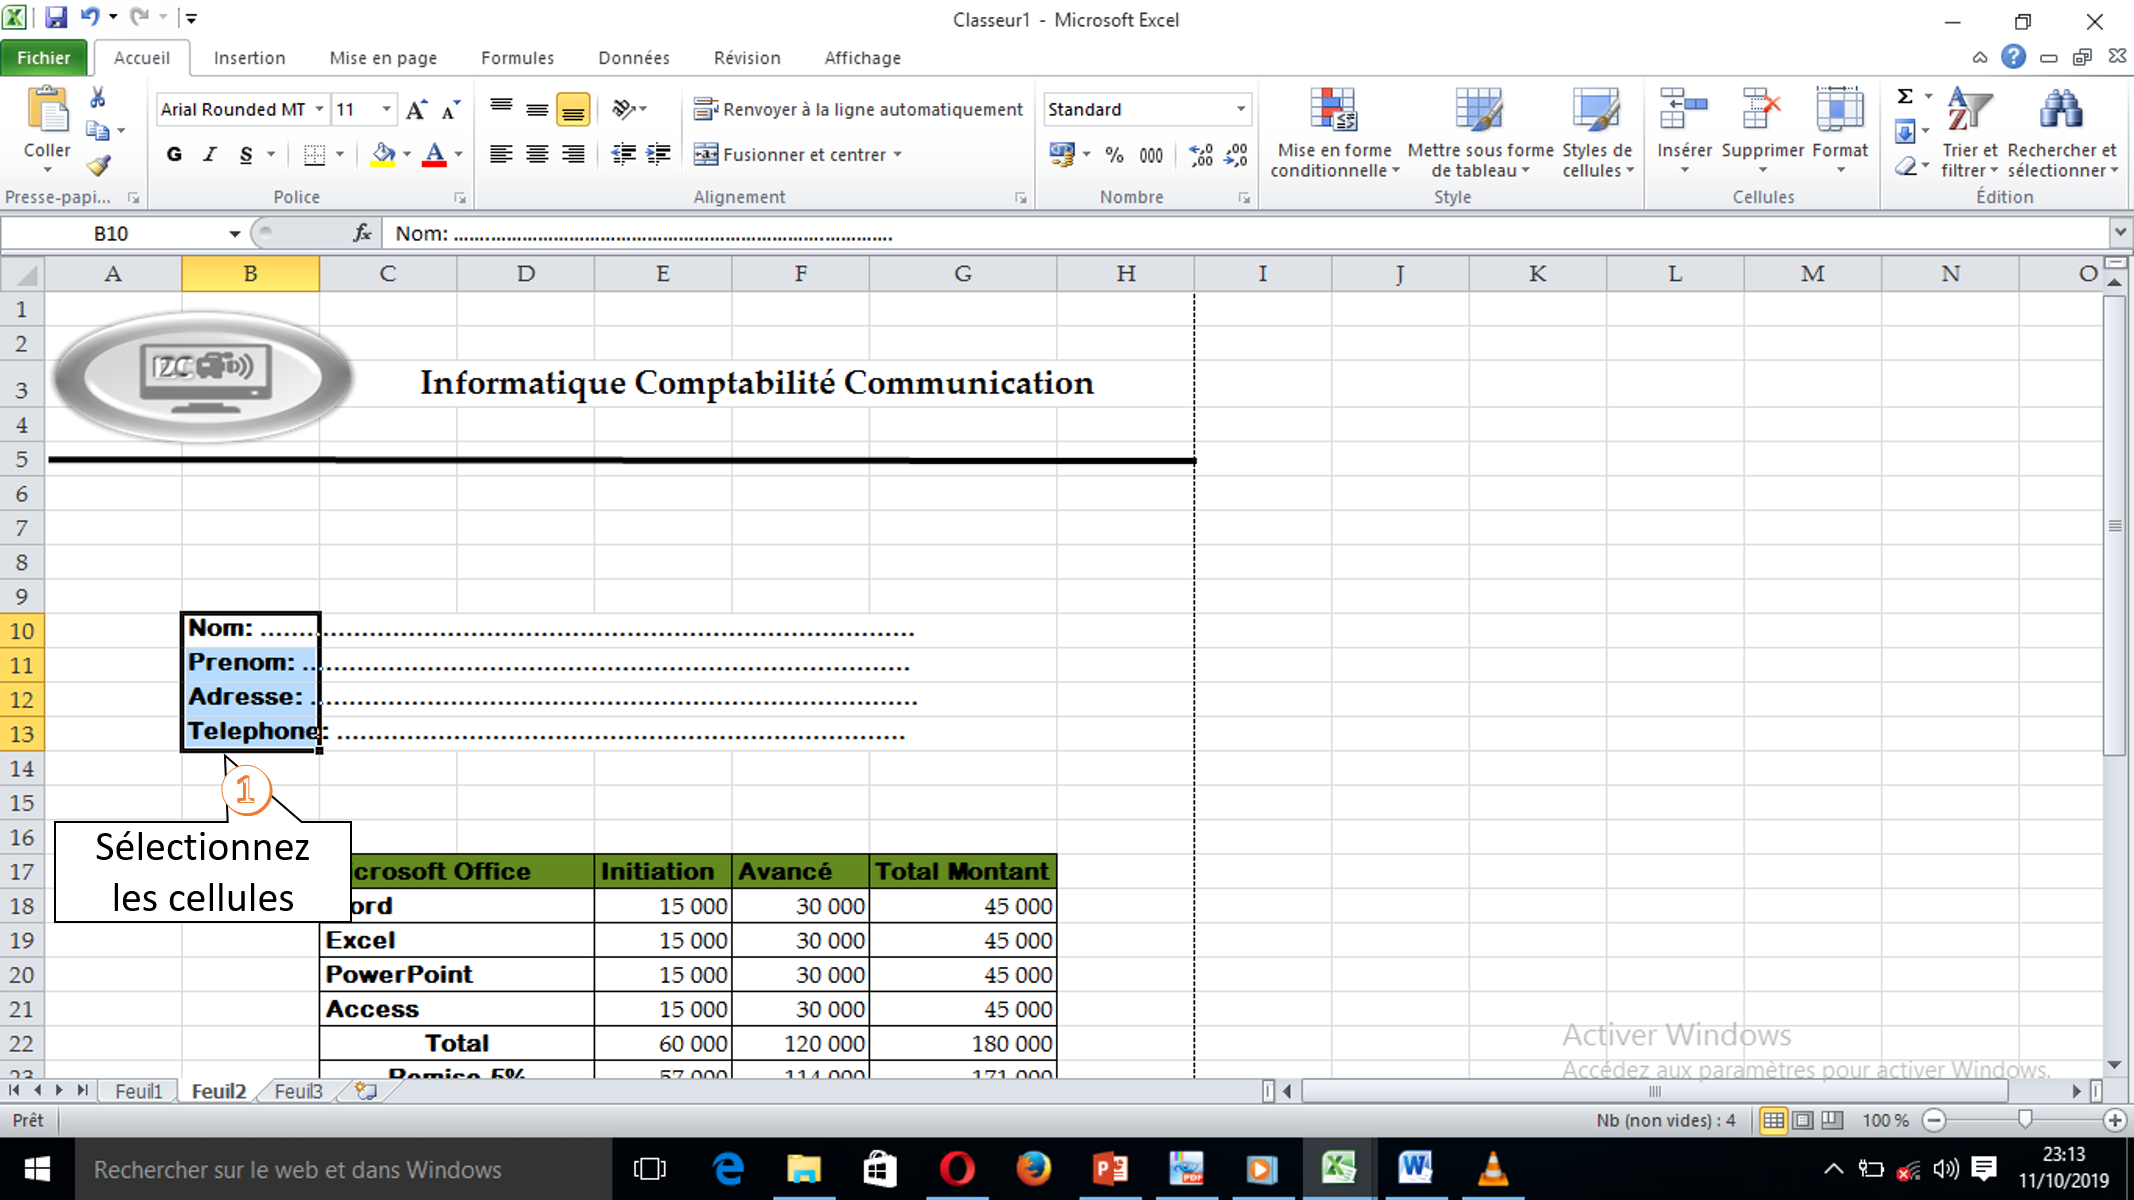
\includegraphics[ width=\linewidth,height=0.705\paperheight]{img/44}
\end{landscape}
\begin{landscape} 		
	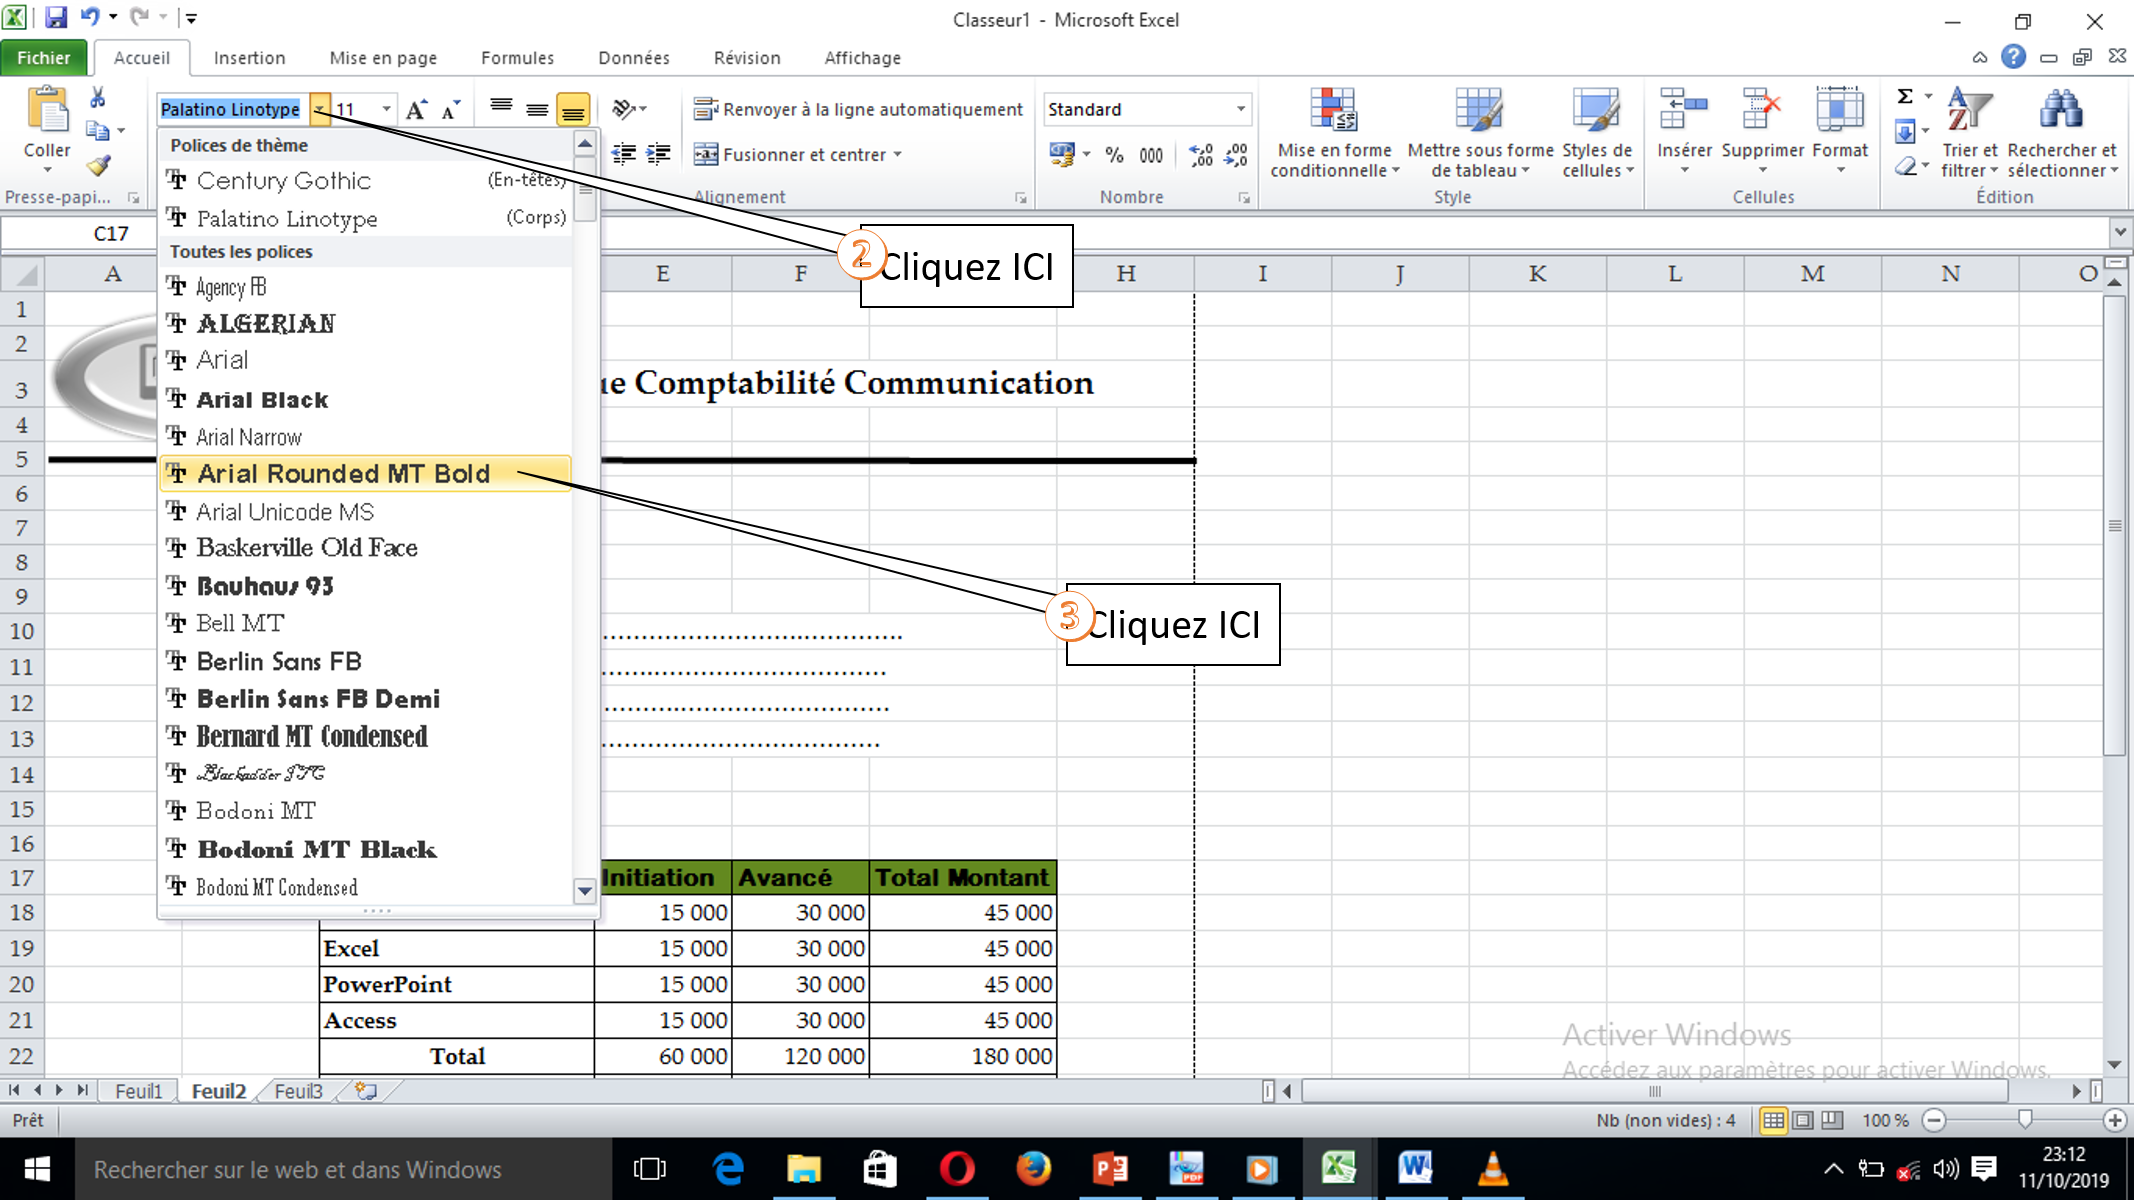
\includegraphics[ width=\linewidth,height=0.705\paperheight]{img/45}
\end{landscape}
\begin{landscape} 		
	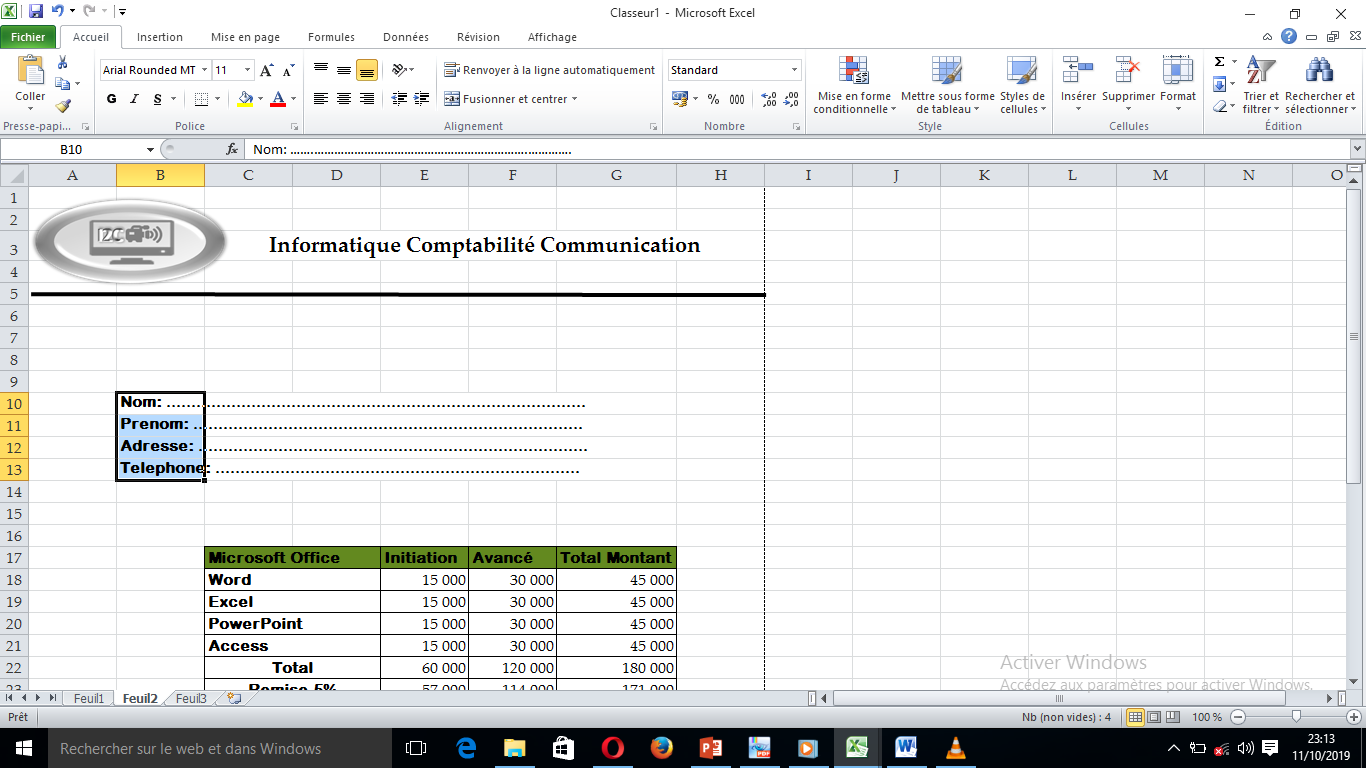
\includegraphics[ width=\linewidth,height=0.705\paperheight]{img/46}
\end{landscape}
\begin{landscape} 		
	\includegraphics[ width=\linewidth,height=0.705\paperheight]{img/47}
\end{landscape}
\begin{landscape} 		
	\includegraphics[ width=\linewidth,height=0.705\paperheight]{img/48}
\end{landscape}
\begin{landscape} 		
	\includegraphics[ width=\linewidth,height=0.705\paperheight]{img/49}
\end{landscape}
\begin{landscape} 		
	\includegraphics[ width=\linewidth,height=0.705\paperheight]{img/50}
\end{landscape}
\begin{landscape} 		
	\includegraphics[ width=\linewidth,height=0.705\paperheight]{img/51}
\end{landscape}
\begin{landscape} 		
	\includegraphics[ width=\linewidth,height=0.705\paperheight]{img/52}
\end{landscape}
\begin{landscape} 		
	\includegraphics[ width=\linewidth,height=0.705\paperheight]{img/53}
\end{landscape}

\part{Operations Arithmetiques}

\begin{landscape} 		
	\includegraphics[ width=\linewidth,height=0.705\paperheight]{img/54}
\end{landscape}
\begin{landscape} 		
	\includegraphics[ width=\linewidth,height=0.705\paperheight]{img/55}
\end{landscape}
\begin{landscape} 		
	\includegraphics[ width=\linewidth,height=0.705\paperheight]{img/56}
\end{landscape}
\begin{landscape} 		
	\includegraphics[ width=\linewidth,height=0.705\paperheight]{img/57}
\end{landscape}
\begin{landscape} 		
	\includegraphics[ width=\linewidth,height=0.705\paperheight]{img/58}
\end{landscape}
\begin{landscape} 		
	\includegraphics[ width=\linewidth,height=0.705\paperheight]{img/59}
\end{landscape}
\begin{landscape} 		
	\includegraphics[ width=\linewidth,height=0.705\paperheight]{img/60}
\end{landscape}
\begin{landscape} 		
	\includegraphics[ width=\linewidth,height=0.705\paperheight]{img/61}
\end{landscape}
\begin{landscape} 		
	\includegraphics[ width=\linewidth,height=0.705\paperheight]{img/62}
\end{landscape}
\begin{landscape} 		
	\includegraphics[ width=\linewidth,height=0.705\paperheight]{img/63}
\end{landscape}

\part{Prise en Page}
\begin{landscape} 		
	\includegraphics[ width=\linewidth,height=0.705\paperheight]{img/64}
\end{landscape}
\begin{landscape} 		
	\includegraphics[ width=\linewidth,height=0.705\paperheight]{img/65}
\end{landscape}
\begin{landscape} 		
	\includegraphics[ width=\linewidth,height=0.705\paperheight]{img/66}
\end{landscape}
\begin{landscape} 		
	\includegraphics[ width=\linewidth,height=0.705\paperheight]{img/67}
\end{landscape}
\begin{landscape} 		
	\includegraphics[ width=\linewidth,height=0.705\paperheight]{img/68}
\end{landscape}
\begin{landscape} 		
	\includegraphics[ width=\linewidth,height=0.705\paperheight]{img/69}
\end{landscape}

\part{Fonction Conditionelle}
\begin{landscape} 		
	\includegraphics[ width=\linewidth,height=0.705\paperheight]{img/70}
\end{landscape}
\begin{landscape} 		
	\includegraphics[ width=\linewidth,height=0.705\paperheight]{img/71}
\end{landscape}
\begin{landscape} 		
	\includegraphics[ width=\linewidth,height=0.705\paperheight]{img/72}
\end{landscape}
\begin{landscape} 		
	\includegraphics[ width=\linewidth,height=0.705\paperheight]{img/73}
\end{landscape}
\begin{landscape} 		
	\includegraphics[ width=\linewidth,height=0.705\paperheight]{img/74}
\end{landscape}
\begin{landscape} 		
	\includegraphics[ width=\linewidth,height=0.705\paperheight]{img/75}
\end{landscape}

\part{Mise en Forme Conditionnelle}
\begin{landscape} 		
	\includegraphics[ width=\linewidth,height=0.705\paperheight]{img/76}
\end{landscape}
\begin{landscape} 		
	\includegraphics[ width=\linewidth,height=0.705\paperheight]{img/77}
\end{landscape}
\begin{landscape} 		
	\includegraphics[ width=\linewidth,height=0.705\paperheight]{img/78}
\end{landscape}

\part{Impression}
\begin{landscape} 		
	\includegraphics[ width=\linewidth,height=0.705\paperheight]{img/79}
\end{landscape}
\begin{landscape} 		
	\includegraphics[ width=\linewidth,height=0.705\paperheight]{img/80}
\end{landscape}

\part{Graphiques}

\begin{landscape} 		
	\includegraphics[ width=\linewidth,height=0.705\paperheight]{img/81}
\end{landscape}
\begin{landscape} 		
	\includegraphics[ width=\linewidth,height=0.705\paperheight]{img/82}
\end{landscape}
\begin{landscape} 		
	\includegraphics[ width=\linewidth,height=0.705\paperheight]{img/83}
\end{landscape}
\begin{landscape} 		
	\includegraphics[ width=\linewidth,height=0.705\paperheight]{img/84}
\end{landscape}
\begin{landscape} 		
	\includegraphics[ width=\linewidth,height=0.705\paperheight]{img/85}
\end{landscape}
\begin{landscape} 		
	\includegraphics[ width=\linewidth,height=0.705\paperheight]{img/86}
\end{landscape}
	\newpage
	\clearpage
  
	\clearpage
	\nopagebreak
 	
 	
\end{document}
